\documentclass[a5paper,14pt]{report}
\usepackage{amsmath}
\usepackage{amssymb}
\usepackage[english, russian]{babel}
%\usepackage[cp1251]{inputenc}
\usepackage[T1,T2A]{fontenc} %added
\usepackage[utf8]{inputenc}
\usepackage[dvips]{graphicx}
\graphicspath{{images/}}
\usepackage{indentfirst}
\usepackage{multicol}
\usepackage{hhline}
\usepackage{multirow}
\usepackage{textcomp}
\usepackage{wrapfig}
\usepackage{color,colortbl}
\definecolor{Gray1}{gray}{0.7}
\definecolor{Gray2}{gray}{0.6}
\definecolor{Gray3}{gray}{0.5}
\definecolor{Gray4}{gray}{0.4}
\usepackage{geometry}
\geometry{left=1.5cm}
\geometry{right=1.5cm}
\geometry{top=1cm}
\geometry{bottom=2cm}
\newcommand*{\hm}[1]{#1\nobreak\discretionary{}{\hbox{$\mathsurround=0pt #1$}}{}}


\begin{document}

\begin{titlepage}
Балакшин П.В., Соснин В.В., Машина Е.А.  Информатика. – СПб: Университет ИТМО, 2018. – 122 с.
\\\\\textbf{TO REVIEW AND REWRITE!!!!} В пособии излагаются основные понятия, необходимые для более глубокого изучения компьютерной техники и систем в будущем. Рассматриваются основные принципы построения, функционирования и организации памяти ЭВМ. Предлагается изучить несколько пакетов, в том числе систему компьютерной верстки TeX, и некоторые варианты распознавания того, что данные были переданы с ошибкой.
\\\\\\\\Рекомендовано к печати Ученым советом факультета программной инженерии и компьютерной техники. 
\vspace{5 cm}
\begin{flushright}

\includegraphics[width=5cm]{ITMO_log}
\end{flushright}
Университет ИТМО – ведущий вуз России в области информационных и фотонных технологий, один из немногих российских вузов, получивших в 2009 году статус национального исследовательского университета. С 2013 года Университет ИТМО – участник программы повышения конкурентоспособности российских университетов среди ведущих мировых научно-образовательных центров, известной как проект «5 в 100». Цель Университета ИТМО – становление исследовательского университета мирового уровня, предпринимательского по типу, ориентированного на интернационализацию всех направлений деятельности. 
\begin{flushright}
\copyright Университет ИТМО, 2020
\\\copyright Балакшин П.В., Соснин В.В., 2020
\end{flushright}
\end{titlepage}

\tableofcontents
%DONE
\newpage
\textbf{О курсе\\}
\section{О курсе}

Цель данного методического пособия состоит в изучении общих принципов работы компьютера и получении навыков работы с рядом пакетов. Студентам предлагается рассмотреть для получения базовых знаний и умений по работе с компьютером такие темы как: 
\begin{itemize}

\item основы теории информации;
\item сжатие компьютерных данных;
\item помехоустойчивое кодирование;
\item архитектура ЭВМ;
\item организация компьютерных сетей;
\item работа с офисными пакетами;
\item программное обеспечение профессионального программиста.
\end{itemize}

Наряду с этими темами, авторы этого пособия предоставляют возможность более детально ознакомиться с рядом современных пакетов, в их числе такие широко известные продукты Microsoft, как Microsoft Office Word и Microsoft Excel, и система компьютерной верстки TeX, имеющая свой собственный язык разметки. Освоение указанных пакетов позволит студентам получить полезные навыки по подготовке презентаций, научно-технических отчетов о результатах выполненной работы, в оформлении результатов исследований в виде статей и докладов на научно-технических конференциях. Также авторы пособия продемонсрируют не-которые методики использования программных средств для решения практических задач.


\newpage
\textbf{Введение в информатику\\}
\section{Терминология информатики}

Начать изучение информатики невозможно, не разобравшись в точном значении термина «информатика». Однако, до сих пор в мировой научной общественности не сложилось четкого понимания этого термина. Рассмотрим одно из популярных определений:

\textbf{Информатика} – дисциплина, изучающая свойства и структуру информации, закономерности ее создания, преобразования, накопления, передачи и использования. За рубежом сложилась чуть более узкая трактовка термина информатика. Там под этим понимают пересечение сразу трех областей науки – это информационные технологии, теория информации и computer science. Всё обозначенное выше подходит под определение самого курса "Информатика".

Изучая некоторую науку важно представлять основные даты, вехи её развития:
\begin{itemize}
\item 1956(57) – появление термина «информатика» (\textit{нем.} Informatik, Штейнбух).
\item 1968 – первое упоминание в СССР (информология, Харкевич).
\item 197Х – информатика стала отдельной наукой.
\item 4 декабря – день российской информатики.
\end{itemize}

\newpage
\textbf{Основы теории информации\\}
\section{Терминология теории информации}

Рассмотрим некоторые терминологические тонкости. В обыденном языке, слова <<информация>> и <<данные>> считаются синонимами. Они, как правило, употребляются взаимозаменяемо. И так обстоит дело в информатике и в целом, в компьютерных науках.



Понятие \textit{"информация"} имеет различные трактовки в различных предметных областях. Например,\textit{информация} может пониматься как:
\begin{itemize}
\item сигналы для управления, приспособления рассматриваемой системы (в кибернетике);
\item мера хаоса в рассматриваемой системе (в физике);
\item вероятность выбора в рассматриваемой системе (в теории вероятностей);
\item мера разнообразия в рассматриваемой системе (в биологии) и др.
\end{itemize}
 Но мы остановимся на понятиях, близких к информатике.
\\
\\\textbf{Информация} - это некоторая упорядоченная последовательность сообщений, отражающих, передающих и увеличивающих наши знания.
\\
\\\textbf{Информация} - это сведения об окружающем мире (объекте, процессе, явлении, событии), которые являются объектом преобразования (включая хранение, передачу и т.д.) и используются для выработки поведения, для принятия решения, для управления или для обучения.
\\
\\\textbf{Информация} - это новые сведения, подлежащие передаче, хранению и обработке.s
\newpage 
Рассмотрим это фундаментальное понятие информатики на основе понятия \textit{"алфавит"} ("алфавитный", формальный подход). Дадим формальное определение \textit{алфавита}.
\\
\\\textbf{Алфавит} - конечное множество различных знаков (букв), символов, для которых определена операция \emph{конкатенации} (присоединения символа к символу или цепочке символов); с ее помощью по определенным правилам соединения символов и слов можно получать слова (цепочки знаков) и словосочетания (цепочки \textit{слов}) в этом \textit{алфавите} (над этим \textit{алфавитом}).
\\
\\\textbf{Знак (буква)} - любой элемент алфавита (элемент $x$ алфавита $X$, где $x \in X$). Понятие знака неразрывно связано с тем, что им обозначается ("со смыслом"), они вместе могут рассматриваться как пара элементов ($x$, $y$), где $x$ – сам знак, а $y$ – обозначаемое этим знаком.\\
\\\emph{\textbf{Пример 1:}}
\\Примеры \emph{алфавитов:} множество из десяти цифр, множество из знаков русского языка, точка и тире в азбуке Морзе и др. В \emph{алфавите} цифр знак 5 связан с понятием "быть в количестве пяти элементов".\\
\\\textbf{Слово} в алфавите (или над алфавитом) - конечная последовательность знаков (букв) алфавита.
\\
\\\textbf{Длина} |p| некоторого слова $p$ в алфавите (над алфавитом) - число составляющих его букв.
\\
\\\textbf{Словарь (словарный запас)} - множество различных слов в алфавите (над алфавитом).
\\В отличие от конечного \emph{алфавита}, словарный запас может быть и бесконечным.\\
\\\emph{Слова} над некоторым заданным \emph{алфавитом} и определяют так называемые \emph{сообщения}.\\
\\\emph{\textbf{Пример 2:}}
\\\emph{Слова} над \emph{алфавитом} кириллицы - "Информатика","инто", "ииии'', "и". 
\\\emph{Слова} над \emph{алфавитом} десятичных цифр и знаков арифметических операций – "1256", "23+78", "35–6+89", "4". 
\\\emph{Слова} над \emph{алфавитом} азбуки Морзе – ".", ". . –", "– – –".\\
\\В  \emph{алфавите} должен быть определен порядок следования \emph{букв} (порядок типа "предыдущий элемент – последующий элемент"), то есть любой \emph{алфавит} имеет упорядоченный вид $X = {x_1, x_2, …, x_n}$ .\\
\\Таким образом, \emph{алфавит} должен позволять решать задачу лексикографического (алфавитного) упорядочивания, или задачу расположения \emph{слов} над этим \emph{алфавитом}, в соответствии с порядком, определенным в \emph{алфавите} (то есть по символам \emph{алфавита}).

\section{Признаки классификации информации}

Рассмотрим две классификации информации. Первая из них - классификация по форме \emph{сообщений} - определенного вида сигналов, символов:
\begin{itemize}
  \item отношение к источнику или приемнику (входная, выходная и внутренняя);
  \item отношение к конечному результату (исходная, промежуточная и результирующая);
  \item актуальность;
  \item адекватность;
  \item доступность (открытая, закрытая);
  \item понятность;
  \item полнота (достаточная, недостаточная, избыточная);
  \item достоверность;
  \item массовость;
  \item изменчивость (постоянная, переменная, смешанная);
  \item объективность;
  \item точность;
  \item стадия использования (первичная, вторичная);
  \item ценность.
\end{itemize}

Вторая классификация - по форме преставления информации, способам ее кодирования и хранения:
\begin{itemize}
  \item графическая;
  \item звуковая;
  \item текстовая;
  \item числовая;
  \item видеоинформация.
\end{itemize}

\section{Измерение количества информации}
Любые сообщения измеряются в \emph{байтах, килобайтах, мегабайтах, гигабайтах, терабайтах, петабайтах} и \emph{эксабайтах}, а кодируются, например, в компьютере, с помощью \emph{алфавита} из нулей и единиц, записываются и реализуются в ЭВМ в \emph{битах}.

Приведем основные соотношения между единицами измерения \emph{сообщений}:
\begin{itemize}
\item 1 бит (\textbf{bi}nary digi\textbf{t} - двоичное число) = 0 или 1;
\item 1 байт = 8 бит;
\item 1 килобайт (1Кб) = $2^{13}$ бит;
\item 1 мегабайт (1Мб) = $2^{23}$ бит;
\item 1 гигабайт (1Гб) = $2^{33}$ бит;
\item 1 терабайт (1Тб) = $2^{43}$ бит;
\item 1 петабайт (1Пб) = $2^{53}$ бит;
\item 1 эксабайт (1Эб) = $2^{63}$ бит.
\end{itemize}

Теперь нам известно понятие информации, но необходимо еще конкретно знать сколько этой информации. Поэтому есть два важных определения:
\\
\\\textbf{Количество информации} - число, адекватно характеризующее разнообразие (структурированность, определённость,выбор состояний и т.д.) в оцениваемой системе. Количество информации часто оценивается в битах, причем такая оценка может выражаться и в долях бит (так как речь идет не об измерении или кодировании сообщений).
\\
\\\textbf{Мера информации} - численная оценка количества информации, которая обычно задана неотрицательной, определенной на множестве событий и являющейся аддитивной функцией (то есть, мера информации объединения событий (множеств) равна сумме мер каждого события). Заметим, что функция меры информации монотонна (при уменьшении или увеличении вероятности некоторого события количество иноформации в системе монотонно уменьшается или увеличивается). 
\\\textbf{Важно:} мера вероятности всегда находится в диапазоне от 0 до 1.
\par
Для измерения информации используются различные подходы и методы, например, с использованием меры информации по Р. Хартли и К. Шеннону.

\newpage
\subsection{Мера Хартли}

\begin{wrapfigure}{l}{2.7cm}
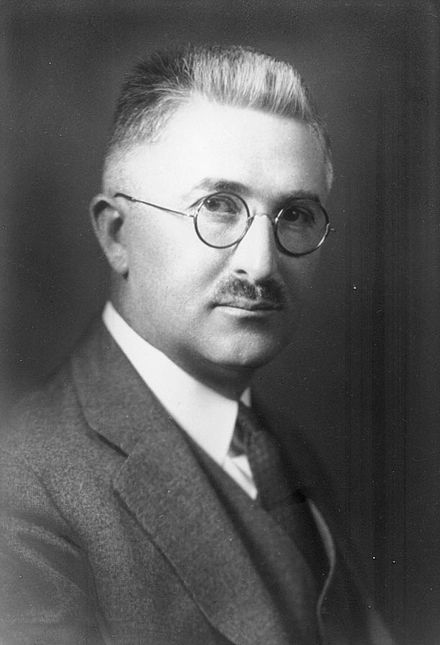
\includegraphics[width=2.7cm]{4_3_1}
\begin{center}
\footnotesize{Ральф Хартли}
\\\footnotesize{$1888 - 1970$}
\end{center}
\end{wrapfigure}

Пусть известны $N$ состояний системы $S$ ($N$  опытов с различными, равновозможными, последовательными состояниями системы). Если каждое состояние системы закодировать двоичными кодами, то минимальная длина $d$ полученного кода определяется из условия:

$$2^{d} \ge N \qquad \mbox{\emph{или}} \qquad  d \ge \log_{2}N$$
Значит, для однозначного описания системы требуется $\log_{2}N$ бит. В общем случае количество информации в системе $S$ равно:
$$H_{s} = \log_{k}N$$
Единицы измерения количества информации:
\begin{itemize}
  \item Бит ($k = 2$)
  \item Трит ($k = 3$)
  \item Дит (харт) ($k = 10$)
  \item Нит (нат) ($k = e$)
\end{itemize}
\begin{center}
\textbf{Примеры использования меры Хартли}
\end{center}
\emph{\textbf{Пример 1:}}
\\\emph{Задание:} мальчик загадывает число от 1 до 64. Какое количество вопросов типа "да-нет" понадобится, чтобы гарантированно угадать число?
\\\emph{Решение:}
\\$\bullet$ Первый вопрос: "Загаданное число меньше 32?". Ответ: "Да".
\\$\bullet$ Второй вопрос: "Загаданное число меньше 16?". Ответ: "Нет".
\\ \dots
\\$\bullet$ Шестой вопрос точно приведет к правильному ответу.
\\
\\Значит, в соответствии с мерой Хартли в загадке мальчика содержится $\log_{2}64 = 6$ бит информации ($N = 64$ так как возможно 64 вариантов загаданного числа).
\\Ответ: 6 бит.
\\
\\\emph{\textbf{Пример 2:}}
\\\emph{Задание:} мальчик держит за спиной шахматного ферзя и собирается поставить его на произвольную клетку пустой доски. Какое количество информации содержится в его действии?
\\\emph{Решение:} шахматная доска имеет размеры $8\times 8$ клеток. Ферзь может быть как белым, так и черным, поэтому количество равновероятных состояний будет равно $8\times 8 \times 2 = 128$. Получается, количество информации по мере Хартли равно $\log_{2}128 = 7$ бит.
\\Ответ: 7 бит.
\\Если во множестве $X = {x_1,x_2, ..., x_n}$ искать произвольный элемент, то для его нахождения (по Хартли) необходимо иметь не менее $\log_{a}n$ (единиц) информации. 
\\Уменьшение $Н$ говорит об уменьшении разнообразия состояний $N$ системы, увеличение $Н$ говорит об увеличении разнообразия состояний $N$ системы.
\\
\\Мера Хартли подходит лишь для идеальных, абстрактных систем, так как в реальных системах состояния системы неодинаково осуществимы (неравновероятны).

\subsection{Мера Шеннона }
\begin{wrapfigure}[12]{l}{2.5cm}
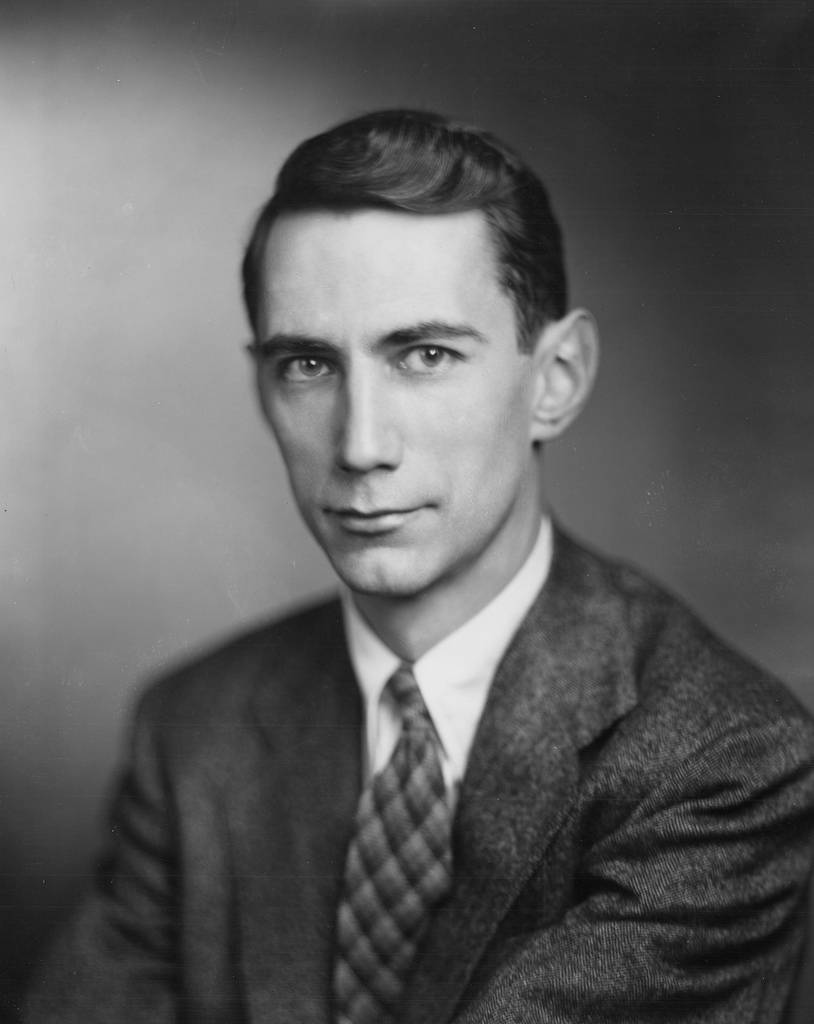
\includegraphics[width=2.5cm]{4_3_2}
\begin{center}
\footnotesize{Клод Шеннон}
\\\footnotesize{$1916 - 2001$}
\end{center}
\end{wrapfigure}

Если состояния системы не равновероятны, используют меру Шеннона. Мера Шеннона оценивает информацию отвлеченно от ее смысла:
$$I = - \sum^{N}_{i=1}p_{i}\times \log_{2}p_{i},$$ где:
\\$I$ - количество информации, выраженное в битах (в $\log_{k}p_{i}$ $k = 2$);
\\$N$ - число состояний системы;
\\$p_{i}$ - вероятность (относительная частота) перехода системы в $i$-е состояние (вероятность того, что система находится в состоянии $i$) \\Сумма всех $p_{i}$ должна быть равна единице.\\
\\Если все состояния рассматриваемой системы равновозможны, равновероятны, то есть $р_i = 1/n$ , то из \emph{формулы Шеннона} можно получить (как частный случай) \emph{формулу Хартли}:
$$I = \log_{2}n.$$
\\Обозначим величину:
$$f_i = -n\log_{2}p_i.$$
\newpage
Тогда из \emph{формулы К. Шеннона} следует, что количество информации I можно понимать как среднеарифметическое величин $f_i$ , то есть величину $f_i$ можно интерпретировать как \emph{информационное содержание символа алфавита} с индексом i и величиной $p_i$ вероятности появления этого символа в любом сообщении (слове), передающем информацию.\\
\\ В термодинамике известен так называемый коэффициент Больцмана $k = 1.38 * 10^{-16} (эрг.град)$ и выражение (\emph{формула Больцмана}) для энтропии или меры хаоса в термодинамической системе:
$$ S = -k \sum^{N}_{i=1}p_{i}\times \ln{p_{i}}$$
\\ Сравнивая выражения для I и S, можно заключить, что величину I можно понимать как энтропию из-за нехватки информации в системе (о системе).\\
\\Формулы энтропии и информации идентичны, но смысл разный. Энтропия априорная характеристика (до передачи), информация – апостериорная (после передачи).\\
\\Из этой формулы следуют важные выводы:
\begin{itemize}
\item увеличение меры Шеннона свидетельствует об уменьшении энтропии (увеличении порядка) системы;
\item уменьшение меры Шеннона свидетельствует об увеличении энтропии (увеличении беспорядка) системы.
\end{itemize}
Положительная сторона \emph{формулы Шеннона} – ее отвлеченность от смысла информации. Кроме того, в отличие от \emph{формулы Хартли}, она учитывает различность состояний, что делает ее пригодной для практических вычислений. Основная отрицательная сторона \emph{формулы Шеннона} – она не распознает различные состояния системы с одинаковой вероятностью.

\begin{center}
\textbf{Примеры использования меры Шеннона}
\end{center}
\emph{\textbf{Пример 1:}}
\\\emph{Задание:} девочка наугад вытаскивает из мешка мяч. Известно, что в мешке всего 8 мячей, из них: 4 красных, 2 синих, 1 зеленый и 1 белый. Какое количество информации содержится в этом событии?
\\\emph{Решение:}
\\$\bullet$ Вероятность вытащить красный мяч равна $^4/_8 = 0,5$
\\$\bullet$ Вероятность вытащить синий мяч равна $^2/_8 = 0,25$
\\$\bullet$ Вероятность вытащить зеленый мяч равна $^1/_8 = 0,125$
\\$\bullet$ Вероятность вытащить белый мяч равна $^1/_8 = 0,125$
\\Значит количество информации, выраженное в битах равно: $I = -(0,5\hm\times \log_{2}0,5\hm + 0,25\hm\times \log_{2}0,25 + 0,125\hm\times \log_{2}0,125\hm + 0,125\hm\times \log_{2}0,125) \hm = -(-0,5\times 1 - 0,25\times 2 - 0,125\times 3 - 0,125\times 3) = -(-0,5 - 0,5\hm - 0,375\hm - 0,375\hm) = 1,75$ бит.
\\Ответ: 1,75 бит

\section{Методы получения информации}
Методы получения информации можно разбить на три большие группы:
\begin{itemize}
\item \emph{Эмпирические};
\item \emph{Теоретические}; 
\item \emph{Эмпирико-теоретические}.
\end{itemize}
Кратко рассмотрим и охарактеризуем все три метода по отдельности. 
\subsection{Эмпирические методы}
\emph{Эмпирические методы или методы получения эмпирических данных.}
\begin{enumerate}
\item \emph{Наблюдение} -- сбор первичной информации об объекте, процессе, явлении.
\item \emph{Сравнение} -- обнаружение и соотнесение общего и различного.
\item \emph{Измерение} -- поиск с помощью измерительных приборов эмпирических фактов.
\item \emph{Эксперимент} -- преобразование, рассмотрение объекта, процесса, явления с целью выявления каких-то новых свойств.
\end{enumerate}
Кроме классических форм их реализации, в последнее время используются опрос, интервью, тестирование и другие.
\subsection{Теоретические методы}
\emph{Теоретические методы или методы построения различных теорий.}
\begin{enumerate}
\item \emph{Восхождение от абстрактного к конкретному} -- получение знаний о целом или о его частях на основе знаний об абстрактных проявлениях в сознании, в мышлении.
\item \emph{Идеализация} -- получение знаний о целом или его частях путем представления в мышлении целого или частей, не существующих в действительности.
\item \emph{Формализация} -- получение знаний о целом или его частях с помощью языков искусственного происхождения (формальное описание, представление).
\item \emph{Аксиоматизация} -- получение знаний о целом или его частях с помощью некоторых аксиом (не доказываемых в данной теории утверждений) и правил получения из них (и из ранее полученных утверждений) новых верных утверждений.
\item \emph{Виртуализация} -- получение знаний о целом или его частях с помощью искусственной среды, ситуации.
\end{enumerate}

\subsection{Эмпирико-теоретические методы}
\emph{Эмпирико-теоретические методы (смешанные) или методы построения теорий на основе полученных эмпирических данных об объекте, процессе, явлении.}
\begin{enumerate}
\item \emph{Абстрагирование} -- выделение наиболее важных для исследования свойств, сторон исследуемого объекта, процесса, явления и игнорирование несущественных и второстепенных.
\item \emph{Анализ} -- разъединение целого на части с целью выявления их связей.
\item \emph{Декомпозиция} -- разъединение целого на части с сохранением их связей с окружением.
\item \emph{Синтез} -- соединение частей в целое с целью выявления их взаимосвязей.
\item \emph{Композиция} -- соединение частей целого с сохранением их взаимосвязей с окружением.
\item \emph{Индукция} -- получение знания о целом по знаниям о частях.
\item \emph{Дедукция} -- получение знания о частях по знаниям о целом.
\item \emph{Эвристики, использование эвристических процедур} -- получение знания о целом по знаниям о частях и по наблюдениям, опыту, интуиции, предвидению.
\item \emph{Моделирование (простое моделирование)}, использование приборов -- получение знания о целом или о его частях с помощью модели или приборов.
\item \emph{Исторический метод} -- поиск знаний с использованием предыстории, реально существовавшей или же мыслимой.
\item \emph{Логический метод } -- поиск знаний путем воспроизведения частей, связей или элементов в мышлении.
\item \emph{Макетирование} -- получение информации по макету, представлению частей в упрощенном, но целостном виде.
\item \emph{Актуализация} -- получение информации с помощью перевода целого или его частей (а следовательно, и целого) из статического состояния в динамическое состояние.
\item \emph{Визуализация} -- получение информации с помощью наглядного или визуального представления состояний объекта, процесса, явления.
\end{enumerate}
Кроме указанных классических форм реализации теоретико-эмпирических методов часто используются и мониторинг (система наблюдений и анализа состояний), деловые игры и ситуации, экспертные оценки (экспертное оценивание), имитация (подражание) и другие формы.\\
\\\emph{\textbf{Пример :}}
\\Для построения модели планирования и управления производством в рамках страны, региона или крупной отрасли нужно решить следующие проблемы:
\begin{enumerate}
\item определить структурные связи, уровни управления и принятия решений, ресурсы; при этом чаще используются методы наблюдения, сравнения, измерения, эксперимента, анализа и синтеза, дедукции и индукции, эвристический, исторический и логический методы, макетирование и др.;
\item определить гипотезы, цели, возможные проблемы планирования; наиболее используемые методы – наблюдение, сравнение, эксперимент, абстрагирование, анализ, синтез, дедукция, индукция, эвристический, исторический, логический и др.;
\item конструирование эмпирических моделей; наиболее используемые методы – абстрагирование, анализ, синтез, индукция, дедукция, формализация, идеализация и др.;
\item поиск решения проблемы планирования и просчет различных вариантов, директив планирования, поиск оптимального решения; используемые чаще методы – измерение, сравнение, эксперимент, анализ, синтез, индукция, дедукция, актуализация, макетирование, визуализация, виртуализация и др.
\end{enumerate}

\chapter{Единицы измерения объема данных}
В области цифровой и вычислительной техники двоичная система счисления (основанная на степени двойки) получила широкое распространение. В следствие этого стали употреблять двоичные приставки:
\item $1 kB = 2^{10} B$ - $1$ килобайт равен $2^{10}$ байт;
\item $1 MB = 2^{20} B$ - $1$ мегабайт равен $2^{20}$ байт.
\\Однако, такая система противоречит СИ, которая использует десятичные приставки (основанные на степени десяти):
\item $1 k = 10^{3}$, $1 M = 10^{6}$.
\\Поначалу это противоречие не было существенной проблемой. Число $2^{10} = 1024$ достаточно близко к тысяче и при объемах памяти, измерявшихся килобайтами, ошибка была всего в 2,4\%. Но по мере развития технологий, разница между "двоичным" и "десятичным" гигабайтом была в 7\%.

\\Тогда IEEE, Институт инженеров электротехники и электроники (англ. Institute of Electrical and Electronics Engineers), утвердил стандарт IEEE 1541-2002. Также существуют стандарты  ISO/IEC 80000-13:2008, принятый международной организацией по стандартизации и ГОСТ IEC 60027-2-2015, принятый междунагодной электротехнической комиссией.
\\
\begin{center}
Рекомендации стандарта IEEE 1541-2002
\end{center}
\begin{itemize}
\item Бит (bit) (символ 'b') - двоичный знак;
\item Байт (byte) (символ 'B') - равен 8 битам ($1B = 8b$);
\item Киби (kibi) (символ 'Ki') - $2^{10} = 1024$;
\item Меби (mebi) (символ 'Mi') - $2^{20} = 1048576$;
\item Гиби (gibi) (символ 'Gi') - $2^{30} = 1073741824$;
\item Теби (tebi) (символ 'Ti') - $2^{40} = 1099511627776$.
\end{itemize}

Сегодня в кибибайтах, мебибайтах и т.д. измеряется память - оперативная память, жесткие диски, flash-накопители. Однако, скорость передачи данных измеряется в килобайтах и мегабайтах в секунду (например, 512 kbps (kilobits per second) - 512 килобит в секунду).
Операционные системы считают по-разному. *nix системы (unix, linux) используют "двоичные" приставки, в то время как Windows использует приставки СИ. 

\chapter{Системы счисления}
В истории разные народы использовали системы счисления с разными основаниями. Каждый народ руководствовался своими доводами в пользу того или иного числа в основании. Например, африканские племена использовали 5-ричную систему счисления, потому что на руке 5 пальцев. Тибетцы и нигерийцы использовали 12-ричную, это количество фаланг на четырех пальцах. Привычная нам система счисления с основанием равным 10 появилась в Европе в 16, а в России в 17 веке.
\begin{figure} [h!]
\center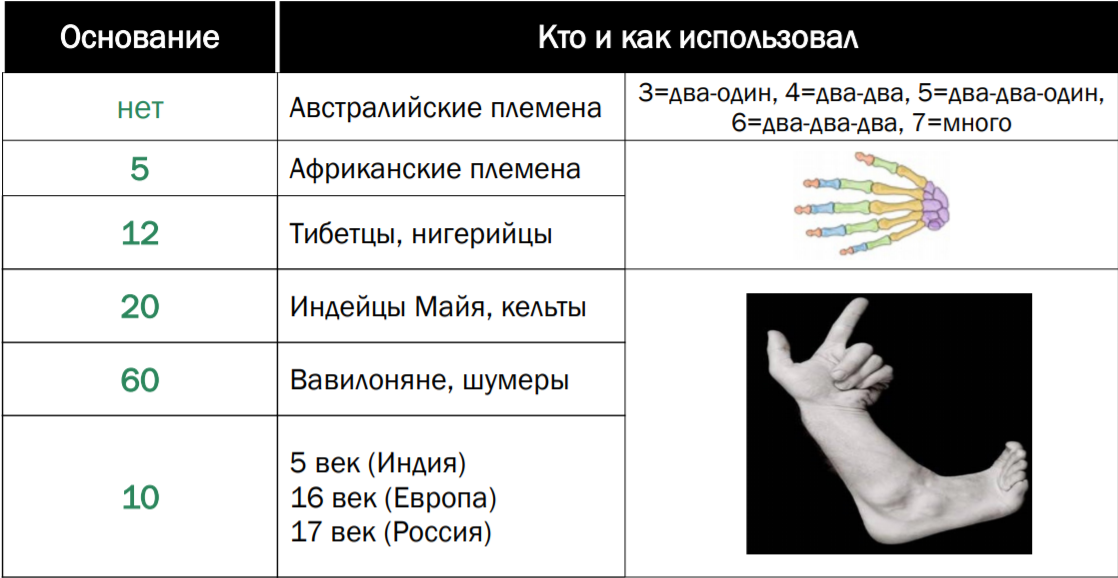
\includegraphics[width=\textwidth]{images/2_1.png}
\caption{Различные системы счисления}
\end{figure}

\section{Позиционная система счисления}

Рассмотрим формулу записи числа в позиционной системе счисления:
\\$X_{(q)} = x_{n-1}\times q^{n-1} + x_{n-2}\times q^{n-2} + ... + x_{1}\times q^{1} + x_{0}\times q^{0} + x_{-1}\hm\times q^{-1}\hm + x_{-2}\hm\times q^{-2}\hm + ... + x_{-m}\times q^{-m}.$
\\Или
\\$$X_{(q)} = \sum_{i=-m}^{n-1} x_{i}\times q^{i},$$
\\где:
\\$X_{(q)}$ - запись числа в системе счисления с основанием $q$;
\\$x_{i}$ - натуральные числа меньше $q$, то есть цифры;
\\$n$ - число разрядов целой части;
\\$m$ - число разрядов дробной части;
\\$q$ - показатель системы счисления.
\\
\\Само число $X_{(q)}$ имеет следующий вид:
\\$$X_{(q)} = x_{n-1}x_{n-2}...x_{1}x_{0}x_{-1}...x_{1-m}x_{-m}.$$
\\Рассмотрим данную формулу на примере:
\\$123,45_{10} = 1\times 10^{2} + 2\times 10^{1} + 3\times 10^{0} + 4\times 10^{-1} + 5\times 10^{-2}$
\\Мы разложили число $123,45$ по этой формуле. В данном случае $q$ = 10, $n$ = 3, $m$ = 2, $X_{(q)} = 123,45$, а $x_{3-1} = 1$ ($x_{2} = 1$), $x_{1} = 2$ и так далее.
\\В позиционной системе счисления важную роль имеет порядок цифр, то есть значение каждого числового знака (цифры) в записи числа зависит от его позиции (разряда).

\section{Перевод чисел из одной системы счисления в другую}

Существуют три способа перевода из одной системы счисления в другую:
\begin{enumerate}
\item Из десятичной системы счисления в систему счисления с основанием $N$.
\item Из системы счисления с основанием $N$ в десятичную систему счисления.
\item Из системы счисления с основанием $N$ в систему счисления с основанием $N^{k}$ и обратно, при условии $k \in \mathbb{N}$.
\end{enumerate}

\subsection{Перевод числа из десятичной системы счисления в систему счисления с основанием $N$}
Чтобы перевести дробное число в систему счисления с основанием $N$ необходимо разделить его на две части: целую и дробную, и каждую часть переводить отдельно.
\subsubsection{Преобразования целой части числа}
Для перевода целой части числа из десятичной системы счисления в другую необходимо:
\begin{enumerate}
\item Разделить целую часть десятичного числа на основание новой системы счисления.
\item Записать остаток деления.
\item Разделить получившийся результат деления (п.1) на основание новой системы счисления (при необходимости).
\item Записать остаток деления.
\end{enumerate}
Повторять, пока целая часть десятичного числа не будет равна 0.
\\Получившиеся в ходе деления остатки и есть цифры искомого числа в новой системе счисления. Записать остатки в обратном порядке (начиная с последнего полученного). Стоит заметить, что в данном способе очень удобно применять деление столбиком.
\\
\\\emph{\textbf{Пример 1:}}
\\\emph{Задание:} перевести число $45_{10}$ в троичную систему счисления.
\\\emph{Решение:} последовательно разделим $45_{10}$ на $3$, записывая остатки:
\begin{figure}[h]
\centering
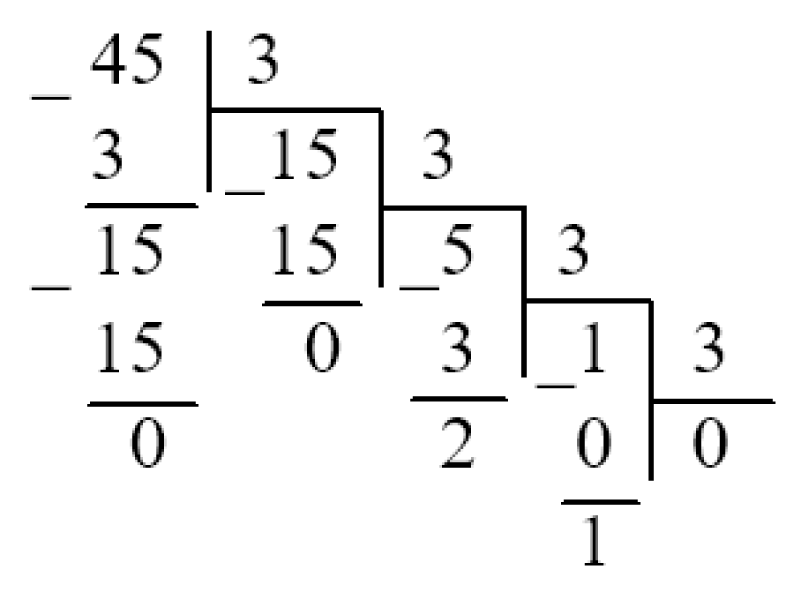
\includegraphics[width=4cm]{1_2_1(1)}
\caption{Последовательное деление $45_{10}$ на $3$.}
\end{figure}
\\Полученные остатки: 0, 0, 2, 1. Записываем их в обратном порядке.
\\Ответ:$45_{10} = 1200_{3}$

\subsubsection{Преобразования дробной части числа}
Для перевода дробной части числа из десятичной системы счисления в другую необходимо:
\begin{enumerate}
\item Умножить дробную часть десятичного числа на основание новой системы счисления.
\item Отделить и записать целую часть.
\item Умножить дробную часть результата умножения (п.1) на основание новой системы счисления (при необходимости).
\item Отделить и записать целую часть.
\end{enumerate}
Повторять, пока дробная часть десятичного числа не будет равна 0.
\\Получившиеся в ходе умножения целые части и есть цифры искомого числа в новой системе счисления. Записать целые части в прямом порядке (начиная с первого полученного). Первая записанная целая часть (0) идет в целую часть нового числа, а в дробную записываются полученные целые части, начиная со второй. Стоит заметить, что в данном способе очень удобно применять умножение столбиком.
\\
\\\emph{\textbf{Пример 2:}}
\\\emph{Задание:} перевести число $0,625_{10}$ в четверичную систему счисления.
\\\emph{Решение:} умножим дробную часть $0,625_{10}$ на $4$, записывая целые части, пока не получим в дробной части 0:
\begin{figure}[h]
\centering
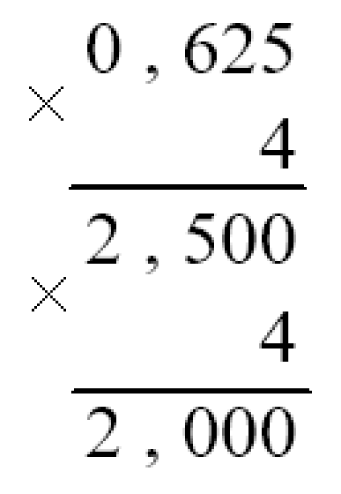
\includegraphics[width=1.7cm]{1_2_1(2)}
\caption{Умножение $0,625_{10}$ на $4$ до получения 0 в дробной части.}
\end{figure}
\\\emph{Пояснение: сначала умножаем 0,625 на 4, получаем 2,5. 2 записываем в целые части, а далее используем дробную часть -- 0,5. Умножаем 0,5 на 4, получаем 2, записываем в целые части. Так как дробная часть равна 0, то перевод окончен.}
\\Полученные целые части: 0, 2, 2. Первая полученная целая часть (0) идет в целую часть нового числа. Остальные (2, 2) в дробную часть.
\\Ответ: $0,625_{10} = 0,22_{4}$.
\\
\\\emph{\textbf{Пример 3:}}
\\\emph{Задание:} перевести число $43,52_{10}$ в пятеричную систему счисления.
\\\emph{Решение:} разделим $43,52_{10}$ на две части: целую ($43_{10}$) и дробную ($0,52_{10}$). Переведем целую и дробную части по отдельности:
\begin{figure}[h]
\centering
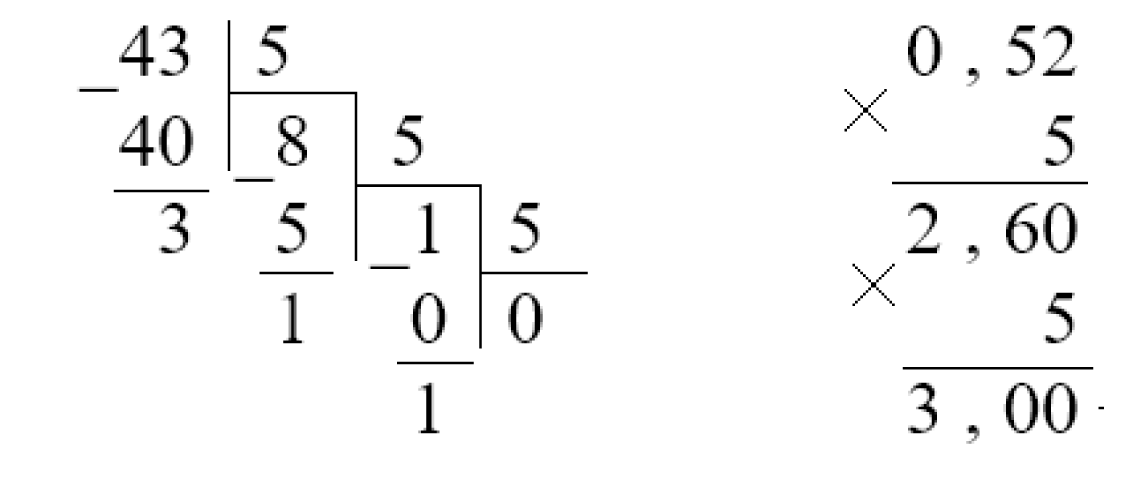
\includegraphics[width=6cm]{1_2_1(3)}
\caption{Перевод целой и дробной частей.}
\end{figure}
\\Полученные остатки (3, 1, 1) запишем в обратном порядке: $43_{10} = 113_{5}$
\\Полученные целые части (0, 2, 3) запишем в прямом порядке: $0,52_{10} = 0,23_{5}$
\\Объеденим полученные части
\\Ответ: $43,52_{10} = 113,23_{5}$.

\subsection{Перевод числа из системы счисления с основанием $N$ в десятичную систему счисления}
Формула перевода числа из системы счисления с основанием $N$ в десятичную систему счисления это практически формула записи числа в позиционной системе счисления.
$$X_{(10)} = \sum_{i=-m}^{n-1} x_{i}\times q^{i},$$
\\где:
\\$X_{(10)}$ - искомое число в десятичной системе счисления
\\$x_{i}$ - натуральные числа меньше $q$, то есть цифры
\\$n$ - число разрядов целой части
\\$m$ - число разрядов дробной части
\\$q$ - показатель системы счисления
\\
\\\emph{\textbf{Пример 1:}}
\\\emph{Задание:} перевести число $1101,111_{2}$ в десятичную систему счисления.
\\\emph{Решение:} $1101,111_{2} = 1\times 2^{3} + 1\times 2^{2} + 0\times 2^{1} + 1\times 2^{0} + 1\times 2^{-1} + 1\hm\times 2^{-2}\hm + 1\hm\times 2^{-3}\hm = 1\times 8 + 1\times 4 + 0\times 2 + 1\times 1 + 1\times 0,5 + 1\times 0,25 + 1\times 0,125\hm = 8 + 4 + 1 + 0,5 + 0,25 + 0,125 = 13,875_{10} $
\\Ответ: $1101,111_{2} = 13,875_{10}.$

\subsection{Перевод числа из системы счисления с основанием $N$ в систему счисления с основанием $N^{k}$ и обратно, при условии $k \in \mathbb{N}$}

Если основание системы счисления первого числа является степенью основания системы счисления второго числа ($N = N^{k}$), при условии $k \in \mathbb{N}$, то можно использовать следующий алгоритм.
\begin{center}
\center{\textbf{Преобразование $N \to N^{k}$}}
\end{center}

\begin{enumerate}
\item Дополнить число (записанное в системе счисления $N$) незначащими нулями так, чтобы количество цифр было кратно $k$ (если число дробное, то дополнить так, чтобы и в целой и в дробной частях количество цифр было кратно $k$).
\item Разбить это число на группы по $k$ цифр, начиная от нуля (если число дробное, то целую часть разбивать, начиная от запятой в левую сторону, а дробную часть, начиная от запятой в правую сторону).
\item Заменить каждую такую группу эквивалентным числом, записанным в системе $N^{k}$.
\end{enumerate}

\begin{center}
\center{\textbf{Преобразование $N^{k} \to N$}}
\end{center}

\begin{enumerate}
\item Заменить каждую цифру числа, записанного в системе счисления $N^{k}$, эквивалентным набором из $k$ цифр системы счисления $N$.
\end{enumerate}

Рассмотрим данный метод на системах счисления с основанием $N = 2^{k}$. Для этого воспользуемся таблицей.
%TODO:таблица поехала, поправить. она должна быть перед ПРИМЕР 1
\begin{table}[h!]
\caption{Основания вида $2^{k}$}
\centering
\begin{tabular}{|c|c|c|c|c|}
\hline
10--ая & 2--ая & 4--ая & 8--ая & 16--ая
\\\hline
0 & 0000 & 000 & 00 & 0
\\ 1 & 0001& 001 & 01 & 1
\\ 2 & 0010 & 002 & 02 & 2
\\ 3 & 0011 &003 & 03 & 3
\\ 4 & 0100 & 010 & 04 & 4
\\ 5 & 0101 & 011 & 05 & 5
\\ 6 & 0110 & 012 & 06 & 6
\\ 7 & 0111 & 013 & 07 & 7
\\ 8 & 1000 & 020 & 10 & 8
\\ 9 & 1001 & 021 & 11 & 9
\\ 10 & 1010 & 022 & 12 & A
\\ 11 & 1011 & 023 & 13 & B
\\ 12 & 1100 & 030 & 14 & C
\\ 13 & 1101 & 031 & 15 & D
\\ 14 & 1110 & 032 & 16 & E
\\ 15 & 1111 &300 & 17 & F
\\\hline
\end{tabular}
\end{table}

\emph{\textbf{Пример 1:}}
\\\emph{Задание:} пользуясь таблицей перевести число $1542,43_{8}$ в двоичную систему счисления
\\\emph{Решение:} по таблице находим чему равны цифры исходного числа в двоичной системе. $1_{8} = 001_{2}$, $5_{8} = 101_{2}$ (незначащие нули убираем, так как необходимо, чтобы количество цифр в эквивалентном наборе было равно степени $k$ из выражения $N = N^{k}$, где $N^{k}$ - исходная система счисления. В данном случае $k = 3$) и так далее.
\\Заменяем каждую цифру числа эквивалентным набором.
\\Ответ: $1542,43_{8} = 001101100010,100011_{2}$
\\

\emph{\textbf{Пример 2:}}
\\\emph{Задание:} пользуясь таблицей перевести число $11010,11_{2}$ в шестнадцатиричную систему счисления
\\\emph{Решение:} первым делом, добавим незначащие нули так, чтобы количество цифр было кратно $k$ (в данном случае $k = 4$). Так как число дробное, не забываем добавлять нули и в конце числа. \\Получим $00011010,1100_{2}$.
\\Теперь необходимо разбить число на группы по $k$ цифр (начинаем от запятой). Результат: $0001\ 1010\ ,\ 1100\ _{2}$.
\\Пользуясь таблицей, заменяем группы цифр эквивалентными числами, записанным в шестнадцатиричной системе счисления.
\\Ответ: $11010,11_{2} = 1A,C_{16}$.


\section{Оптимальная система счисления}
Давайте представим, что Вы по несчастливой (или счастливой) случайности попали на необитаемый остров. Обеспокоенный количеством дней, которые Вам суждено провести на острове в ожидании спасателей, Вы решаете вести счет дней с помощью камней. Но вот незадача - камней на острове нашлось всего 60 штук (небогатый на камни остров оказался). И для того, чтобы вести учет дней как можно продуктивнее (учесть как можно больше дней) необходимо выбрать систему счисления, плотность записи числа которой максимальна при данных обстоятельствах.
\\Существует зависимость плотности записи информации от основания системы счисления. Если взять $N$ камней, а за основание принять число $X$, то получится $^N/_X$ разрядов, которыми можно закодировать $X^{^N/_X}$ чисел.
\\То есть с помощью 60 камней мы можем закодировать: $2^{30}$, $3^{20}$, $4^{15}$, $5^{12}$, $6^{10}$, $10^{6}$, $12^{2}$, $15^{4}$, $20^{3}$, $30^{2}$ или $60^1$ чисел. Все зависит от того, какую систему счисления мы выберем. Возведя все числа в степени, мы увидим, что самое большое из них это $3^{20} = 3486784401$.
\\Удельная натуральнологарифмическая плотность записи числа зависит от основания системы счисления $х$ и выражается функцией $y = \frac{\ln{x}}{x}$. Эта функция имеет максимум при $x = e = 2,718281828...$.
\begin{figure}[h]
\centering
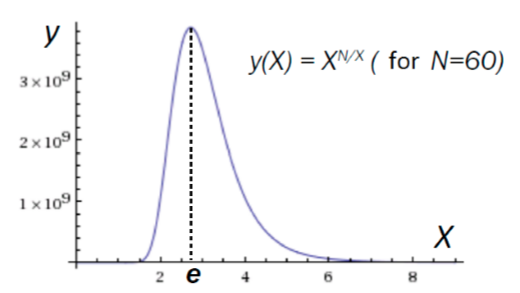
\includegraphics[width=6cm]{1_2_3(1)}
\end{figure}
\\Таким образом, самая оптимальная система счисления имеет основание равное $e = 2,718281828...$, то есть нецелочисленное. Она обладает наибольшей плотностью записи информации.
\\Возвращаясь к нашему пребыванию на острове, мы не можем взять дробное основание для системы счисления. Поэтому мы берем самое близкое целое к $e$ - это $3$.

\section{Округление чисел}

Как происходит округление чисел в десятичной системе счисления? Каждый учил в школе правила округления: 1, 2, 3, 4 округляется в меньшую сторону, а 5, 6, 7, 8 и 9 - в большую.
Рассмотрим два примера:
\\
\\
\begin{minipage}[c]{6cm}
\begin{center}
\begin{tabular}{|c|c|c|}
\hline  & Число & Округление
\\\hhline{~--} & 5,9 & 6,0
\\ & 4,1 & 4,0
\\ & 5,0 & 5,0
\\ & 6,6 & 7,0
\\ & 2,4 & 2,0
\\\hline Cумма & 24,0 & 24,0
\\\hline
\end{tabular}
\emph{Пример 1}
\newline
\end{center}
\end{minipage}
\begin{minipage}[c]{6cm}
\begin{center}
\begin{tabular}{|c|c|c|}
\hline & Число & Округление
\\\hhline{~--}  & 5,5 & 6,0
\\ & 3,5 & 4,0
\\ & 2,5 & 3,0
\\ & 8,5 & 9,0
\\ & 1,5 & 2,0
\\\hline Cумма & 21,5 & 24,0
\\\hline
\end{tabular}
\emph{Пример 2}
\newline
\end{center}
\end{minipage}


В примере 1 мы видим, что сумма до и после округления одинакова. Так случилось, потому что мы округляли то в большую сторону, то в меньшую, и в итоге количество округлений в большую сторону равно количеству округлений в меньшую. Округление нам не помешало получить красивую сумму.
\\А теперь посмотрим на специально подобранный пример 2. Разница сумм довольно большая. Так получилось, потому что мы округляли всегда только в большую сторону, хотя мы округляли по правилам.
\\Если проделать такой эксперимент с большим количеством чисел (тысяча, две тысячи или даже больше), то ошибка будет небольшая, но она будет.
\\Работая с числами, у которых показатель системы счисления четный, мы натыкаемся на следующую проблему: у нас нечетное количество чисел для округления. Разберем на примере десятичной системы счисления. В ней всего 10 цифр - 0, 1, 2, 3, 4, 5, 6, 7, 8, 9. Числа $X.0$ мы не округляем. Остается 9 чисел: $X.1$, $X.2$, $X.3$, $X.4$ округляем в меньшую сторону (всего 4 числа), а $X.5$, $X.6$, $X.7$, $X.8$, $X.9$ - в большую (всего 5 чисел). $X.5$ - середина между $X+1$ и $X$, однако мы округляем в пользу $X+1$, то есть в большую. Таким образом, при работе с большим количеством чисел, мы всегда будем округлять в большую сторону чаще, чем в меньшую. Отсюда и ошибка в итоговой сумме.
\\Чтобы этого избежать, некоторые программы при автоматическом округлении большого количества чисел округляют $X.5$ по очереди то в большую сторону, то в меньшую.
\\В системах счисления с нечетным основанием такой ошибки нет. Возьмем, к примеру, пятиричную систему счисления. Она содержит цифры 0, 1, 2, 3, 4. Числа $X.0$ мы не округляем, остается 4 числа: $X.1$, $X.2$ округляем в меньшую сторону (всего 2 числа), а $X.3$, $X.4$ - в большую (всего 2 числа). Таким образом, количество чисел, округленных в меньшую сторону, равно количеству чисел, округленных в большую.

\section{Нетрадиционные системы счисления}
\subsection{Факториальная система счисления}
Любое натуральное число можно представить в виде $$ X = \sum^{n}_{k = 1} d_{k}\times k! \qquad \mbox{,где  } 0 \leqslant d_{k} \leqslant k $$
\\В основании факториальной системы счисления используется факториал.
\\Запись числа в факториальной системе счисления будет иметь вид $$X_{\mbox{ф}} = d_{n}d_{n-1}...d_{1} $$

\subsubsection{Перевод из факториальной системы счисления в десятичную}
Алгоритм перевода из факториальной системы счисления в десятичную очень похож на алгоритм перевода из системы счисления с основанием $N$ в десятичную (раздел 2.2.1).
$$ X_{10} = d_{n}\times n! + d_{n-1}\times (n-1)! + d_{n-2}\hm\times (n-2)!\hm + ...\hm + d_{2}\times 2! + d_{1}\times 1!$$
Где:
\\$X_{10}$ - искомое число в десятичной системе счисления
\\$d_{i}$ - натуральные числа меньше или равные $i$
\\$n$ - количество разрядов исходного числа
\\
\emph{\textbf{Пример 1:}}
\\\emph{Задание:} перевести число $221_{\mbox{ф}}$ в десятичную систему счисления
\\\emph{Решение:} $221_{\mbox{ф}} = 2\times 3! + 2\times 2! + 1\times 1! = 2\times 6 + 2\times 2 + 1\times 1 = 12 + 4 + 1 = 17_{10}$
\\Ответ:  $221_{\mbox{ф}} = 17_{10}$
\subsubsection{Перевод из десятичной системы счисления в факториальную}
Для перевода воспользуемся все той же формулой:
$$ X_{10} = d_{n}\times n! + d_{n-1}\times (n-1)! + d_{n-2}\hm\times (n-2)!\hm + ...\hm + d_{2}\times 2! + d_{1}\times 1!$$
Стоит обратить внимание, что $0 \leqslant d_{1}\leqslant 1$; $0 \leqslant d_{2}\leqslant 2$ и так далее.
\begin{enumerate}
\item Находим факториал $k!$, значение которого больше $X_{10}$, но ближе всего к нему. Тогда $n = k - 1$, где $n$ - количество разрядов искомого числа в факториальной системе.
\item Записываем $$ X_{10} = d_{n}\times n! + d_{n-1}\times (n-1)! + d_{n-2}\hm\times (n-2)!\hm + ...\hm + d_{2}\times 2! + d_{1}\times 1!$$ с уже полученным $n$.
\item Начиная с $d_{n}$ с помощью ума и смекалки начинаем подбирать коэффициенты, помня, что $d_{1} \in \{0,1\}$, $d_{2} \in \{0,1,2\}$ и т.д.
\end{enumerate}

\emph{\textbf{Пример 2:}}
\\\emph{Задание:} перевести число $54_{10}$ в факториальную систему счисления
\\\emph{Решение:} $54_{10} < 5! (5! = 120)$, значит количество разрядов равно $5 - 1 = 4$.
\\Запишем формулу для $n = 4$: $54_{10} = d_{4}\times 4! + d_{3}\times 3! + d_{2}\times 2!\hm + d_{1}\hm\times 1!$
\\Подберем коэффициенты: $54_{10} = 2\times 4! + 1\times 3! + 0\times 2!\hm + 0\hm\times 1!$
\\Ответ:  $54_{10} = 2100_{\mbox{ф}}$
\\
\\\textbf{Применение факториальной системы счисления:} декодирование и кодирование перестановок.
\\
\\
\begin{minipage}[c]{9cm}
\emph{\textbf{Пример 3:}}
\\\emph{Задание:} Имеется $n = 5$ чисел (1, 2, 3, 4, 5), нужно найти все их перестановки. Известно, что существует $n! = 5! = 120$ таких перестановок. Найти перестановку, если известен ее номер $k = 52$.
\\\emph{Решение:} Переведем $k$ в факториальную систему: $52_{10} = 2\times 4! + 0\times 3! + 2\times 2!\hm + 0\hm\times 1! = 2020_{\mbox{ф}}$
\\Дополним результат до $n - 1$ разрядов (при необходимости), расставим символы по местам:
%\begin{enumerate}
\\1. Справа от $5$ есть $2$ меньшие цифры\ $(- - 5 - -)$;
\\2. Справа от $4$ есть $0$ меньших цифр\ \ \ $(- - 5\ - 4)$;
\\3. Справа от $3$ есть $2$ меньшие цифры\ $(3\ - 5\ - 4)$;
\\4. Справа от $2$ есть $0$ меньших цифр\ \ \ $(3\ - 5\ \ 2\ \ 4)$;
\\Ответ: (3\ 1\ 5\ 2\ 4)
%\end{enumerate}
\end{minipage}
\begin{minipage}[c]{2.5cm}
\begin{tabular}{|c|c|}
\hline  0 & 12345
\\ 1 & ?????
\\ ... & .....
\\ 52 & ?????
\\ ... & .....
\\ 119 & 54321
\\\hline
\end{tabular}
\end{minipage}
\subsection{Система счисления Цекендорфа}
Любое натуральное число можно представить в виде
$$ X = \sum^{n}_{k = 1} d_{k}\times F_{k} \qquad \mbox{,где  } d_{k} \in \{0,1\},\mbox{а } F_{k} \mbox{ - числа Фибоначчи} $$
Каждое число Фибоначчи есть сумма двух предыдущих чисел:
\\ $F_{k} = \{1, 1, 2, 3, 5, 8, 13, 21, ...\}$.
\\В записи чисел в системе счисления Цекендорфа первая единица из ряда чисел Фибоначчи \textbf{не используется}(т.к. первая единица это $F_{0}$).
\\Запись числа в системе счисления Цекендорфа будет иметь вид $$X_{\mbox{ц}} = d_{n}d_{n-1}...d_{1} $$
В записи чисел в системе счисления Цекендорфа \textbf{не допускается использование двух единиц подряд}.
\subsubsection{Перевод из системы счисления Цекендорфа в десятичную}
Алгоритм перевода из системы счисления Цекендорфа в десятичную очень похож на алгоритм перевода из системы счисления с основанием $N$ в десятичную (раздел 2.2.1).
$$ X_{10} = d_{n}\times F_{n} + d_{n-1}\times F_{n-1} + d_{n-2}\hm\times F_{n-2}\hm + ...\hm + d_{2}\times F_{2} + d_{1}\times F_{1}$$
Где:
\\$X_{10}$ - искомое число в десятичной системе счисления
\\$d_{i}$ - число, принимающее значение 0 или 1
\\$n$ - количество разрядов исходного числа
\\
\\\emph{\textbf{Пример 1:}}
\\\emph{Задание:} перевести число $100101_{\mbox{ц}}$ в десятичную систему счисления
\\\emph{Решение:} $100101_{\mbox{ц}} = 1\times 13 + 0\times 8 + 0\times 5 + 1\times 3 + 0\times 2 + 1\times 1 = 13 + 3 + 1 = 17_{10}$
\\Ответ:  $100101_{\mbox{ц}} = 17_{10}$
\subsubsection{Перевод из десятичной системы счисления в систему счисления Цекендорфа}
Для перевода воспользуемся все той же формулой:
$$ X_{10} = d_{n}\times F_{n} + d_{n-1}\times F_{n-1} + d_{n-2}\hm\times F_{n-2}\hm + ...\hm + d_{2}\times F_{2} + d_{1}\times F_{1}$$

\begin{enumerate}
\item Находим число $F_{k}$ в ряду чисел Фибоначчи, которое больше $X_{10}$, но ближе всего к нему. Тогда $n = k - 1$, где $n$ - количество разрядов искомого числа в системе Цекендорфа.
\item Записываем $$ X_{10} = d_{n}\times F_{n} + d_{n-1}\times F_{n-1} + d_{n-2}\hm\times F_{n-2}\hm + ...\hm + d_{2}\times F_{2} + d_{1}\hm\times F_{1}$$ с уже полученным $n$.
\item Начиная с $d_{n}$ с помощью ума и смекалки начинаем подбирать коэффициенты, помня, что $d_{1} \in \{0,1\}$ и что две единицы не могут стоять рядом.
\end{enumerate}

\emph{\textbf{Пример 2:}}
\\\emph{Задание:} перевести число $19_{10}$ в систему счисления Цекендорфа
\\\emph{Решение:} $19_{10} < 21 (21 = F_{7})$, значит количество разрядов равно $7 - 1 = 6$.
\\Запишем формулу для $n = 6$: $d_{6}\times 13 + d_{5}\times 8 + d_{4}\hm\times 5 + d_{3}\hm\times 3 + d_{2}\hm\times 2\hm + d_{1}\hm\times 1$
\\Подберем коэффициенты: $19_{10} = 1\times 13 + 0\times 8 + 1\hm\times 5 + 0\hm\times 3 + 0\hm\times 2\hm + 1\hm\times 1$
\\Ответ:  $19_{10} = 101001_{\mbox{ц}}$
\\
\\\textbf{Применение системы счисления Цекендорфа:} кодирование данных с маркером завершения $ \textquotesingle 11\textquotesingle $ , у некоторых народов в сельском хозяйстве - минимизация необходимого числа зерен.

\subsection{Система счисления Бергмана}
Любое действительное неотрицательное число можно представить в виде
$$ X = \sum^{\infty}_{k = -\infty} d_{k}\times z^{k} \qquad \mbox{,где  } d_{k} \in \{0,1\},\mbox{а } z = \frac{1+\sqrt{5}}{2}$$
Число $z$ - число золотой пропорции.
\\Запись числа в системе счисления Бергмана будет иметь вид: $$X_{\mbox{Б}} = d_{n}d_{n-1}...d_{2}d_{1}d_{0},d_{-1}d_{-2}...d_{-m} $$
\\Чтобы исключить неоднозначность, используется запись с наибольшим количеством разрядов.
\subsubsection{Перевод из системы счисления Бергмана в десятичную}
Алгоритм перевода из системы счисления Бергмана в десятичную очень похож на алгоритм перевода из системы счисления с основанием $N$ в десятичную (раздел 2.2.1).
$$ X_{10} = d_{n}\times z^{n} + d_{n-1}\times z^{n-1} + ...\hm + d_{2}\times z^{2} + d_{1}\hm\times z^{1}\hm + d_{0}\times z^{0}\hm + d_{-1}\times z^{-1}\ + ... d_{-m}\times z^{-m}$$
Где:
\\$X_{10}$ - искомое число в десятичной системе счисления
\\$d_{i}$ - число, принимающее значение 0 или 1
\\$n$ - количество разрядов целой части
\\$m$ - количество разрядов дробной части
\\
\\\emph{\textbf{Пример 1:}}
\\\emph{Задание:} перевести число $100,01_{\mbox{Б}}$ в десятичную систему счисления
\\\emph{Решение:} $100,01_{\mbox{Б}} = 1\times (\frac{1+\sqrt{5}}{2})^{2} + 0\times (\frac{1+\sqrt{5}}{2})^{1} + 0\times (\frac{1+\sqrt{5}}{2})^{0} + 0\times (\frac{1+\sqrt{5}}{2})^{-1}\hm + 1\hm\times (\frac{1+\sqrt{5}}{2})^{-2} = (\frac{1+\sqrt{5}}{2})^{2} + (\frac{1+\sqrt{5}}{2})^{-2} = \frac{6+2\sqrt{5}}{4} + \frac{4}{6+2\sqrt{5}} = \frac{9 + 3\sqrt{5}}{3+\sqrt{5}} = \frac{3(3 + \sqrt{5})}{3+\sqrt{5}} = 3$
\\Ответ:  $100,01_{\mbox{Б}} = 3_{10}$
\\\textbf{Перевод чисел из десятичной системы в систему счисления Бергмана происходит методом подбора}
\\
\textbf{Применение системы счисления Бергмана:}  запись иррациональных чисел конечным числом цифр, контроль арифметических операций, коррекция ошибок, самосинхронизация кодовых последовательностей при передаче по каналу связи.

\subsection{Нега-позиционная система счисления}
Это системы счисления с отрицательным основанием. Числа в нега-позиционных системах счисления, которые содержат четное количество цифр - отрицательные.
\\Главная особенность таких систем в том, что не нужно никаких специальных знаков для обозначения отрицательных чисел.
\\
\\\textbf{Перевод чисел из нега-позиционных систем счисления полностью описан в разделе 2.2.1. Обратный перевод происходит методом подбора.}
\\
\\\emph{Примеры в нега-десятичной системе счисления:}
\\$15_{-10} = 1\times (-10)^1 + 5\times (-10)^0 = - 1\times 10 + 5\times 1 = -10 + 5 = -5_{10}$;
\\$532_{-10} = 5\times (-10)^2 + 8\times (-10)^1 + 2\times (-10)^0 = 5\times 100 - 8\times 10 + 2\times 1\hm = 500 - 80 + 2 = 422_{10}$;
\subsection{Симметричная система счисления}
Это системы счисления с отрицательными числами. Центром симметрии является 0, поэтому основанием для таких систем счисления могут быть только нечетные числа.
\\Главная особенность таких систем, как и нега-позиционных, в том, что не нужно никаких специальных знаков для обозначения отрицательных чисел.
\\
\\\textbf{Перевод чисел из симметричных систем счисления и полностью описан в разделе 2.2.1. Обратный перевод происходит методом подбора.}
\\
\\\emph{Примеры в симметричной пятеричной системе счисления:}
Если в обычной пятеричной системе используются цифры \{0, 1, 2, 3, 4\}, то в симметричной пятеричной системе используются \{-2, -1, 0, 1, 2\}.
\\$10\overline{2}\overline{1}2_{5\mbox{С}} = 1\times 5^4 + 0\times 5^3 + (-2)\times 5^2 + (-1)\times 5^1 + 2\hm\times 5^0\hm = 1\times 625 + 0\times 125 - 2\times 25 - 1\times 5 + 2\hm\times 1\hm= 625 - 50 - 5 + 2 = 572_{10}$;
\\$\overline{1}021\overline{2}_{5\mbox{С}} = (-1)\times 5^4 + 0\times 5^3 + 2\times 5^2 + 1\times 5^1 + (-2)\hm\times 5^0\hm = - 1\times 625 + 0\times 125 + 2\times 25 + 1\times 5 - 2\hm\times 1\hm= - 625 + 50 + 5 - 2 = -572_{10}$;

Стоит обратить внимание, что цифры с чертой сверху - отрицательные.

\chapter{Арифметика в ограниченной разрядной сетке}
\section{Представление отрицательных чисел в ЭВМ}

В электронных вычислительных машинах нет возможности обозначить знак "минус" перед числом. Существует несколько способов решения этой проблемы:
\begin{enumerate}
\item \textbf{Специальный знаковый бит} - определенный бит означает знак числа.
\\\emph{Пример 1:}
\\$+5_{10} = 0101_{2}$, $-5_{10} = 1101_{2}$
\\В данном случае, знаковый бит - старший.
\item \textbf{Фиксированное смещение} - все числа уменьшены на какое-то определенное число.
\\\emph{Пример 2:}
\\$-5_{10} = 0000_{2}$, $-4_{10} = 0001_{2}$, \dots ,$+10_{10} = 1111_{2}$
\\В данном случае, все числа уменьшены на 5.
\item \textbf{Нега-двоичная система счисления} - основание системы счисления равно $-2$.
\\\emph{Пример 3:}
\\$-4_{10} = 1100_{-2}$, $+5_{10} = 0101_{-2}$
\item \textbf{Обратный (инверсный) код} - инвертируются все биты.
\\\emph{Пример 4:}
\\$+5_{10} = 0101_{2}$, $-5_{10} = 1010_{2}$
\item \textbf{Дополнительный код} - инверсия всех бит плюс единица.
\\\emph{Пример 5:}
\\$+5_{10} = 0101_{2}$, $-5_{10} = 1011_{2}$
\end{enumerate}

Некоторые из этих способов были реализованы. В 50-х и 60-х годах широко использовался четвертый способ. И специалисты теории информации разбились на два лагеря: те, кто использовал четвертый способ, и те, кто использовал пятый. Долго не могли примириться и компьютеры существовали и в том и в другом виде. Это привело к тому, что в стандарте языка программирования Си не определено как именно представлять отрицательные числа. Если Вы не будете использовать стандартные конструкции языка (например, $a = b + c$), в которых язык Си сам считает значение из памяти и приведет к нужному отрицательному или положительному виду, а сразу обратитесь к внутреннему представлению памяти - к ячейке по адресу (возьмете значение напрямую из ячейки), то хранящиеся там биты будут различны. Все будет зависеть от того, как работает Ваш компьютер: по четвертому способу или по пятому. Так же при складывании некоторых чисел, интерпретированных в обратном коде, в ограниченной разрядной сетке, возникает ошибка и требуется корректировка результата. Пятый способ не требует корректировки. Поэтому было решено использовать для представления отрицательных чисел в ЭВМ дополнительный код.

\begin{center}
  \textbf{Алгоритм перевода двоичного числа в дополнительный код и из дополнительного кода в прямой}
\end{center}
\begin{enumerate}
\item Инвертировать все биты;
\item Прибавить единицу;
\end{enumerate}

Отличить, в каком коде представлено число в разрядной сетке - в дополнительном или прямом, можно по старшему значащему биту. Если старший бит равен нулю - число положительное, единице - число отрицательное (например, в числе $1010_{2}$ старший бит равен $1$ - число отрицательное и представлено в дополнительном коде).
\\\textbf{\emph{Важно! Нумерация бит в разрядной сетке начинается с нуля и идет справа налево.}}
\\
\\\emph{\textbf{Пример 6:}}
\\\emph{Задание:} перевести число $1101011011_{2}$ в дополнительный код.
\\\emph{Решение:} инвертируем биты: $1101011011_{2} \to 0010100100_{2}$;
\\Прибавляем единицу: $0010100100_{2} + 1_{2} = 0010100101_{2}$;
\\Ответ: $0010100101_{2}$
\\
\\\emph{\textbf{Пример 7:}}
\\\emph{Задание:} представить число $-18_{10}$ в 8-разрядной сетке.
\\\emph{Решение:} так как у нас число отрицательное, то сначала переведем модуль данного числа в двоичную систему счисления: $|-18_{10}| = 18_{10} = 10010_{2}$;
Теперь представим его в дополнительном коде: $10010_{2} \to 01101_{2} + 1_{2} = 01110_{2}$;
Так как у нас 8-разрядная сетка, то дополним число незначащими нулями: $0000\ 1110_{2}$
\\Ответ: $-18_{10} = 0000\ 1110_{2}$

\section{Диапазон значений}
Фиксированное значение разрядности хранимого числа определяет диапазон возможных значений, которые можно записать в отведенное количество байт.

Пусть в некотором компьютере переменная А хранится с использованием $k$ бит. Чтобы определить диапазон возможных значений, достаточно найти минимальное и максимальное значения А. 

\subsection{Беззнаковые числа}
Если мы рассматриваем только неотрицательные числа, то минимальным значением А будет 0. Это соответствует случаю, когда в каждом разряде числа А записан ноль.

Максимально представимым число А будет тогда, когда в каждый разряд записаны единицы. Это число, равное $2^k-1$.
Почему минус 1? Ответить на этот вопрос поможет простой пример: рассмотрим трехразрядное число в десятичной СС. Очевидно, что наибольшее такое число 999. Легко убедится, что число 999 можно получить, если вычесть единицу из минимального 4-разрядного числа ($1000 = 10^3$). Видим, что степень 10 соответствует количеству разрядов, которым будет ограничено представление числа. Аналогичное правило можно вывести и для двоичной СС. Тогда для расчёта диапазона представления целых неотрицательных чисел при наличии $k$-разрядной сетки компьютера можно применять следующую формулу: А $\in [0;2^k-1]$.

\subsection{Знаковые числа}
Так как при $k$-разрядном представлении отрицательного числа А в дополнительным коде старший разряд выделяется для хранения знака числа, то непосредственное значение числа А может храниться в $k-1$ разрядах. Поэтому для знаковых чисел при наличии $k$-разрядной сетки компьютера можно применять следующую формулу: А $\in [-2^{k-1};2^{k-1}]$.

\section{Флаги состояния процессора}

\textbf{Регистр флагов} - регистр процессора, отражающий текущее состояние процессора.
\begin{table}[h]
\centering
\caption{Регистр флагов Intel x86}
\label{tab:Flags}
\begin{tabular}{|c|c|c|c|}
\hline
Номер & Обозна- & \multirow{2}{*}{Название} & \multirow{2}{*}{Описание} \\
бита & чение & &
\\\hline
\multicolumn{4}{|c|}{FLAGS} \\
\hline
 0 & CF & Carry Flag & Флаг переноса
\\ 1 & - & - & Зарезервирован
\\ 2 & PF & Parity Flag & Флаг четности
\\ 3 & - & - & Зарезервирован
\\ 4 & AF & Auxiliary Carry Flag & Вспомогательный флаг переноса
\\ 5 & - & - & Зарезервирован
\\ 6 & ZF & Zero Flag & Флаг нуля
\\ 7 & SF & Sign Flag & Флаг знака
\\ 8 & TF & Trap Flag & Флаг трассировки
\\ 9 & IF & Interrupt Enable Flag & Флаг разрешения прерываний
\\ 10 & DF & Direction Flag & Флаг направления
\\ 11 & OF & Overflow Flag & Флаг переполнения
\\ 12 & \multirow{2}{*}{IOPL} & \multirow{2}{*}{I/O Privilege Level} & Уровень приоритета
\\ 13 & & &  ввода-вывода
\\ 14 & NT & Nested Task & Флаг вложенности задач
\\ 15 & - & - & Зарезервирован
\\\hline
\multicolumn{4}{|c|}{EFLAGS} \\
\hline
   16 & RF & Resume Flag & Флаг возобновления
\\ \multirow{2}{*}{17} & \multirow{2}{*}{VM} & Virtual-8086 & Режим виртуального
\\ & & Mode & процессора 8086
\\ 18 & AC & Alignment Check & Проверка выравнивания
\\ \multirow{2}{*}{19} &  \multirow{2}{*}{VIF} & Virtual & Виртуальный флаг
\\ & & Interrupt Flag & разрешения прерывания
\\ \multirow{2}{*}{20} & \multirow{2}{*}{VIP} & Virtual Interrupt & Ожидающее виртуальное
\\ & & Pending & прерывание
\\ \multirow{2}{*}{21} & \multirow{2}{*}{ID} & \multirow{2}{*}{ID Flag} & Проверка на доступность
\\ & & & инструкции CPUID
\\ 22 & \multirow{3}{*}{-} & \multirow{3}{*}{-} & \multirow{3}{*}{Зарезервированы}
\\ \dots & & &
\\ 31 & & &
\\\hline
\multicolumn{4}{|c|}{RFLAGS} \\
\hline
32 & \multirow{3}{*}{-} & \multirow{3}{*}{-} & \multirow{3}{*}{Зарезервированы}
\\ \dots & & &
\\ 63 & & & \\
\hline
\end{tabular}
\end{table}
\\После любой арифметической операции процессор автоматически без участия программиста заполняет регистр флагов состояния. Состояние процессора меняется после каждой арифметической операции.
\\Таблица \ref{tab:Flags} представлена для ознакомления. Для курса "Информатика" необходимо знать следующие флаги:
\begin{enumerate}
  \item \textbf{CF (Carry Flag) - Флаг переноса}. Устанавливается (принимает значение $1$) в случае, если происходит перенос за пределы разрядов или заем извне.
  \item \textbf{PF (Parity Flag) - Флаг четности}. Устанавливается, если младший значащий байт результата содержит четное число единичных (ненулевых) бит. Изначально этот флаг был ориентирован на использование в коммуникационных программах: при передаче данных по линиям связи для контроля мог также передаваться бит четности.
  \item \textbf{AF (Auxiliary Carry Flag) - Вспомогательный флаг переноса}. Устанавливается, если произошел заем или перенос между первым и вторым полубайтами (третьим и четвертым битами).
  \item \textbf{ZF (Zero Flag) - Флаг нуля}. Устанавливается, если результат машинной операции по модулю 2 в степени $k$ (где $k$ - разрядность ячейки) равен нулю (другими словами, принимает значение $1$, если результат выполнения операции равен нулю).
  \item \textbf{SF (Sign Flag) - Флаг знака}. Устанавливается, если результат выполнения операции отрицателен (равен значению старшего значащего бита).
  \item \textbf{OF (Overflow Flag) - Флаг переполнения}. Устанавливается, если в результате выполнения операции со знаковыми числами появляется одна из ошибок: при сложении положительных чисел получается отрицательный результат или при сложении отрицательных чисел получается положительный результат.
\end{enumerate}
%\begin{center}
%  \textbf{\emph{Примеры для 16-разрядной сетки}}
%\end{center}

\emph{\textbf{Пример 1:}}
\\\emph{Задание:} сложить $14837_{10}$ и $5832_{10}$ в 16-разрядной сетке. Расставить флаги состояния процессора.
\\\emph{Решение:} для начала переведем исходные числа в двоичную систему счисления. $14837_{10} = 0011\ 1001\ 1111\ 0101_{2}$, $5832_{10} = 0001\ 0110\ 1100\ 1000_{2}$.
\\
\begin{minipage}[c]{10cm}
\begin{tabular}{r l c r | r r |}
\\
\hhline{~~~~--}
\multirow{2}{*}{+} & $0011\ 1001\ 1111\ 0101_{2}$ & = & $14837_{10}$ & CF = 0 & ZF = 0
\\ & $0001\ 0110\ 1100\ 1000_{2}$ & = & $5832_{10}$ &  PF = 1 & SF = 0
\\ \hhline{~-~~~}
 & $0101\ 0000\ 1011\ 1101_{2}$ & = & $20669_{10}$ & AF = 0 & OF = 0
\\\hhline{~~~~--}
\end{tabular}
\end{minipage}
\\
\\Так как $0101\ 0000\ 1011\ 1101_{2} = 20669_{10}$, то результат операции сложения в 16-разрядной сетке корректен.
\\
\\\emph{\textbf{Пример 2:}}
\\\emph{Задание:} сложить $21324_{10}$ и $13543_{10}$ в 16-разрядной сетке. Расставить флаги состояния процессора.
\\\emph{Решение:} для начала переведем исходные числа в двоичную систему счисления. $21324_{10} = 0101\ 0011\ 0100\ 1100_{2}$, $13543_{10} = 0011\ 0100\ 1110\ 0111_{2}$.
\\
\begin{minipage}[c]{10cm}
\begin{tabular}{r l c r | r r |}
\\
\hhline{~~~~--}
\multirow{2}{*}{+} & $0101\ 0011\ 0100\ 1100_{2}$ & = & $21324_{10}$ & CF = 0 & ZF = 0
\\ & $0011\ 0100\ 1110\ 0111_{2}$ & = & $13543_{10}$ &  PF = 0 & SF = 0
\\ \hhline{~-~~~}
 & $1000\ 1000\ 0011\ 0011_{2}$ & = & $-30669_{10}$ & AF = 0 & OF = 1
\\\hhline{~~~~--}
\end{tabular}
\end{minipage}
\\
\\Так как $1000\ 1000\ 0011\ 0011_{2} = -30669_{10} \ne 34867_{10} = 21324_{10} + 13543_{10}$, то результат операции сложения в 16-разрядной сетке некорректен. \\OF = 1: при складывании положительных чисел получили отрицательное.
\\
\\\emph{\textbf{Пример 3:}}
\\\emph{Задание:} аналогично примерам 1 и 2 - сложить $-7453_{10}$ и $24732_{10}$.
\\\emph{Решение:} $24732_{10} = 0110\ 0000\ 1001\ 1100_{2}$, $-7453_{10} = 1110\ 0010\ 1110\ 0011_{2}$ ($-7453_{10}$ представляем в дополнительном коде для 16-разрядной сетки).
\\
\begin{minipage}[c]{10cm}
\begin{tabular}{r l c r | r r |}
\\
\hhline{~~~~--}
\multirow{2}{*}{+} & $0110\ 0000\ 1001\ 1100_{2}$ & = & $24732_{10}$ & CF = 1 & ZF = 0
\\ & $1110\ 0010\ 1110\ 0011_{2}$ & = & $-7453_{10}$ &  PF = 0 & SF = 0
\\ \hhline{--~~~}
 $1$& $0100\ 0011\ 0111\ 1111_{2}$ & = & $17279_{10}$ & AF = 0 & OF = 0
\\\hhline{~~~~--}
\end{tabular}
\end{minipage}
\\
\\Так как $0100\ 0011\ 0111\ 1111_{2} = 17279_{10}$, то результат операции сложения в 16-разрядной сетке корректен. Несмотря на то, что произошел выход за пределы разрядности сетки.

%Не трогать!!!
%\chapter{Теория информации}
%\section{������������ ������ ����������}

������� \textit{"����������"} ����� ��������� ��������� � ��������� ���������� ��������. ��������,\textit{����������} ����� ���������� ���:
\begin{itemize}
\item ������� ��� ����������, �������������� ��������������� ������� (� �����������);
\item ���� ����� � ��������������� ������� (� ������);
\item ����������� ������ � ��������������� ������� (� ������ ������������);
\item ���� ������������ � ��������������� ������� (� ��������) � ��.
\end{itemize}
 �� �� ����������� �� ��������, ������� � �����������.
\\
\\\textbf{����������} - ��� ��������� ������������� ������������������ ���������, ����������, ���������� � ������������� ���� ������.
\\
\\\textbf{����������} - ��� �������� �� ���������� ���� (�������, ��������, �������, �������), ������� �������� �������� �������������� (������� ��������, �������� � �.�.) � ������������ ��� ��������� ���������, ��� �������� �������, ��� ���������� ��� ��� ��������.
\\
\\\textbf{����������} - ��� ����� ��������, ���������� ��������, �������� � ���������.s
\newpage 
���������� ��� ��������������� ������� ����������� �� ������ ������� \textit{"�������"} ("����������", ���������� ������). ����� ���������� ����������� \textit{��������}.
\\
\\\textbf{�������} - �������� ��������� ��������� ������ (����), ��������, ��� ������� ���������� �������� \emph{������������} (������������� ������� � ������� ��� ������� ��������); � �� ������� �� ������������ �������� ���������� �������� � ���� ����� �������� ����� (������� ������) � �������������� (������� \textit{����}) � ���� \textit{��������} (��� ���� \textit{���������}).
\\
\\\textbf{���� (�����)} - ����� ������� �������� (������� $x$ �������� $X$, ��� $x \in X$). ������� ����� ���������� ������� � ���, ��� �� ������������ ("�� �������"), ��� ������ ����� ��������������� ��� ���� ��������� ($x$, $y$), ��� $x$ � ��� ����, � $y$ � ������������ ���� ������.\\
\\\emph{\textbf{������ 1:}}
\\������� \emph{���������:} ��������� �� ������ ����, ��������� �� ������ �������� �����, ����� � ���� � ������ ����� � ��. � \emph{��������} ���� ���� 5 ������ � �������� "���� � ���������� ���� ���������".\\
\\\textbf{�����} � �������� (��� ��� ���������) - �������� ������������������ ������ (����) ��������.
\\
\\\textbf{�����} |p| ���������� ����� $p$ � �������� (��� ���������) - ����� ������������ ��� ����.
\\
\\\textbf{������� (��������� �����)} - ��������� ��������� ���� � �������� (��� ���������).
\\� ������� �� ��������� \emph{��������}, ��������� ����� ����� ���� � �����������.\\
\\\emph{�����} ��� ��������� �������� \emph{���������} � ���������� ��� ���������� \emph{���������}.\\
\\\emph{\textbf{������ 2:}}
\\\emph{�����} ��� \emph{���������} ��������� - "�����������","����", "����'', "�". 
\\\emph{�����} ��� \emph{���������} ���������� ���� � ������ �������������� �������� � "1256", "23+78", "35�6+89", "4". 
\\\emph{�����} ��� \emph{���������} ������ ����� � ".", ". . �", "� � �".\\
\\�  \emph{��������} ������ ���� ��������� ������� ���������� \emph{����} (������� ���� "���������� ������� � ����������� �������"), �� ���� ����� \emph{�������} ����� ������������� ��� $X = {x_1, x_2, �, x_n}$ .\\
\\����� �������, \emph{�������} ������ ��������� ������ ������ ������������������� (�����������) ��������������, ��� ������ ������������ \emph{����} ��� ���� \emph{���������}, � ������������ � ��������, ������������ � \emph{��������} (�� ���� �� �������� \emph{��������}).

\section{�������� ������������� ����������}

���������� ��� ������������� ����������. ������ �� ��� - ������������� �� ����� \emph{���������} - ������������� ���� ��������, ��������:
\begin{itemize}
  \item ��������� � ��������� ��� ��������� (�������, �������� � ����������);
  \item ��������� � ��������� ���������� (��������, ������������� � ��������������);
  \item ������������;
  \item ������������;
  \item ����������� (��������, ��������);
  \item ����������;
  \item ������� (�����������, �������������, ����������);
  \item �������������;
  \item ����������;
  \item ������������ (����������, ����������, ���������);
  \item �������������;
  \item ��������;
  \item ������ ������������� (���������, ���������);
  \item ��������.
\end{itemize}

������ ������������� - �� ����� ������������ ����������, �������� �� ����������� � ��������:
\begin{itemize}
  \item �����������;
  \item ��������;
  \item ���������;
  \item ��������;
  \item ���������������.
\end{itemize}

\section{��������� ���������� ����������}
����� ��������� ���������� � \emph{������, ����������, ����������, ����������, ����������, ����������} � \emph{����������}, � ����������, ��������, � ����������, � ������� \emph{��������} �� ����� � ������, ������������ � ����������� � ��� � \emph{�����}.

�������� �������� ����������� ����� ��������� ��������� \emph{���������}:
\begin{itemize}
\item 1 ��� (\textbf{bi}nary digi\textbf{t} - �������� �����) = 0 ��� 1;
\item 1 ���� = 8 ���;
\item 1 �������� (1��) = $2^{13}$ ���;
\item 1 �������� (1��) = $2^{23}$ ���;
\item 1 �������� (1��) = $2^{33}$ ���;
\item 1 �������� (1��) = $2^{43}$ ���;
\item 1 �������� (1��) = $2^{53}$ ���;
\item 1 �������� (1��) = $2^{63}$ ���.
\end{itemize}

������ ��� �������� ������� ����������, �� ���������� ��� ��������� ����� ������� ���� ����������. ������� ���� ��� ������ �����������:
\\
\\\textbf{���������� ����������} - �����, ��������� ��������������� ������������ (�������������������, �������������,����� ��������� � �.�.) � ����������� �������. ���������� ���������� ����� ����������� � �����, ������ ����� ������ ����� ���������� � � ����� ��� (��� ��� ���� ���� �� �� ��������� ��� ����������� ���������).
\\
\\\textbf{���� ����������} - ��������� ������ ���������� ����������, ������� ������ ������ ���������������, ������������ �� ��������� ������� � ���������� ���������� �������� (�� ����, ���� ���������� ����������� ������� (��������) ����� ����� ��� ������� �������). �������, ��� ������� ���� ���������� ��������� (��� ���������� ��� ���������� ����������� ���������� ������� ���������� ����������� � ������� ��������� ����������� ��� �������������). 
\\\textbf{�����:} ���� ����������� ������ ��������� � ��������� �� 0 �� 1.
\par
��� ��������� ���������� ������������ ��������� ������� � ������, ��������, � �������������� ���� ���������� �� �. ������ � �. �������.

\newpage
\subsection{���� ������}

\begin{wrapfigure}{l}{2.7cm}
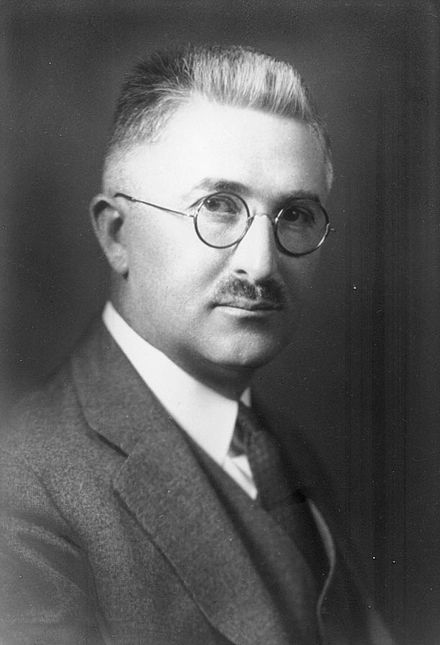
\includegraphics[width=2.7cm]{4_3_1}
\begin{center}
\footnotesize{����� ������}
\\\footnotesize{$1888 - 1970$}
\end{center}
\end{wrapfigure}

����� �������� $N$ ��������� ������� $S$ ($N$  ������ � ����������, ���������������, ����������������� ����������� �������). ���� ������ ��������� ������� ������������ ��������� ������, �� ����������� ����� $d$ ����������� ���� ������������ �� �������:

$$2^{d} \ge N \qquad \mbox{\emph{���}} \qquad  d \ge \log_{2}N$$
������, ��� ������������ �������� ������� ��������� $\log_{2}N$ ���. � ����� ������ ���������� ���������� � ������� $S$ �����:
$$H_{s} = \log_{k}N$$
������� ��������� ���������� ����������:
\begin{itemize}
  \item ��� ($k = 2$)
  \item ���� ($k = 3$)
  \item ��� (����) ($k = 10$)
  \item ��� (���) ($k = e$)
\end{itemize}
\begin{center}
\textbf{������� ������������� ���� ������}
\end{center}
\emph{\textbf{������ 1:}}
\\\emph{�������:} ������� ���������� ����� �� 1 �� 64. ����� ���������� �������� ���� "��-���" �����������, ����� �������������� ������� �����?
\\\emph{�������:}
\\$\bullet$ ������ ������: "���������� ����� ������ 32?". �����: "��".
\\$\bullet$ ������ ������: "���������� ����� ������ 16?". �����: "���".
\\ \dots
\\$\bullet$ ������ ������ ����� �������� � ����������� ������.
\\
\\������, � ������������ � ����� ������ � ������� �������� ���������� $\log_{2}64 = 6$ ��� ���������� ($N = 64$ ��� ��� �������� 64 ��������� ����������� �����).
\\�����: 6 ���.
\\
\\\emph{\textbf{������ 2:}}
\\\emph{�������:} ������� ������ �� ������ ���������� ����� � ���������� ��������� ��� �� ������������ ������ ������ �����. ����� ���������� ���������� ���������� � ��� ��������?
\\\emph{�������:} ��������� ����� ����� ������� $8\times 8$ ������. ����� ����� ���� ��� �����, ��� � ������, ������� ���������� �������������� ��������� ����� ����� $8\times 8 \times 2 = 128$. ����������, ���������� ���������� �� ���� ������ ����� $\log_{2}128 = 7$ ���.
\\�����: 7 ���.
\\���� �� ��������� $X = {x_1,x_2, ..., x_n}$ ������ ������������ �������, �� ��� ��� ���������� (�� ������) ���������� ����� �� ����� $\log_{a}n$ (������) ����������. 
\\���������� $�$ ������� �� ���������� ������������ ��������� $N$ �������, ���������� $�$ ������� �� ���������� ������������ ��������� $N$ �������.
\\
\\���� ������ �������� ���� ��� ���������, ����������� ������, ��� ��� � �������� �������� ��������� ������� ����������� ����������� (���������������).

\subsection{���� ������� }
\begin{wrapfigure}[12]{l}{2.5cm}
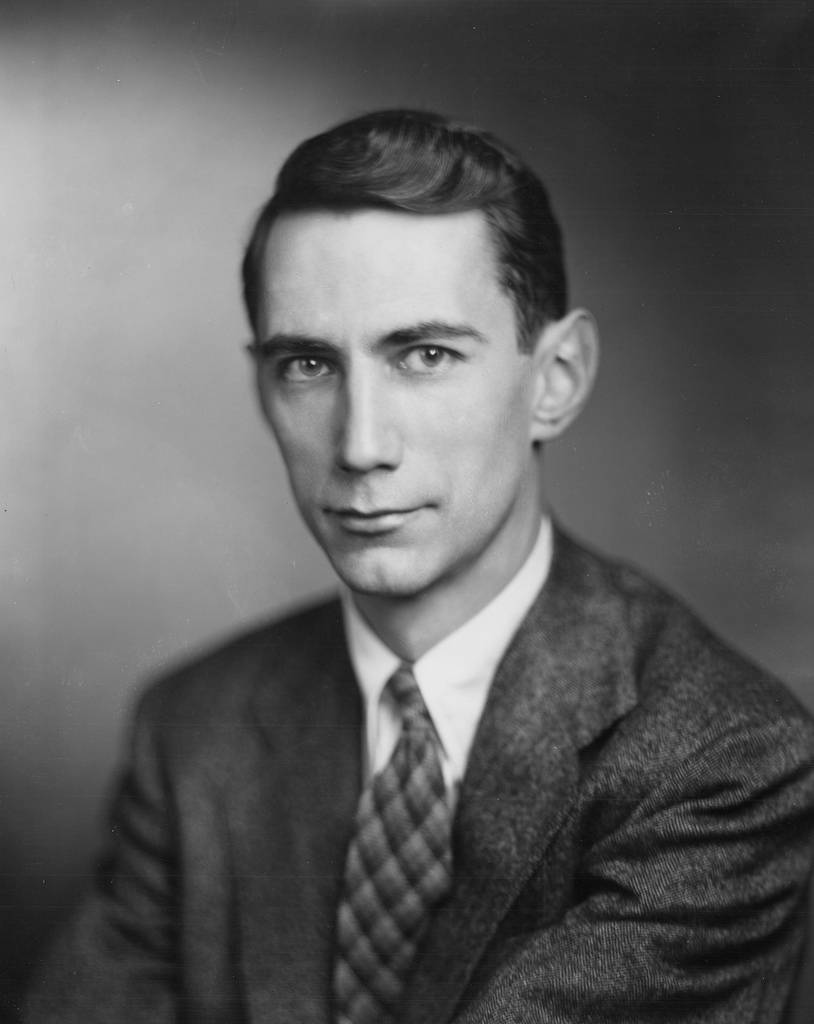
\includegraphics[width=2.5cm]{4_3_2}
\begin{center}
\footnotesize{���� ������}
\\\footnotesize{$1916 - 2001$}
\end{center}
\end{wrapfigure}

���� ��������� ������� �� �������������, ���������� ���� �������. ���� ������� ��������� ���������� ���������� �� �� ������:
$$I = - \sum^{N}_{i=1}p_{i}\times \log_{2}p_{i},$$ ���:
\\$I$ - ���������� ����������, ���������� � ����� (� $\log_{k}p_{i}$ $k = 2$);
\\$N$ - ����� ��������� �������;
\\$p_{i}$ - ����������� (������������� �������) �������� ������� � $i$-� ��������� (����������� ����, ��� ������� ��������� � ��������� $i$) \\����� ���� $p_{i}$ ������ ���� ����� �������.\\
\\���� ��� ��������� ��������������� ������� �������������, �������������, �� ���� $�_i = 1/n$ , �� �� \emph{������� �������} ����� �������� (��� ������� ������) \emph{������� ������}:
$$I = \log_{2}n.$$
\\��������� ��������:
$$f_i = -n\log_{2}p_i.$$
\newpage
����� �� \emph{������� �. �������} �������, ��� ���������� ���������� I ����� �������� ��� �������������������� ������� $f_i$ , �� ���� �������� $f_i$ ����� ���������������� ��� \emph{�������������� ���������� ������� ��������} � �������� i � ��������� $p_i$ ����������� ��������� ����� ������� � ����� ��������� (�����), ���������� ����������.\\
\\ � ������������� �������� ��� ���������� ����������� ��������� $k = 1.38 * 10^{-16} (���.����)$ � ��������� (\emph{������� ���������}) ��� �������� ��� ���� ����� � ����������������� �������:
$$ S = -k \sum^{N}_{i=1}p_{i}\times \ln{p_{i}}$$
\\ ��������� ��������� ��� I � S, ����� ���������, ��� �������� I ����� �������� ��� �������� ��-�� �������� ���������� � ������� (� �������).\\
\\������� �������� � ���������� ���������, �� ����� ������. �������� ��������� �������������� (�� ��������), ���������� � ������������� (����� ��������).\\
\\�� ���� ������� ������� ������ ������:
\begin{itemize}
\item ���������� ���� ������� ��������������� �� ���������� �������� (���������� �������) �������;
\item ���������� ���� ������� ��������������� �� ���������� �������� (���������� ����������) �������.
\end{itemize}
������������� ������� \emph{������� �������} � �� ������������� �� ������ ����������. ����� ����, � ������� �� \emph{������� ������}, ��� ��������� ����������� ���������, ��� ������ �� ��������� ��� ������������ ����������. �������� ������������� ������� \emph{������� �������} � ��� �� ���������� ��������� ��������� ������� � ���������� ������������.

\begin{center}
\textbf{������� ������������� ���� �������}
\end{center}
\emph{\textbf{������ 1:}}
\\\emph{�������:} ������� ������ ����������� �� ����� ���. ��������, ��� � ����� ����� 8 �����, �� ���: 4 �������, 2 �����, 1 ������� � 1 �����. ����� ���������� ���������� ���������� � ���� �������?
\\\emph{�������:}
\\$\bullet$ ����������� �������� ������� ��� ����� $^4/_8 = 0,5$
\\$\bullet$ ����������� �������� ����� ��� ����� $^2/_8 = 0,25$
\\$\bullet$ ����������� �������� ������� ��� ����� $^1/_8 = 0,125$
\\$\bullet$ ����������� �������� ����� ��� ����� $^1/_8 = 0,125$
\\������ ���������� ����������, ���������� � ����� �����: $I = -(0,5\hm\times \log_{2}0,5\hm + 0,25\hm\times \log_{2}0,25 + 0,125\hm\times \log_{2}0,125\hm + 0,125\hm\times \log_{2}0,125) \hm = -(-0,5\times 1 - 0,25\times 2 - 0,125\times 3 - 0,125\times 3) = -(-0,5 - 0,5\hm - 0,375\hm - 0,375\hm) = 1,75$ ���.
\\�����: 1,75 ���

\section{������ ��������� ����������}
������ ��������� ���������� ����� ������� �� ��� ������� ������:
\begin{itemize}
\item \emph{������������};
\item \emph{�������������}; 
\item \emph{��������-�������������}.
\end{itemize}
������ ���������� � �������������� ��� ��� ������ �� �����������. 
\subsection{������������ ������}
\emph{������������ ������ ��� ������ ��������� ������������ ������.}
\begin{enumerate}
\item \emph{����������} -- ���� ��������� ���������� �� �������, ��������, �������.
\item \emph{���������} -- ����������� � ����������� ������ � ����������.
\item \emph{���������} -- ����� � ������� ������������� �������� ������������ ������.
\item \emph{�����������} -- ��������������, ������������ �������, ��������, ������� � ����� ��������� �����-�� ����� �������.
\end{enumerate}
����� ������������ ���� �� ����������, � ��������� ����� ������������ �����, ��������, ������������ � ������.
\subsection{������������� ������}
\emph{������������� ������ ��� ������ ���������� ��������� ������.}
\begin{enumerate}
\item \emph{����������� �� ������������ � �����������} -- ��������� ������ � ����� ��� � ��� ������ �� ������ ������ �� ����������� ����������� � ��������, � ��������.
\item \emph{�����������} -- ��������� ������ � ����� ��� ��� ������ ����� ������������� � �������� ������ ��� ������, �� ������������ � ����������������.
\item \emph{������������} -- ��������� ������ � ����� ��� ��� ������ � ������� ������ �������������� ������������� (���������� ��������, �������������).
\item \emph{��������������} -- ��������� ������ � ����� ��� ��� ������ � ������� ��������� ������ (�� ������������ � ������ ������ �����������) � ������ ��������� �� ��� (� �� ����� ���������� �����������) ����� ������ �����������.
\item \emph{�������������} -- ��������� ������ � ����� ��� ��� ������ � ������� ������������� �����, ��������.
\end{enumerate}

\subsection{��������-������������� ������}
\emph{��������-������������� ������ (���������) ��� ������ ���������� ������ �� ������ ���������� ������������ ������ �� �������, ��������, �������.}
\begin{enumerate}
\item \emph{���������������} -- ��������� �������� ������ ��� ������������ �������, ������ ������������ �������, ��������, ������� � ������������� �������������� � ��������������.
\item \emph{������} -- ������������ ������ �� ����� � ����� ��������� �� ������.
\item \emph{������������} -- ������������ ������ �� ����� � ����������� �� ������ � ����������.
\item \emph{������} -- ���������� ������ � ����� � ����� ��������� �� ������������.
\item \emph{����������} -- ���������� ������ ������ � ����������� �� ������������ � ����������.
\item \emph{��������} -- ��������� ������ � ����� �� ������� � ������.
\item \emph{��������} -- ��������� ������ � ������ �� ������� � �����.
\item \emph{���������, ������������� ������������� ��������} -- ��������� ������ � ����� �� ������� � ������ � �� �����������, �����, ��������, �����������.
\item \emph{������������� (������� �������������)}, ������������� �������� -- ��������� ������ � ����� ��� � ��� ������ � ������� ������ ��� ��������.
\item \emph{������������ �����} -- ����� ������ � �������������� �����������, ������� �������������� ��� �� ��������.
\item \emph{���������� ����� } -- ����� ������ ����� ��������������� ������, ������ ��� ��������� � ��������.
\item \emph{�������������} -- ��������� ���������� �� ������, ������������� ������ � ����������, �� ��������� ����.
\item \emph{������������} -- ��������� ���������� � ������� �������� ������ ��� ��� ������ (� �������������, � ������) �� ������������ ��������� � ������������ ���������.
\item \emph{������������} -- ��������� ���������� � ������� ���������� ��� ����������� ������������� ��������� �������, ��������, �������.
\end{enumerate}
����� ��������� ������������ ���� ���������� ���������-������������ ������� ����� ������������ � ���������� (������� ���������� � ������� ���������), ������� ���� � ��������, ���������� ������ (���������� ����������), �������� (����������) � ������ �����.\\
\\\emph{\textbf{������ :}}
\\��� ���������� ������ ������������ � ���������� ������������� � ������ ������, ������� ��� ������� ������� ����� ������ ��������� ��������:
\begin{enumerate}
\item ���������� ����������� �����, ������ ���������� � �������� �������, �������; ��� ���� ���� ������������ ������ ����������, ���������, ���������, ������������, ������� � �������, �������� � ��������, �������������, ������������ � ���������� ������, ������������� � ��.;
\item ���������� ��������, ����, ��������� �������� ������������; �������� ������������ ������ � ����������, ���������, �����������, ���������������, ������, ������, ��������, ��������, �������������, ������������, ���������� � ��.;
\item ��������������� ������������ �������; �������� ������������ ������ � ���������������, ������, ������, ��������, ��������, ������������, ����������� � ��.;
\item ����� ������� �������� ������������ � ������� ��������� ���������, �������� ������������, ����� ������������ �������; ������������ ���� ������ � ���������, ���������, �����������, ������, ������, ��������, ��������, ������������, �������������, ������������, ������������� � ��.
\end{enumerate}

\chapter{Сжатие данных}
\textbf{Сжатие данных} - это процесс, обеспечивающий уменьшение объема данных путем сокращения их избыточности.
\begin{flushright}
  К. Шеннон
\end{flushright}
\parКлода Шеннона принято считать основоположником науки о сжатии информации. Его теорема об оптимальном кодировании показывает, к чему нужно стремиться при кодировании информации и насколько та или иная информация при этом сожмется. Кроме того, им были проведены опыты по эмпирической оценке избыточности английского текста. Шенон предлагал людям угадывать следующую букву и оценивал вероятность правильного угадывания. На основе ряда опытов он пришел к выводу, что количество информации в английском тексте колеблется в пределах 0,6 – 1,3 бита на символ. Несмотря на то, что результаты исследований Шеннона были по-настоящему востребованы лишь десятилетия спустя, трудно переоценить их значение.\\
\\\emph{Сжатие данных} -- это частный случай \emph{кодирования} данных и важнейший аспект передачи данных, который дает возможность более оперативно передавать данные. 
\\\\\emph{Цель сжатия} -- уменьшение количества бит, необходимых для хранения или передачи заданной информации. Это дает возможность передавать сообщения более быстро и хранить более экономно и оперативно (последнее означает, что операция извлечения данной информации с устройства ее хранения будет проходить быстрее, что возможно, если скорость распаковки данных выше скорости считывания данных с носителя информации).\\
\\Сжатие позволяет, например, записать больше информации на дискету, "увеличить" размер жесткого диска, ускорить работу с модемом и т.д. При работе с компьютерами широко используются программы-архиваторы данных формата ZIP, GZ, ARJ и других. Методы сжатия информации были разработаны как математическая теория, которая долгое время (до первой половины 80-х годов), мало использовалась в компьютерах на практике.\\
\\Введем ряд определений, которые будут использоваться далее в изложении материала.
\\\textbf{Алгоритм сжатия данных (алгоритм архивации)} -- это алгоритм, который устраняет избыточность записи данных.
\\\textbf{Символ} -- наименьшая единица данных, рассматриваемая как единое целое при кодировании/декодировании.
\\\textbf{Алфавит} -- множество всех возможных символов. При сжатии англоязычных текстов обычно используют множество из 128 ASCII кодов. При сжатии изображений множество значений пиксела может содержать 2, 16, 256 или другое количество элементов.
\\
\\Рассмотрим на примере. Возьмем обычную книгу и будем считать ее содержимое как за исходные данные. За символ мы можем взять как букву (и тогда алфавитом будет являться обычный алфавит русского языка), так и целое слово (тогда алфавит будет состоять из всех уникальных слов, встречающихся в этой книге). Символ - не обязательно один знак. Символом могут являться слова и даже целые предложения.\\
\\\textbf{Токен} -- единица данных, записываемая в сжатый поток некоторым алгоритмом сжатия. Токен состоит из нескольких полей фиксированной или переменной длины.
\\\textbf{Фраза} -- фрагмент данных, помещаемый в словарь для дальнейшего использования в сжатии.
\\\textbf{Код} -- правило соответствия набора знаков одного множества $X$ знакам другого множества $Y$.
\\\textbf{Кодирование} -- процесс преобразования символов алфавита $Х$ в символы алфавита $Y$.
\\\textbf{Декодирование} -- процесс, обратный кодированию, при котором осуществляется восстановление данных.
\\\textbf{Кодовый символ} -- наименьшая единица данных, подлежащая сжатию. Обычно символ – это 1 байт, но он может быть битом, тритом {0,1,2}, или чем-либо еще.
\\\textbf{Кодовое слово} -- это последовательность кодовых символов из алфавита кода.
\\\textbf{Средняя длина кодового слова} - это величина, которая вычисляется как взвешенная вероятностями сумма длин всех кодовых слов.
\\То есть:
$$ L = \sum_{i=1}^{N}p_{i}\times l_{i},$$ где: 
\\$N$ - количество кодовых слов в алфавите;
\\$p_{i}$ - вероятность появления кодового слова в последовательности;
\\$l_{i}$ - количество символов в кодовом слове (длина кодового слова).
\\Сумма всех $p_{i}$ должна быть равна единице.
\\
\\Если все кодовые слова имеют одинаковую длину, то код называется \textbf{равномерным} (фиксированной длины). Если встречаются слова разной длины, то - \textbf{неравномерным} (переменной длины).
\\
\\Классический пример равномерного кода - таблица символов ASCII. Любой символ из этой таблицы будет закодирован одним байтом (один символ всегда кодируется двумя цифрами в шестнадцатеричной системе счисления).
\\Пример неравномерного кода - азбука Морзе.
\\
\begin{center}
  \textbf{Характеристики кодирования}
\end{center}
\begin{table}[h]
\begin{center}
\begin{tabular}{c c c}
\multirow{2}{*}{Коэффициент сжатия} & \multirow{2}{*}{ = }  & Размер входного потока  \\
\hhline{~~-}
 &  & Размер выходного потока
\end{tabular}
\end{center}
Значения больше 1 обозначают сжатие, а значения меньше 1 – расширение.
\end{table}
\begin{table}[h]
\begin{center}
\begin{tabular}{c c c}
\multirow{2}{*}{Отношение сжатия} & \multirow{2}{*}{ = }  & Размер выходного потока  \\
\hhline{~~-}
 &  & Размер входного потока
\end{tabular}
\end{center}
Значение 0,6 означает, что данные занимают 60\% от первоначального объема. Значения больше 1 означают, что выходной поток больше входного (отрицательное сжатие, или расширение).
\end{table}

Сжатие данных можно разделить на два основных типа:
\begin{itemize}
\item \textbf{Сжатие без потерь} (\emph{полностью обратимое}) - это метод сжатия данных, при котором ранее закодированная порция данных восстанавливается после их распаковки полностью без внесения изменений. Для каждого типа данных, как правило, существуют свои оптимальные алгоритмы сжатия без потерь;
\item \textbf{Сжатие с потерями} (\emph{частично обратимое}) -  это метод сжатия данных, при котором для обеспечения максимальной степени сжатия исходного массива данных часть содержащихся в нем данных отбрасывается. Для текстовых, числовых и табличных данных использование программ, реализующих подобные методы сжатия, является неприемлемыми. В основном такие алгоритмы применяются для сжатия аудио- и видеоданных, статических изображений.
\end{itemize}
Существуют два основных способа проведения сжатия:
\begin{itemize}
\item \textbf{Статические методы} -- методы сжатия, присваивающие коды переменной длины символам входного потока, причем более короткие коды присваиваются символам или группам символам, имеющим большую вероятность появления во входном потоке. Лучшие статистические методы применяют кодирование Хаффмана.
\item \textbf{Словарное сжатие} -- это методы сжатия, хранящие фрагменты данных в <<словаре>> (некоторая структура данных). Если строка новых данных, поступающих на вход, идентична какому-либо фрагменту, уже находящемуся в словаре, в выходной поток помещается указатель на этот фрагмент. Важно заметить, что иногда словарь может передаваться в начале самого сообщения.
\end{itemize}

\textbf{Префиксный код} -- это код, в котором никакое кодовое слово не является префиксом любого другого кодового слова. Эти коды имеют переменную длину.
\\
\\\textbf{Оптимальный префиксный код} -- это префиксный код, имеющий минимальную среднюю длину.
\\
\newpage
\section{Алгоритмы сжатия данных}
\subsection{Алгоритм Шеннона-Фано}
\begin{wrapfigure}[13]{l}{3cm}
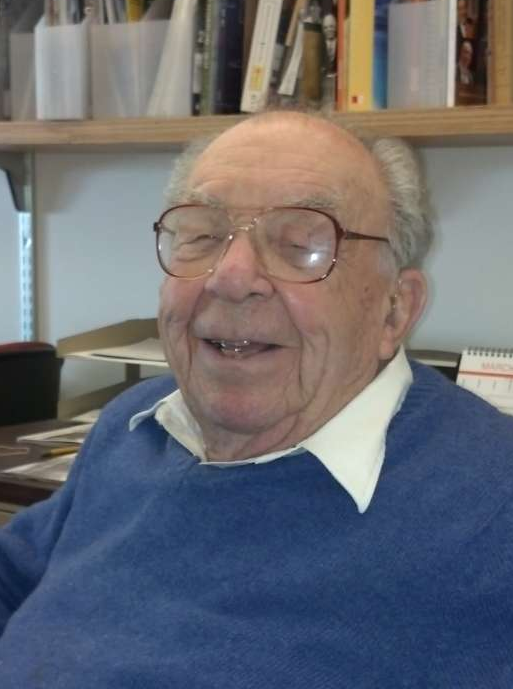
\includegraphics[width=3cm]{5_1}
\begin{center}
\caption{}
\footnotesize{Роберт Фано}
\\\footnotesize{$\mbox{род.} 1917$}
\end{center}
\end{wrapfigure}
Алгоритм Шеннона-Фано - один из первых алгоритмов сжатия. Его сформулировали два ученых - Клод Шеннон и Роберт Фано. Алгоритм основан на частоте повторения. Так, часто встречающийся символ кодируется кодом меньшей длины, а редко встречающийся - кодом большей длины.
Коды, полученные при кодировании, префиксные, что позволяет декодировать любую последовательность.
\\
\\Алгоритм Шеннона-Фано для некоторых последовательностей может сформировать неоптимальные коды.
\\
\begin{center}
\textbf{Алгоритм Шеннона-Фано}
\end{center}

\begin{enumerate}
\item Символы входного (первичного) алфавита выписывают по убыванию вероятностей - это корень будущего дерева.
\item Строится дерево от корня к листьям. Находится середина, которая делит корень на два узла. Эти узлы (суммы вероятностей символов алфавита) примерно равны.
\item Полученные узлы - листья дерева. Левому узлу (с большей суммарной вероятностью) присваивается значение $1$, а правому - $0$.
\item Шаги 2-3 повторяются, пока в листьях дерева не останется один символ первичного алфавита.
\item Символ входного (первичного) алфавита кодируется последовательностью нулей и единиц в соответствии с распределением их от корня к листьям (узлам).
\end{enumerate}
\emph{\textbf{Пример 1:}}
\\\emph{Задание:} составить код Шеннона-Фано для последовательности
\\$AAABCCCCCDEEEF$. Найти среднюю длину кодового слова.
\\\emph{Решение:} в последовательности AAABCCCCCDEEEF алфавит состоит из 6 символов: A, B, C, D, E, F. Выпишем символы первичного алфавита по убыванию вероятностей:
\\$\bullet$ Вероятность символа $C$ - $^5/_{14}$;
\\$\bullet$ Вероятность символа $A$ - $^3/_{14}$;
\\$\bullet$ Вероятность символа $E$ - $^3/_{14}$;
\\$\bullet$ Вероятность символа $B$ - $^1/_{14}$;
\\$\bullet$ Вероятность символа $D$ - $^1/_{14}$;
\\$\bullet$ Вероятность символа $F$ - $^1/_{14}$.
\\Полученная последовательность $CAEDBF$ является корнем будущего дерева.
\\Построим дерево от корня к листьям:
\begin{table}[h]
\centering
\begin{tabular}{c c c c c c}
\multicolumn{6}{c}{CAEBDF ($^5/_{14} + ^3/_{14} + ^3/_{14} + ^1/_{14} + ^1/_{14} + ^1/_{14}$)} \\
\multicolumn{2}{c}{$\downarrow$} & \multicolumn{4}{c}{$\downarrow$} \\
\multicolumn{2}{c}{CA ($^5/_{14} + ^3/_{14}$)} & \multicolumn{4}{c}{EBDF ($^3/_{14} + ^1/_{14} + ^1/_{14} + ^1/_{14}$)} \\
$\downarrow$ & $\downarrow$ & \multicolumn{2}{c}{$\downarrow$} & \multicolumn{2}{c}{$\downarrow$} \\
C ($^5/_{14}$) & A ($^3/_{14}$) & \multicolumn{2}{c}{EB ($^3/_{14} + ^1/_{14}$)} & \multicolumn{2}{c}{DF ($^1/_{14} + ^1/_{14}$)} \\
 & & $\downarrow$ & $\downarrow$ & $\downarrow$ & $\downarrow$ \\
 & & E ($^3/_{14}$) & B ($^1/_{14}$) & D ($^1/_{14}$) & F($^1/_{14}$) \\
\end{tabular}
\end{table}
\\Присвоим левому символу (с большей вероятностью) значение $1$, а правому - $0$:
\begin{table}[h]
\centering
\begin{tabular}{c c c c c c}
\multicolumn{6}{c}{CAEBDF ($^5/_{14} + ^3/_{14} + ^3/_{14} + ^1/_{14} + ^1/_{14} + ^1/_{14}$)} \\
& $\downarrow$ & \multicolumn{4}{c}{$\downarrow$} \\
\multicolumn{2}{c}{CA ($^5/_{14} + ^3/_{14}$) [1]} & \multicolumn{4}{c}{EBDF ($^3/_{14} + ^1/_{14} + ^1/_{14} + ^1/_{14}$) [0]} \\
$\downarrow$ & $\downarrow$ & \multicolumn{2}{c}{$\downarrow$} & \multicolumn{2}{c}{$\downarrow$} \\
C ($^5/_{14}$) [1] & A ($^3/_{14}$) [0] & \multicolumn{2}{c}{EB ($^3/_{14} + ^1/_{14}$) [1]} & \multicolumn{2}{c}{DF ($^1/_{14} + ^1/_{14}$) [0]} \\
 & & $\downarrow$ & $\downarrow$ & $\downarrow$ & $\downarrow$ \\
 & & E ($^3/_{14}$) [1] & B ($^1/_{14}$) [0] & D ($^1/_{14}$) [1] & F($^1/_{14}$) [0] \\
\end{tabular}
\end{table}
\\
\\Получим следующую таблицу для кодировки:
\begin{table}[h]
\begin{tabular}{|c|c|c|}
\hline
Символ & Вероятность & Код \\
\hline
C & $^5/_{14}$ & 11 \\
A & $^3/_{14}$ & 10 \\
E & $^3/_{14}$ & 011 \\
B & $^1/_{14}$ & 010 \\
D & $^1/_{14}$ & 001 \\
F & $^1/_{14}$ & 000 \\
\hline
\end{tabular}
\end{table}
\\Исходная последовательность AAABCCCCCDEEEF кодируется следующей: $10.10.10.010.11.11.11.11.11.001.011.011.011.000 - 34$ бита.
\\Средняя длина кодового слова: $^5/_{14}\times 2 + ^3/_{14}\times 2 + ^3/_{14}\times 3 + ^1/_{14}\times 3\hm + ^1/_{14}\hm\times 3\hm + ^1/_{14}\hm\times 3\hm = ^{34}/_{14} \approx 2,4.$
\subsection{Код Хаффмана}
\begin{wrapfigure}[14]{l}{3cm}
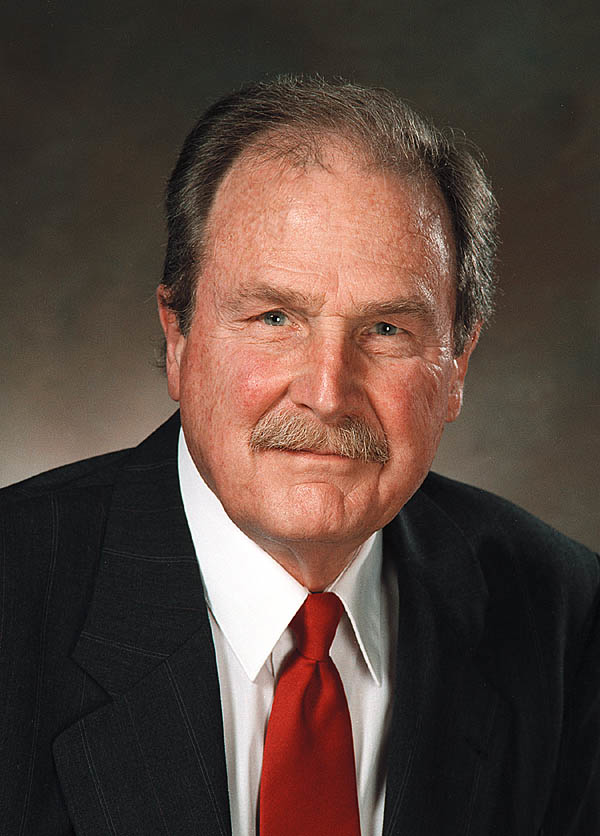
\includegraphics[width=3cm]{5_2}
\begin{center}
\caption{}
\footnotesize{Дэвид Хаффман}
\\\footnotesize{$1925 - 1999$}
\end{center}
\end{wrapfigure}
Код (алгоритм) Хаффмана был разработан в 1952 году аспирантом Массачусетского технологического института Дэвидом Хаффманом при написании им курсовой работы.
\\Как и алгоритм Шеннона-Фано, основан на частоте повторения. Зная вероятности символов в сообщении, можно описать процедуру построения кодов переменной длины, состоящих из целого количества битов. Символам с большей вероятностью ставятся в соответствие более короткие коды. Коды Хаффмана обладают свойством префиксности, что позволяет однозначно их декодировать.
\\Однако, в отличие от кодов Шеннона-Фано, коды Хаффмана всегда являются оптимальными.
\\Сжатие данных по Хаффману применяется при сжатии фото- и видеоизображений (JPEG, стандарты сжатия MPEG), в архиваторах (PKZIP, LZH), в протоколах передачи данных MNP5 и MNP7.
\begin{center}
  \textbf{Алгоритм Хаффмана для неоптимальных префиксных кодов}
\end{center}

\begin{enumerate}
  \item Символы входного алфавита образуют список свободных узлов. Каждый узел имеет вес, равный вероятности появления символа в сжимаемом тексте (исходной последовательности). Строится дерево от листьев (узлов) к корню.
  \item Выбираются два свободных узла дерева с наименьшими весами.
  \item Создается их родитель с весом, равным их суммарному весу.
  \item Родитель добавляется в список свободных узлов, а двое его детей удаляются из этого списка.
  \item Одной дуге, выходящей из родителя (узлу с большим весом), ставится в соответствие значение $1$, а другой (узлу с меньшим весом) значение $0$.
  \item Повторяем шаги 2-4, выбирая в качестве одного из свободных узлов родителя, до тех пор, пока в списке свободных узлов не останется только один свободный узел. Он и будет считаться корнем дерева.
  \item Символ входного (первичного) алфавита кодируется последовательностью нулей и единиц в соответствии с распределением их от корня дерева к узлам (листьям).
\end{enumerate}

\emph{\textbf{Пример 1:}}
\\\emph{Задание:} составить код Хаффмана для неоптимальных префиксных кодов для последовательности AAABCCCCCDEEEF. Найти среднюю длину кодового слова.
\\\emph{Решение:} составим список свободных узлов для исходной последовательности:
\\$\bullet$ Символ $A$ с вероятностью $^3/_{14}$;
\\$\bullet$ Символ $B$ с вероятностью $^1/_{14}$;
\\$\bullet$ Символ $C$ с вероятностью $^5/_{14}$;
\\$\bullet$ Символ $D$ с вероятностью $^1/_{14}$;
\\$\bullet$ Символ $E$ с вероятностью $^3/_{14}$;
\\$\bullet$ Символ $F$ с вероятностью $^1/_{14}$.
\\Построим кодовое дерево:
\begin{table}[h]
\centering
\begin{tabular}{c c c c c c}
\multicolumn{6}{l}{DBFAEC ($^1/_{14} + ^1/_{14} + ^1/_{14} + ^3/_{14} + ^3/_{14} + ^5/_{14}$)} \\
$\downarrow$ & \multicolumn{5}{c}{$\downarrow$} \\
C ($^5/_{14}$) & \multicolumn{5}{l}{DBFAE ($^1/_{14} + ^1/_{14} + ^1/_{14} + ^3/_{14} + ^3/_{14}$)} \\
& $\downarrow$ & \multicolumn{4}{c}{$\downarrow$} \\
& E ($^3/_{14}$) & \multicolumn{4}{l}{DBFA ($^1/_{14} + ^1/_{14} + ^1/_{14} + ^3/_{14}$)} \\
& & $\downarrow$ & \multicolumn{3}{c}{$\downarrow$} \\
& & A ($^3/_{14}$) & \multicolumn{3}{l}{DBF ($^1/_{14} + ^1/_{14} + ^1/_{14}$)} \\
& & & $\downarrow$ & \multicolumn{2}{c}{$\downarrow$} \\
& & & F ($^1/_{14}$) & \multicolumn{2}{l}{DB ($^1/_{14} + ^1/_{14}$)} \\
& & & & $\downarrow$ & $\downarrow$ \\
& & & & B ($^1/_{14}$) & D ($^1/_{14}$) \\
\end{tabular}
\end{table}
\\Одной дуге, выходящей из родителя (узлу с большим весом), присвоим значение $1$, а другой (узлу с меньшим весом) - значение $0$.
\begin{table}[h]
\centering
\begin{tabular}{c c c c c c}
\multicolumn{6}{l}{DBFAEC ($^1/_{14} + ^1/_{14} + ^1/_{14} + ^3/_{14} + ^3/_{14} + ^5/_{14}$)} \\
$\downarrow$ & \multicolumn{5}{l}{$\downarrow$} \\
C ($^5/_{14}$) [0] & \multicolumn{5}{l}{DBFAE ($^1/_{14} + ^1/_{14} + ^1/_{14} + ^3/_{14} + ^3/_{14}$) [1]} \\
& $\downarrow$ & \multicolumn{4}{l}{$\downarrow$} \\
& E ($^3/_{14}$) [0] & \multicolumn{4}{l}{DBFA ($^1/_{14} + ^1/_{14} + ^1/_{14} + ^3/_{14}$) [1]} \\
& & $\downarrow$ & \multicolumn{3}{l}{$\downarrow$} \\
& & A ($^3/_{14}$) [0] & \multicolumn{3}{l}{DBF ($^1/_{14} + ^1/_{14} + ^1/_{14}$) [1]} \\
& & & $\downarrow$ & \multicolumn{2}{l}{$\downarrow$} \\
& & & F ($^1/_{14}$) [0] & \multicolumn{2}{l}{DB ($^1/_{14} + ^1/_{14}$) [1]} \\
& & & & $\downarrow$ & \multicolumn{1}{c}{$\downarrow$} \\
& & & \multicolumn{3}{l}{\qquad B ($^1/_{14}$) [0] \qquad D ($^1/_{14}$) [1]}\\
\end{tabular}
\end{table}
\\
\\
\\Получим следующую таблицу для кодировки:
\\
\begin{table}[h]
\begin{tabular}{|c|c|}
\hline
Символ &  Код \\
\hline
A & 110 \\
B & 11110 \\
C & 0 \\
D & 11111 \\
E & 10 \\
F & 1110 \\
\hline
\end{tabular}
\end{table}
\\Исходная последовательность AAABCCCCCDEEEF кодируется следующей: $110.110.110.11110.0.0.0.0.0.11111.10.10.10.1110$ - 34 бита.
\\Средняя длина кодового слова: $^5/_{14}\times 1 + ^3/_{14}\times 2 + ^3/_{14}\times 3 + ^1/_{14}\times 4\hm + ^1/_{14}\hm\times 5\hm + ^1/_{14}\hm\times 5\hm = ^{34}/_{14} \approx 2,4.$
\begin{center}
  \textbf{Алгоритм Хаффмана для оптимальных префиксных кодов}
\end{center}

\begin{enumerate}
  \item Символы входного (первичного) алфавита выписывают по убыванию вероятностей (весов) в таблицу.
  \item Выбираются два свободных узла (элемента) с наименьшими весами (вероятностями).
  \item Верхнему узлу (с большим весом) присваивается значение $1$, а нижнему (с меньшим весом) - $0$.
  \item Создается их родитель с весом, равным их суммарному весу.
  \item Родитель добавляется в список свободных узлов (таблицу), занимая соответствующее место в списке убывающих во величине весов (вероятностей), а двое его детей удаляются из этого списка.
  \item Повторяем шаги 2-5, до тех пор, пока в списке свободных узлов (в таблице) не останется только два свободных узла (элемента).
  \item Символ входного (первичного) алфавита кодируется последовательностью нулей и единиц в соответствии с распределением их от корня к узлам.
\end{enumerate}

\emph{\textbf{Пример 2:}}
\\\emph{Задание:} составить код Хаффмана для неоптимальных префиксных кодов для последовательности AAABCCCCCDEEEF. Найти среднюю длину кодового слова.
\\\emph{Решение:} составим список свободных узлов для исходной последовательности:
\\
\begin{minipage}[h]{\textwidth}
\begin{tabular}{|c|c|}
\hline
Символ &  Вероятность, p \\
\hline
C & $^5/_{14}$ \\
A & $^3/_{14}$ \\
E & $^3/_{14}$ \\
B & $^1/_{14}$ \\
D & $^1/_{14}$ \\
F & $^1/_{14}$ \\
\hline
\end{tabular}
\end{minipage}
\\ \\
\\Построим таблицу:
\\
\\\begin{minipage}[h]{\textwidth}
\begin{tabular}{|c|c||c|c||c|c||c|c||c|c|}
\hline
C & $^5/_{14}$ & C & $^5/_{14}$ & C & $^5/_{14}$ & EDFB & $^6/_{14}$ & CA & $^8/_{14}$ \\
A & $^3/_{14}$ & A & $^3/_{14}$ & A & $^3/_{14}$ & C & $^5/_{14}$ & EDFB & $^6/_{14}$ \\
E & $^3/_{14}$ & E & $^3/_{14}$ & E & $^3/_{14}$ & A & $^3/_{14}$ & & \\
B & $^1/_{14}$ & DF & $^2/_{14}$ & DFB & $^3/_{14}$ & & & &\\
D & $^1/_{14}$ & B & $^1/_{14}$ & & & & & &\\
F & $^1/_{14}$ & & & & & & & &\\
\hline
\end{tabular}
\end{minipage}
\\
\\Верхнему узлу (с большим весом) присвоим значение $1$, а нижнему (с меньшим весом) - $0$:
\begin{table}[h]
\begin{tabular}{|c|c||c|c||c|c||c|c|}
\hline
C & $^5/_{14}$ & C & $^5/_{14}$ & C & $^5/_{14}$ & EDFB & $^6/_{14}$   \\
A & $^3/_{14}$ & A & $^3/_{14}$ & A & $^3/_{14}$ & C [1] & $^5/_{14}$   \\
E & $^3/_{14}$ & E & $^3/_{14}$ & E [1] & $^3/_{14}$ & A [0] & $^3/_{14}$  \\
B & $^1/_{14}$ & DF [1] & $^2/_{14}$ & DFB [0] & $^3/_{14}$ & & \\
D [1] & $^1/_{14}$ & B [0] & $^1/_{14}$ & & & & \\
F [0] & $^1/_{14}$ & & & & & & \\
\hline
\end{tabular}
\end{table}
\\
\begin{minipage}[h]{6cm}
\begin{tabular}{|c|c|}
\hline
CA [1] & $^8/_{14}$ \\
EDFB [0] & $^6/_{14}$ \\
& \\
& \\
& \\
& \\
\hline
\end{tabular}
\end{minipage}
\\\\\\\\\\\\\\\\\\\\\\
\\Построим кодовое дерево:\\
\\
\begin{minipage}[!h]{\textwidth}
\centering
\begin{tabular}{c c c c c c}
\multicolumn{6}{c}{CAEDFB ($^5/_{14} + ^3/_{14} + ^3/_{14} + ^1/_{14} + ^1/_{14} + ^1/_{14}$)} \\
\multicolumn{2}{c}{$\downarrow$} & \multicolumn{4}{c}{$\downarrow$} \\
\multicolumn{2}{c}{CA ($^5/_{14} + ^3/_{14}$) [1]} & \multicolumn{4}{c}{EDFB ($^3/_{14} + ^1/_{14} + ^1/_{14} + ^1/_{14}$) [0]} \\
$\downarrow$ & $\downarrow$ & \qquad $\downarrow$ & \multicolumn{3}{c}{$\downarrow$} \\
C ($^5/_{14}$) [1] & A ($^3/_{14}$) [0] & E ($^3/_{14}$) [1] & \multicolumn{3}{c}{DFB ($^1/_{14} + ^1/_{14} + ^1/_{14}$) [0]} \\
& & & \multicolumn{2}{c}{$\downarrow$} & $\downarrow$ \\
& & & \multicolumn{2}{r}{DF ($^1/_{14} + ^1/_{14}$) [1]} & B ($^1/_{14}$) [0] \\
\multicolumn{5}{r}{$\downarrow$ \qquad \qquad $\downarrow$ \qquad \qquad} & \\
\multicolumn{5}{r}{D ($^1/_{14}$) [1] \qquad  F ($^1/_{14}$) [0]} & \\
\end{tabular}
\end{minipage}
\\
\\
\\Получим следующую таблицу для кодировки:
\begin{table}[h]
\begin{tabular}{|c|c|}
\hline
Символ &  Код \\
\hline
A & 10 \\
B & 000 \\
C & 11 \\
D & 0011 \\
E & 01 \\
F & 0010 \\
\hline
\end{tabular}
\end{table}
\\Исходная последовательность AAABCCCCCDEEEF кодируется следующей: $10.10.10.000.11.11.11.11.11.0011.01.01.01.0010$ - 33 бита.
\\Средняя длина кодового слова: $^5/_{14}\times 2 + ^3/_{14}\times 2 + ^3/_{14}\times 2 + ^1/_{14}\times 3\hm + ^1/_{14}\hm\times 4\hm + ^1/_{14}\hm\times 4\hm = ^{33}/_{14} \approx 2,35.$
Классический алгоритм Хаффмана имеет один существенный недостаток. Для восстановления содержимого сжатого текста при декодировании необходимо знать таблицу частот, которую использовали при кодировании. Следовательно, длина сжатого текста увеличивается на длину таблицы частот, которая должна посылаться впереди данных, что может свести на нет все усилия по сжатию данных. Кроме того, необходимость наличия полной частотной статистики перед началом собственно кодирования требует двух проходов по тексту: одного для построения модели текста (таблицы частот и дерева Хаффмана), другого для собственно кодирования.\\

\subsection{Кодирование длин серий}
\emph{\textbf{Кодирование длин серий (кодирование повторов)}} - алгоритм сжатия данных, заменяющий повторяющиеся символы (серии) на один символ и число его повторов. \emph{\textbf{Серией}} называется последовательность, состоящая из нескольких одинаковых символов. При кодировании (упаковке, сжатии) строка одинаковых символов, составляющих серию, заменяется строкой, содержащей сам повторяющийся символ и количество его повторов.
\\Кодирование длин серий активно применяется при сжатии графических изображений, таких как иконки или графические изображения.
\\
\\\emph{\textbf{Пример :}}
\\\emph{Задание:} применить кодирование длин серий для последовательности \\$AAAAABAAAAABBBBBAAAAA$.
\\\emph{Решение:} посчитаем количество повторяющихся символов:
\\$1.$ $5$ символов $A$;
\\$2.$ $1$ символ $B$;
\\$3.$ $5$ символов $A$;
\\$4.$ $5$ символов $B$;
\\$5.$ $5$ символов $A$.
\\Итого, найдено 5 серий. Заменим серии на число повторов и сам повторяющийся символ: $5A1B5A5B5A$. Получилась последовательность из 10 символов. Исходная последовательность состояла из 21 символа.
\\Коэффициент сжатия: $\frac{21}{10} = 2,1$.

\subsection{Метод относительного кодирования}
В некоторых случаях информация может состоять из блоков данных, каждый из которых может немного отличаться от предыдущего. Примером могут служить последовательные кадры видеоизображения. Для таких случаев используется метод относительного кодирования. Данный подход предполагает запись отличий, существующих между последовательными блоками данных, вместо записи самих этих блоков, т.е. каждый блок кодируется с точки зрения его взаимосвязи с предыдущим блоком. 
\\\emph{\textbf{Пример :}}
\\\emph{Задание:} применить метод относительного кодирования для последовательности чисел \\$1476; 1473; 1480; 1477$.
\\\emph{Решение:} Берем изначально число 1476, смещение до 1473 относительно него равно -3, смещение до 1480 относительно второго числа равно +7; т.о. представим последовательность в следующем виде: 1476; -3; +7; -3.

\subsection{Частотно-зависимое кодирование}
Этот метод сжатия данных предполагает применение частотно-зависимого кодирования, при котором длина битовой комбинации, представляющей элемент данных, обратно пропорциональна частоте использования этого элемента. Такие коды входят в группу кодов переменной длины, т.е. элементы данных в этих кодах представляются битовыми комбинациями различной длины. Если взять английский текст, закодированный с помощью частотно-зависимого метода, то чаще всего встречающиеся символы [e, t, a, i] будут представлены короткими битовыми комбинациями, а те знаки, которые встречаются реже [z, q, x], - более длинными битовыми комбинациями. В результате мы получим более короткое представление всего текста, чем при использовании обычного кода, подобного Unicode или ASCII. Построение алгоритма, который обычно используется при разработке частотно-зависимых кодов, приписывают Девиду Хаффмануу, поэтому такие коды часто называют кодами Хаффмана.\\
\\\emph{\textbf{Пример :}}
\\\emph{Задание:} требуется закодировать частотно-зависимым методом последовательность:\\ $$\alpha\gamma\alpha\alpha\beta\alpha\alpha\gamma\alpha\alpha\beta\alpha\lambda\alpha\alpha\beta\alpha\beta\alpha\beta\alpha\beta\alpha\alpha,$$
\\\emph{Решение:} последовательность состоит из четырех символов $\alpha, \beta, \gamma$ и $\lambda$. Причем в ней $\alpha$ встречается 15 раз, $\beta$ -- 6 раз, $\gamma$ -- 2 раза и $\lambda$ - 1 раз.\\
Выберем в соответствии с методом Хаффмана следующий двоичный код для представления символов:\\
\\$\alpha - 1$
\\$\beta - 01$
\\$\gamma - 001$
\\$\lambda - 000$\\
\\Получим в итоге последовательность: 100111011100111011000110110110110111.
\subsection{Метод Лемпеля-Зива}
Данный метод назван в честь его создателей, Абрахама Лемпеля и Джекоба Зива. Системы кодирования по методу Лемпеля-Зива используют технологию кодирования с применением адаптивного словаря, эта система используется при создании сжатых файлов, называемых zip – файлами. В текущем контексте словарем является набор стандартных блоков,  из которых построено сообщение, которое нужно сжать. Если бы мы хотели сжать текст на английском алфавите, то такими стандартными блоками были бы буквы алфавита. Если бы мы хотели сжать уже закодированные данные, то стандартными блоками были бы цифры 0 и 1. При адаптивном кодировании словарь может изменяться в процессе кодирования.\\
\\В качестве примера рассмотрим алгоритм \textbf{LZ77} – частный случай алгоритма Лемпеля-Зива.\\
Начнем с простого цитирования начальной части сообщения. Затем представим оставшуюся часть сообщения в виде последовательности троек (содержащих два целых числа, за которыми следует символ из сообщения). Каждая такая тройка описывает, как должна строиться следующая часть сообщения на основе предыдущей. Следовательно, словарь, из которого строится сообщение, состоит из самого сообщения.\\
\\\emph{\textbf{Пример :}}
\\\emph{Задание:} дано сжатое сообщение xyxxyzy(5,4,x), необходимо развернуть сообщение так, чтобы получить исходную последовательность.
\\\emph{Решение:} сообщение xyxxyzy(5,4,x) состоит из начального сегмента xyxxyzy, за которым следует тройка (5,4,x).
Чтобы развернуть оставшуюся часть сообщения, необходимо расшифровать тройку (5,4,x). Первое число тройки показывает, на сколько символов нужно вернуться назад в развернутой цепочке.
$$xy\downarrow xxyzy$$
 Далее нужно добавить в конец развернутой цепочки символы, находящиеся в этой позиции. Второе число показывает, сколько символов нужно добавлять.
$$xy\downarrow \textbf{xxyz}y$$
$$xyxxyzyxxyz$$
В завершение добавляем в конец цепочки последний символ тройки.
$$xyxxyzyxxyzx$$
Для того чтобы сжать сообщение с помощью алгоритма LZ77, сначала переписываем начальный сегмент сообщения, затем в этом сегменте ищем самую длинную цепочку, которая совпадает с оставшейся частью сообщения. К этой цепочке будет относиться первая тройка. 
\subsection{Сжатие изображений}
Растровые изображения представляются обычно 3 байта на один пиксел, это приводит к большим и трудно обрабатываемым файлам растровой графики. Для того, чтобы уменьшить требования к памяти, было разработано много схем сжатия изображений. Одна из них, разработанная компанией CompuServe, называется GIF(Graphic Interchange Format - формат графического обмена). Этот стандарт сжатия решает проблему, сокращая количество цветов, которые могут быть приписаны пикселу, до 256. Это позволяет представить значение каждого пиксела спомощью одного байта вместо трех. Каждому коду при помощи таблицы (палитры) ставится в соответствие определенное сочетание красного, синего и зеленого цветов. Одному из цветов используется значение «прозрачный», то есть через любой участок изображения, которому присвоен этот цвет, виден фон. Эта возможность и простота формата обусловили его широкое использование в компьютерных играх, где многочисленные изображения перемещаются по экрану.\\
\\Другой стандарт сжатия изображений -- JPEG (разработан Joint Photo- graphic Experts Group - объединенной группой экспертов в области фотографии) принят производителями цифровых камер для цифровых фотографий. Стандарт JPEG включает в себя несколько способов представления изображения, у каждого из которых своя задача.\\
\\Когда требуется предельная точность, используется метод «без потерь», при котором хранится различие между соседними пикселами, а не интенсивности пикселов.  Различия можно представить более короткими кодами, чем значения, они записываются с помощью кодов переменной длины\\
\\При использовании этого метода сложно менять размеры изображения, поэтому используется базисный стандарт JPEG, который сокращает размер кода, используя для задания состояния пиксела два параметра – яркость и цвет. Причина разделения состоит в том, что человеческий глаз более чувствителен к изменению яркости, чем к изменению цвета. Базисный формат распределяет изображение на блоки размером четыре пиксела, при этом записывается только средний цвет каждого блока. В окончательном представлении сохраняются все быстрые изменения яркости, но при этом стираются быстрые изменения цвета. Каждый блок из четырех пикселов задается только шестью байтами (4 для яркости и 2 для цвета), а не двенадцатью, как если бы один пиксел задавался тремя байтами.\\
\\Дополнительное пространство экономится при записи изменений яркости и цвета, а не их физических значений. Различия записываются при помощи математического метода, который называется дискретным косинусным преобразованием. Окончательный двоичный код затем сжимается при помощи метода  с кодом переменной длины.\\
\\С помощью базисного стандарта  JPEG можно кодировать высококачественные цветные изображения, используя двоичный код, который занимает примерно в двадцать раз меньше памяти, чем формат «три байта на пиксел», используемый во многих сканерах.
\section{Передача данных}
\emph{\textbf{Передача данных} (обмен данными, цифровая передача, цифровая связь)} -- физический перенос данных (цифрового битового потока) в виде сигналов от точки к точке или от точки к нескольким точкам средствами электросвязи по каналу связи, как правило, для последующей обработки средствами вычислительной техники. Примеры подобных каналов - медные провода, оптическое волокно, беспроводные каналы связи или запоминающее устройство.\\
\subsection{Классификация}
Передача данных может быть \emph{аналоговой} или \emph{цифровой} (то есть поток двоичных сигналов), а также модулирована посредством аналоговой модуляции, либо посредством цифрового кодирования. \emph{Аналоговая} связь является передачей постоянно меняющегося цифрового сигнала, \emph{цифровая} связь является непрерывной передачей сообщений. Сообщения представляют собой либо последовательность импульсов, означающую линейный код (в полосе пропускания), либо ограничивается набором непрерывно меняющейся формы волны, используя метод цифровой модуляции. Такой способ модуляции и соответствующая ему демодуляция осуществляютсямодемным оборудованием.\\
\\Передаваемые данные могут быть цифровыми сообщениями, идущими из источника данных, например, из компьютера или от клавиатуры. Это может быть и аналоговый сигнал — телефонный звонок или видеосигнал, оцифрованный в битовый поток, используя импульсно-кодирующую модуляцию (Pulse Coding Modulation (PCM)) или более расширенные схемы кодирования источника (аналого-цифровое преобразование и сжатие данных). Кодирование источника и декодирование осуществляется кодеком или кодирующим оборудованием.\\
\\ Ко всему вышеперечисленному, передача данных может быть \emph{последовательной} и \emph{параллельной.} \emph{Последовательная} передача — это последовательность передачи элементов сигнала, представляющих символ или другой объект данных. Цифровая последовательная передача — это последовательная передача данных по одному биту за один промежуток времени, последовательно один за одним по одному коммуникационному каналу или компьютерной шине. Так как это требует меньшей обработки сигнала и при этом меньше вероятность ошибки, чем при \emph{параллельной} передаче, то скорость передачи данных по каждому отдельному пути может быть быстрее. Этот механизм может использоваться на более дальних расстояниях, потому что легко может быть передана контрольная цифра (бит чётности, более детально о котором мы поговорим в следующей главе).\\
\\\emph{Параллельной} передачей называется одновременная передача соответствующих элементов сигнала по двум или большему числу путей. Используя множество электрических проводов можно передавать несколько бит одновременно, что позволяет достичь более высоких скоростей передачи, чем при \emph{последовательной} передаче. Этот метод применяется внутри компьютера, например, во внутренних шинах данных, а иногда и во внешних устройствах, таких, как принтеры. Основной проблемой при этом является «перекос», потому что провода при параллельной передаче имеют немного разные свойства, поэтому некоторые биты могут прибыть раньше других, что может повредить сообщение. Бит чётности может способствовать сокращению ошибок. Тем не менее электрический провод при параллельной передаче данных менее надёжен на больших расстояниях, поскольку передача нарушается с гораздо более высокой вероятностью.
\subsection{Типы каналов связи}
\begin{itemize}
\item \emph{Симплекс} -- связь, при которой информация передаётся только в одном направлении;
\item \emph{Дуплекс} -- режим, при котором передача и прием ведутся устройством одновременно по двум физически разделённым каналам связи (по отдельным проводникам, на двух различных частотах и др., за исключением разделения во времени — поочередной передачи);
\item \emph{Полудуплекс} -- режим, при котором, в отличие от дуплексного, передача ведётся по одному каналу связи в обоих направлениях, но с разделением по времени (в каждый момент времени передача ведётся только в одном направлении);
\item \emph{Точка-точка}(сеть из точки в точку) -- простейший вид компьютерной сети, при котором два компьютера соединяются между собой напрямую через коммуникационное оборудование (просто и дешево, но таким образом соединить можно не более двух компьютеров).
\newpage
\item \emph{Многоточечная:}
\begin{itemize}
\item \emph{Шина};
\item \emph{Кольцо};
\item \emph{Звезда};
\item \emph{Ячеистая топология};
\item \emph{Беспроводная сеть}.
\end{itemize}
\end{itemize}

\chapter{Помехоустойчивое кодирование}
��� ��������� ������ (�������� ������ � ������, �������� �� ������� �����) ���������� ����������� ������� ������. ��� ����� ��������� ��-�� ����� ������ �� �������� � ���� ���������� ��� �� ��������� �� �������� ������������ ���������. ������� ��������� ������� ������ �� 1 �������� ������ ���������� �� 1 ���� � ��� �� 1 ���� � �����������. �� ������ ������������ Google ����������, ��� 1 ��� � �����.
\\���� ��������� �������� ��������� ������, ���������� ��� �������� � �������:
\begin{itemize}
  \item \emph{������������ ���������� ������ ��� �������� �� ������.} ��� ������ ������� �� ����� ��������� ������ ��������. ��������, ��� �������� ������ ��� ���������������� ������ � ����� ����� (�����, �����) �� ������� ������ ������.
  \item \emph{���������� ������, ��������� ������ ��������� �������� ������������� �����.} � ������, ���� ������������ ��������� ������, ����������� �������� �� ����, � ����� ��������� ������, � ��� �������� ������ �������� ������� (����������������, ��������������� � ����������� ������ �������� ��������) ��� ����� �������������. ���� ������ ���������� ������������ �������, �� ��� ���������� �� ��� ��� �������� ������, � ������ ���������� ������ ������������ ����.
  \item \emph{���������� ������ � ��������� ������������ ����.} ��� � ������ ������, �� ������ �������� ��� �������� ������ ��� ����������������.
  \item \emph{���������� � ��������� ������.} �� �������� ����� �� ��������� �������� ������, �� ���������� ������ ���������. ������, ��� ����� ������� ���������� ��������� ������ ������ ����������� � ������ � ��������������� ������ ���������� ���������, ������� ��������� ��������� ������.
\end{itemize}
��������� ������ ������������� ���������������� ���.
\textbf{���������������� ����} - ��� ����, ����������� ���������� � (���) ��������� ������ � ������� ������, ������� ��������� ��� �������� �� ������� �����.\\
\\\emph{���������������� �����������} ������������ �������� � ������������ ���������, ������ � ���������������, ��� ���������� ����������� ��������, ����������� � ����������� ������ �� ������ (�������-�� ���������� �����, ��������� � �� ��������). ������������ ��������� �������� ����������� � ����������� (���������� �� ���� ������) ���������� ��� ������, ����� ���� ����������� ���������� ���������� �� � ������.
\begin{center}
  \textbf{������������� ���������������� �����}
\end{center}

\begin{itemize}
\item \textbf{�������} - ������������� ����� ���������� ������ $k$ �������� ������������� � ����� ������ $n$ �������� (���������� ���� �� �����). ��������, ��� �������� ����� ������� � 1 �������� �� ������� �� ������ ����� �� 1 ��������� � ������ �������� ���������� ��������� �����������, ������� ��������� ������ - ��������� ������ ���� ��� ���. � ��� ����������� ������������� ����� ���������� ������ ��.
    \begin{itemize}
      \item \textbf{�������������} - ����� ������������ ������� ���������� ������� ����������� �������� (����� ������� �����) (������ �����)
      \item \textbf{�����������} - ����� ����� (�������) ��������� (������� ASCII).
      \begin{itemize}
        \item \textbf{������������} - ���� � ���������� ���������� ������: �������������� � ����������� ������� ����������� (������ ���� ������ �� ����� �������� ��������� ����, ����������� ���������� ������, ������� ����� �� ����������).
        \item \textbf{����������} - ����� �������� (��������) ��������� ���� �� ��������������.
        \begin{itemize}
          \item \textbf{��������������� (��������)} - ����������� ����, ���� ��������/����������, ��� ��������, ��� ����-��������, ��� �����-��������-����������.
          \item \textbf{�����������������} - ���� � ����������� �������������.
        \end{itemize}
      \end{itemize}
    \end{itemize}
\item \textbf{�����������} - ������������ �������������� ������������������ �� ����������� �� �����. ����������� �������������� ������ ������.
    \begin{itemize}
     \item \textbf{����������} - �������������� ������ ����; �������� � ����������� ������� ������, ������� �� ��� ������ ��������� ������ � �������� �������� ������.
     \end{itemize}
\end{itemize}
\begin{center}
\emph{���������������� ��� ���������������:}
\end{center}
$i$ - ������ �������������� ��������;
\\$r$ - ������ ����������� ��������;
\\$n$ - ����� ������ �������� ($n = i + r$);
\\
\\\emph{\textbf{����������� ������������:} ��} = $\frac{r}{n}$;

\section{����������� � ������� ���� ��������}
\textbf{����������� ����� (check sum)} - ��������� �����, ������������ ����� ���������� ������������� ��������� � ������ ������ � ������������ ��� �������� ����������� ����� ������ ������ ��� �� �������� ��� ��������.
\\
\\\textbf{��� ��������} - ������� ������ ����������� �����, �������������� �� ���� 1 ����������� ���, ������������ ��� �������� �������� ���������� ��������� ����� � �������� �����.
\\
\\�������� ����� �������� ������������������ (��������, ��������� �����) � ������� ���� �������� ����� �������� \textbf{��������� �� ��������}. �������� �� �������� -- �������� ������� � �������� ������ ����� �������� ������.
\\
\\\textbf{����� ������� ���� ��������} - ������������ �� ������ 2 ���� ��� �����.
\\
\\\textbf{����� �� ������ 2} - ����������� "���"(��� ���� ���������), ���������� ��� ������� ��������, �������� ����/���� ��������.
\\
\\�����������: $A\ mod2\ B = A \oplus B$
\\
\\
\begin{minipage}[l]{3.5cm}
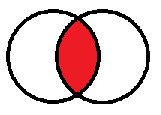
\includegraphics[width=3cm]{6_1_1}
\center{$A \wedge B$}
\end{minipage}
\begin{minipage}[c]{3.5cm}

\includegraphics[width=3cm]{6_1_2}
\center{$A \vee B$}
\end{minipage}
\begin{minipage}[r]{3.5cm}

\includegraphics[width=3cm]{6_1_3}
\center{$A \oplus B$}
\end{minipage}
\\
\\
$A \oplus B = (\neg(A\wedge B))\wedge(A\vee B) = \neg((A\wedge B)\vee(\neg A\wedge \neg B))$
\\
\begin{center}
\textbf{������� ���������� ��� $A \oplus B$}
\end{center}
\begin{minipage}[l]{4cm}
\begin{tabular}{|c|c|c|}
\hline
A & B & A $\oplus$ B \\
\hline
0 & 0 & 0 \\
0 & 1 & 1 \\
1 & 0 & 1 \\
1 & 1 & 0 \\
\hline
\end{tabular}
\end{minipage}
\begin{minipage}[l]{6cm}
\begin{tabular}{|c|c|c|c|}
\hline
A & B & C & A $\oplus$ B $\oplus$ C\\
\hline
0 & 0 & 0 & 0 \\
0 & 0 & 1 & 1 \\
0 & 1 & 0 & 1 \\
0 & 1 & 1 & 0 \\
1 & 0 & 0 & 1 \\
1 & 0 & 1 & 0 \\
1 & 1 & 0 & 0 \\
1 & 1 & 1 & 1 \\
\hline
\end{tabular}
\end{minipage}
\\
\\� ������ ���� ���������� ��������� ���������� �������� �������� �������� ����� � ������ �����, ����� ���� ���� �� ���������� �������� ��������.
\\��� ������� ���� � ����� ���������� ��������� ���������� �������� ����� �������� ������ �����, ����� ���������� ����������, ������ 1, - ��������.
\begin{center}
  \textbf{������ ����������� ������}
\end{center}
��������, � ��� ���� ���� �������������� ��� $i = 1$. � ���� ���� ���� $r_1$ - ��� ��������, ����������� ������ �1.
\\$i = r_1$, $i \oplus r_1 = 0$.
\\��� ��������� ������ ��������� ���� � ������ �����������. ��� ��������, ��� ����� �� ������ 2 ��������������� ���� � ���� �������� ����� 0.
\begin{table}[h]
\begin{tabular}{|c|c|c|c|c|}
\hline
i ��� & $r_{1}$ ��� & i ��� & $r_{1}$ ��� & i ��� $\oplus$ $r_{1}$ ��� \\
\hline
1 & 1 & 0 & 0 & 0 \\
1 & 1 & 0 & 1 & 1 \\
1 & 1 & 1 & 0 & 1 \\
1 & 1 & 1 & 1 & 0 \\
\hline
\end{tabular}
\end{table}
\\��������������, ���� � �������� "���"\ - ��������, � "���"\ - ��������������.
\\� ������ ������ �����, ��� �������� �� ��, ��� ��� ���� ������ � �������, ����� �� ������ 2 ����� ���� (�����), � ������ ��������� �� ��������� ��� ��� �� ������.
\\�� ������ � ������� ������� ����� �� ������ 2 �������������� ������ �� �����, ����� 1. ������.
\\� ��������� ������ ��� �����. ���� ���������, ����� �� ������ 2 �����. ������ ���.
\\
\\������ ����������� ������ � ������� ���� �������� ����������� � RAID-���������� (RAID - (����. redundant array of independent disks - ���������� ������ ����������� ������) ���������� ������������� ������, ������� ���������� ��������� ������ � ���������� ������� ��� ������������ � ��������� ������������������).

\section{��� ��������}
\begin{wrapfigure}[14]{l}{2.8cm}
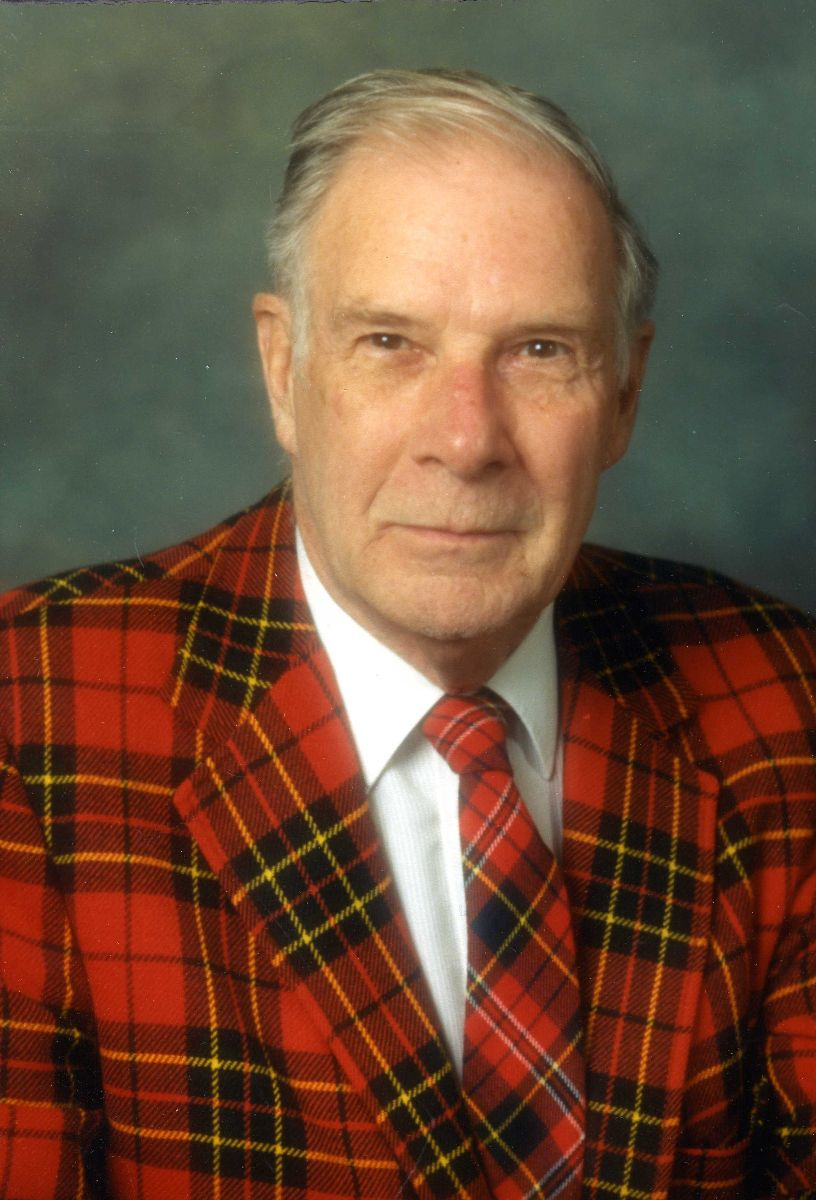
\includegraphics[width=2.8cm]{6_2_1}
\begin{center}
\footnotesize{������ ����� �������}
\\\footnotesize{$1915 - 1998$}
\end{center}
\end{wrapfigure}
� 1945 ���� ������� ��������� ���������������� ������ �� ������ ����������� �������� ����������� ��� ������� ������� ���������� ���������.  � ������ � 1946 �� 1976 ���� ������� ������� � Bell Labs, ��� ����������� � ������ ��������. ������� ����� ������� � �������� ���, � ��� ������ � ������ �����������, ������ ��� ����� ��� ������ ������������� ���� ��������� ��-�� ������������ ���������. �� ���������� ���������� ��� �� �������� ����� ������� ��� ����������� ����������� ���������� ����������� ������. � 1950 ���� �� ����������� ������, ������� �� ����������� ���� �������� ��� \textbf{\emph{��� ��������}}. ���� �������� � �������� ��������� �, ��������, ������ �� \emph{��������������������} � \emph{��������������������} �����.\\
���������� ��������� ��� ���� ���� �����:
\begin{itemize}
\item \emph{�������������������� ����} -- ����, ����������� ������������� ������������ ������ ��� �������� ������. ��� �� ���������� ���������� ��������� � ������� ����� ���� ���������� (�����������) �������� ������ � ������� ����� ����� ������� ���, ����� ����� ���������� ������ � ����������� ������ ����� ����, ��������, ������. ��������� ������ � �����-���� ������� ������������� ����� (� ��� �����, ����� ����, � � ����������� �������) ������� �������� ������ ���������� ������. �������� �� ������ 2, �������������� ���������� ������, ������� ���������� ����� �������� ���� �����, ����� ������ ������ � ������� ������.\\
\\��� ���� ���������� ������, � ����� ������ ������� ��������� ������, �, �������������, ��� ����������� ��������� �. �������� ������������� ����� ������, ����������� ������������ � ����, � ������ ��� ������ � ������ ���������� ��������. �������, �������, � ��� ����� ������������� ������ ���������� ��������������.
\item \emph{�������������������� ����} -- ����, � ������� �������� �������������� ����������� ������. ��� ���������� ��������������������� ����, ������������� �� ����������� ��������� ������, ������ ������������ ������� ������������. ��� ����� �� �����������, ���������� ����������� �������� k ������ ���� ������� ���, ����� ��������������� ����������� $2^k \ge k+m+1$ ��� $k \ge log_2{k+m+1}$, ��� m -  ���������� �������� �������� �������� �������� �����. ����������� �������� k ��� �������� ��������� m, ��������� � ������������ � ���� ������������, ��������� � �������.

\begin{table}[h]
\begin{center}
\begin{tabular}{|c|c|}
\hline
 �������� m & $k_{min}$  \\
\hline
1 & 2 \\
\hline
2-4 & 3\\
\hline
5-11 & 4\\
\hline
12-26 & 5\\
\hline
27-57 & 6 \\
\hline
\end{tabular}
\end{center}
\end{table}
\end{itemize}
� ��������� ����� ���������� ������� ������������ �������� ������� �������������� ����. ��� ������������� ����� ����� ���������� ��������� � ���� ������ ���������� ����� � ������ ���� ���������� � ������������ ���������� ���� �� �����. ����� �� ���� ������� ����� ������� ����� ��������� �� �������������� � �����������. ����� �������, ��� ���������� ����� ����������� �� ����������� (��� ������� ����������� �������������� � ����������� �������� ��������) � �����������.\\
\\\textbf{��� ��������} - ������� ����������� ���������� �������������������� ���. ���������� ��������� ������� ������, ��������� ��� �������� ��� �������� ������.
\\
\\�� ������ $i$ �������������� ��� ������������ $r$ �����������.
\\
\\�������� ������� ������������ ���� ������� �� �������� �������������� ���: ����������� ��� � ������� $N$ ������������ ��� ����������� $N$ ��� ����� ������ $N$ ���, ������� � ������� $N$.
\\\textbf{������� ������������������ S} - ����� ����������� ���� �������������� � ����������� ��������
\\
\\���������� �������:
\begin{table}[h]
\begin{tabular}{|c|c|c|c|c|c|c|c|c|c|c|c|c|c|c|c|}
\hline
& 1 & 2 & 3 & 4 & 5 & 6 & 7 & 8 & 9 & 10 & 11 & 12 & 13 & 14 & \\
\hline
$2^k$ & $r_{1}$ & $r_{2}$ & $i_{1}$ & $r_{3}$ & $i_{2}$ & $i_{3}$ & $i_{4}$ & $r_{4}$ & $i_{5}$ & $i_{6}$ & $i_{7}$ & $i_{8}$ & $i_{9}$ & $i_{10}$ & S\\
\hline
1 & \cellcolor{Gray1}{X} & & \cellcolor{Gray1}{X} & & \cellcolor{Gray1}{X} & & \cellcolor{Gray1}{X} & & \cellcolor{Gray1}{X} & & \cellcolor{Gray1}{X} & & \cellcolor{Gray1}{X} & & $s_{1}$\\
\hline
2 & & \cellcolor{Gray2}{X} & \cellcolor{Gray2}{X} & & & \cellcolor{Gray2}{X} & \cellcolor{Gray2}{X} & & & \cellcolor{Gray2}{X} & \cellcolor{Gray2}{X} & & & \cellcolor{Gray2}{X} & $s_{2}$ \\
\hline
4 & & & & \cellcolor{Gray3}{X} & \cellcolor{Gray3}{X} & \cellcolor{Gray3}{X} & \cellcolor{Gray3}{X} & & & & & \cellcolor{Gray3}{X} & \cellcolor{Gray3}{X} & \cellcolor{Gray3}{X} & $s_{3}$ \\
\hline
8 & & & & & & & & \cellcolor{Gray4}{X} & \cellcolor{Gray4}{X} & \cellcolor{Gray4}{X} & \cellcolor{Gray4}{X} & \cellcolor{Gray4}{X} & \cellcolor{Gray4}{X} & \cellcolor{Gray4}{X} & $s_{4}$ \\
\hline
\end{tabular}
\end{table}
\\������ ������� ������������ ��� ���� �� 14 ���, �� �� ����� ��������� ��� ������� ������� ��������������.
\\������ (� ������ �������) ������ ����� ����, � ������ - �������.
\\������ $X$ ���������� �� ����, ������� ������������ ����������� ���, � �������, ������� ������ � ����� ������� (������� ������). ����� ������ ������ ������ �������������� ��� � ������� $N$ ���� ������ ��������� $N$ �� �������� ������.
\\��������, �����, ��� ����������� ��� $r_1$ ������������ �������������� ���� $i_1$, $i_2$, $i_4$, $i_5$, $i_7$, $i_9$. � 11 ��� ($i_7$) �������������� ������ 1 ($r_1$), 2 ($r_2$) � 8 ($r_4$).
\\����� ������ �������� ������������ ���� ���������� ������� �� ������ 2 ��� �������������� ����, ������� �� ������������.
\\� ������ ������:
\\$r_1 = i_1\oplus i_2\oplus i_4\oplus i_5\oplus i_7\oplus i_9$;
\\$r_2 = i_1\oplus i_3\oplus i_4\oplus i_6\oplus i_7\oplus i_10$;
\\� ��� �����.
\\����� ������ �������� ��������, ���������� ������� �� ������ 2 ��� ����, ������� �������� �������.
\\� ������ ������:
\\$s_1 = r_1\oplus i_1\oplus i_2\oplus i_4\oplus i_5\oplus i_7\oplus i_9$;
\\$s_2 = r_2\oplus i_1\oplus i_3\oplus i_4\oplus i_6\oplus i_7\oplus i_{10}$;
\\� ��� �����.
\\������� ������������������ S ������������ ������������� ���������� $s_1$, $s_2$ � ��� �����. �� ���� ��� ����, ��� $r = 3$, ������� ����� ����� ��������� ������: $S(s_1;s_2;s_3)$.
\\
\\����������� ������������ ���������� ����������� ��������: $$2^k \ge r + i + 1$$.
\\������������ ���� �������� � ����������� (n, i): (7, 4); (15, 11); (31, 26).
\\
\\������� ��� �������� ��� $r = 3$.
\begin{center}
\textbf{��� �������� ��� $r = 3$}
\end{center}
� ������ ������, � ��� 7 ���, �� ��� 4 �������������� � 3 �����������. �� ����, ��� ����� ���������� (7, 4).
\\�������� ������� ���� (7, 4):
\begin{table}[h]
\begin{tabular}{|c|c|c|c|c|c|c|c|c|}
\hline
& 1 & 2 & 3 & 4 & 5 & 6 & 7 & \\
\hline
$2^k$ & $r_{1}$ & $r_{2}$ & $i_{1}$ & $r_{3}$ & $i_{2}$ & $i_{3}$ & $i_{4}$ & S\\
\hline
1 & \cellcolor{Gray1}{X} & & \cellcolor{Gray1}{X} & & \cellcolor{Gray1}{X} & & \cellcolor{Gray1}{X} & $s_{1}$\\
\hline
2 & & \cellcolor{Gray2}{X} & \cellcolor{Gray2}{X} & & & \cellcolor{Gray2}{X} & \cellcolor{Gray2}{X} & $s_{2}$ \\
\hline
4 & & & & \cellcolor{Gray3}{X} & \cellcolor{Gray3}{X} & \cellcolor{Gray3}{X} & \cellcolor{Gray3}{X} & $s_{3}$ \\
\hline
\end{tabular}
\end{table}
\\���������� ��������� �������� �������������� ��� ������������ �� ������ ������:
\\
\begin{minipage}[l]{3.5cm}
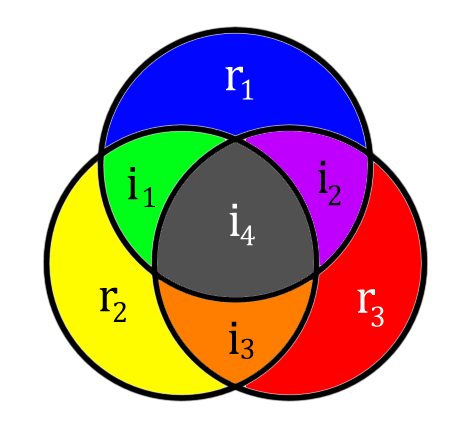
\includegraphics[width=3.5cm]{6_2_2}
\end{minipage}
\begin{minipage}[r]{9cm}
�����, ��� $r_1$ ������������ $i_1$, $i_2$ � $i_4$; $r_2$ ������������ $i_1$, $i_3$ � $i_4$; � $r_3$ ������������ $i_2$, $i_3$ � $i_4$.
\\$r_1 = i_1 \oplus i_2 \oplus i_4$
\\$r_2 = i_1 \oplus i_3 \oplus i_4$
\\$r_3 = i_2 \oplus i_3 \oplus i_4$
\end{minipage}
\\
\\$s_1 = r_1 \oplus i_1 \oplus i_2 \oplus i_4$
\\$s_2 = r_2 \oplus i_1 \oplus i_3 \oplus i_4$
\\$s_3 = r_3 \oplus i_2 \oplus i_3 \oplus i_4$
\\
\\���������� ������� �������� �������� ($s_1;s_2;s_3$) � ������� ���������� ���� � ���������:
\begin{table}[h]
\begin{tabular}{|c|c|c|}
\hline
������� ($s_1;s_2;s_3$) & ������������ ������ & ��������� ������\\
\hline
000 & ��� & ��� \\
001 & 0001000 & $r_3$ \\
010 & 0100000 & $r_2$ \\
011 & 0000010 & $i_3$ \\
100 & 1000000 & $r_1$ \\
101 & 0000100 & $i_2$ \\
110 & 0010000 & $i_1$ \\
111 & 0000001 & $i_4$ \\
\hline
\end{tabular}
\end{table}\\
�������, � �������, 2 ������ (��. ������� �� ��������� ��������) : ������� $S(0,0,1)$, ��� ������ ��� $s_1 = 0$, $s_2 = 0$, $s_3 = 1$. �� ����������� ������� ���� (7,4) ���������, � ����� ���� ������ - ����� ��� ���������� ������ � 3 ��������. ����� ������, � ����� ������� $X$ ����� ������ � 3 ������� (�������� $s_3$). �� ������� �����, ��� ����� ��� - 4 (������� �� ������ ������� 0001000 - ���� �������� ���������� ���, � ������� - ���������. � ������ ������ ��������� ��� 4, ������� �� ����� �������). �������, ����� ������ ��� �������� ��������� ����� - $r_3$.
\\����� �������� ���������� ������������������, ���������� ������������� ��������� ���.
\\
\\\emph{\textbf{������ 1:}}
\\\emph{�������:} �������� ������������������ 1100100. ��������� ��������� ���, �������� ���������� ������������������.
\\\emph{�������:} �������� ������� ���� (7,4) � ���������� �������������������.
\begin{table}[h]
\begin{tabular}{|c|c|c|c|c|c|c|c|c|}
\hline
& 1 & 2 & 3 & 4 & 5 & 6 & 7 & \\
\rowcolor{Gray1}
\hline
& 1 & 1 & 0 & 0 & 1 & 0 & 0 & \\
\hline
$2^k$ & $r_{1}$ & $r_{2}$ & $i_{1}$ & $r_{3}$ & $i_{2}$ & $i_{3}$ & $i_{4}$ & S\\
\hline
1 & \cellcolor{Gray1}{X} & & \cellcolor{Gray1}{X} & & \cellcolor{Gray1}{X} & & \cellcolor{Gray1}{X} & $s_{1}$\\
\hline
2 & & \cellcolor{Gray2}{X} & \cellcolor{Gray2}{X} & & & \cellcolor{Gray2}{X} & \cellcolor{Gray2}{X} & $s_{2}$ \\
\hline
4 & & & & \cellcolor{Gray3}{X} & \cellcolor{Gray3}{X} & \cellcolor{Gray3}{X} & \cellcolor{Gray3}{X} & $s_{3}$ \\
\hline
\end{tabular}
\end{table}
\\���������� �������� ����������� ��� ����������:
\\$r_{1\mbox{ ���}} = i_1 \oplus i_2 \oplus i_4 = 0 \oplus 1 \oplus 0 = 1$
\\$r_{2\mbox{ ���}} = i_1 \oplus i_3 \oplus i_4 = 0 \oplus 0 \oplus 0 = 0$
\\$r_{3\mbox{ ���}} = i_2 \oplus i_3 \oplus i_4 = 1 \oplus 0 \oplus 0 = 1$
\\���������� ��������:
\\$s_1 = r_1 \oplus i_1 \oplus i_2 \oplus i_4 = r_{1\mbox{ ���}} \oplus r_{1\mbox{ ���}} = 1 \oplus 1 = 0$
\\$s_2 = r_2 \oplus i_1 \oplus i_3 \oplus i_4 = r_{2\mbox{ ���}} \oplus r_{2\mbox{ ���}} = 0 \oplus 1 = 1$
\\$s_3 = r_3 \oplus i_2 \oplus i_3 \oplus i_4 = r_{3\mbox{ ���}} \oplus r_{3\mbox{ ���}} = 1 \oplus 0 = 1$
\\���������� �������: $S(0,1,1)$.
\\������� �� �������, ����� ��� ���������� � $s_2$ � $s_3$ ������������. 6, �� ���� $i_3$.
\\����������� ��������� ��� � �������� ���������� ������������������.
\\�����: 6 ��� ($i_3$), ���������� ������������������: 1100110.
\begin{figure}
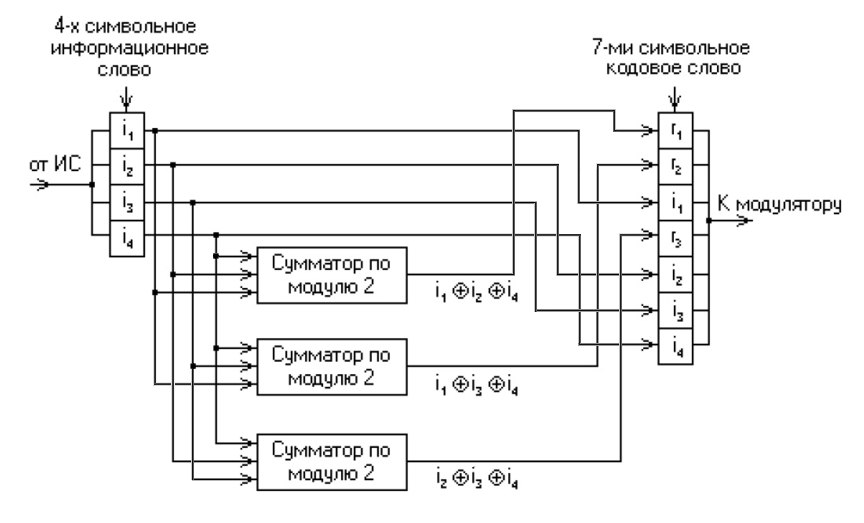
\includegraphics[width=\textwidth]{6_2_3}
\caption{����� �������� ���� �������� (7,4)}
\end{figure}
\begin{figure}
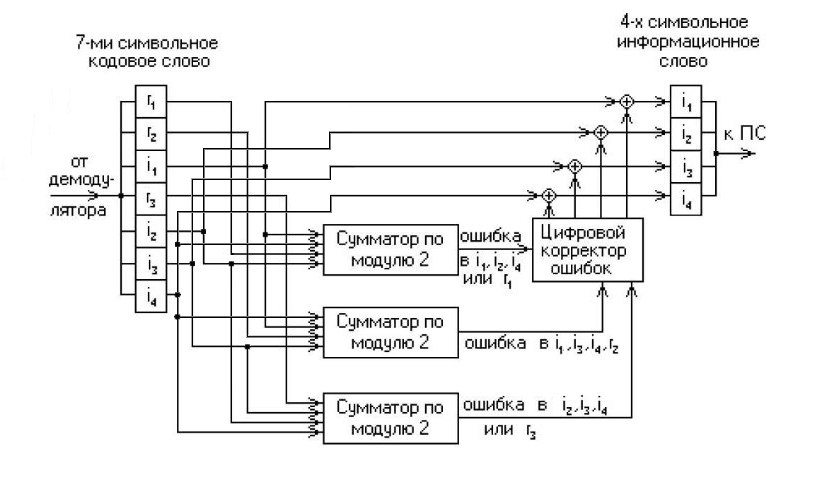
\includegraphics[width=\textwidth]{6_2_4}
\caption{����� ������������� ���� �������� (7,4)}
\end{figure}
\newpage
������� ��� �������� ��� $r = 4$ ���������� ����, ��� �� ������� ��� ����.
\begin{center}
\textbf{��� �������� ��� $r = 4$}
\end{center}
� ������ ������, � ��� 15 ���, �� ��� 11 �������������� � 4 �����������. �� ����, ��� ����� ���������� (15, 11).
\\�������� ������� ���� (15, 11):
\begin{table}[h]
\begin{tabular}{|c|c|c|c|c|c|c|c|c|c|c|c|c|c|c|c|c|}
\hline
& 1 & 2 & 3 & 4 & 5 & 6 & 7 & 8 & 9 & 10 & 11 & 12 & 13 & 14 & 15 & \\
\hline
$2^k$ & $r_{1}$ & $r_{2}$ & $i_{1}$ & $r_{3}$ & $i_{2}$ & $i_{3}$ & $i_{4}$ & $r_{4}$ & $i_{5}$ & $i_{6}$ & $i_{7}$ & $i_{8}$ & $i_{9}$ & $i_{10}$& $i_{11}$ &S\\
\hline
1 & \cellcolor{Gray1}{X} & & \cellcolor{Gray1}{X} & & \cellcolor{Gray1}{X} & & \cellcolor{Gray1}{X} & & \cellcolor{Gray1}{X} & & \cellcolor{Gray1}{X} & & \cellcolor{Gray1}{X} & & \cellcolor{Gray1}{X} & $s_{1}$\\
\hline
2 & & \cellcolor{Gray2}{X} & \cellcolor{Gray2}{X} & & & \cellcolor{Gray2}{X} & \cellcolor{Gray2}{X} & & & \cellcolor{Gray2}{X} & \cellcolor{Gray2}{X} & & & \cellcolor{Gray2}{X} & \cellcolor{Gray2}{X} & $s_{2}$ \\
\hline
4 & & & & \cellcolor{Gray3}{X} & \cellcolor{Gray3}{X} & \cellcolor{Gray3}{X} & \cellcolor{Gray3}{X} & & & & & \cellcolor{Gray3}{X} & \cellcolor{Gray3}{X} & \cellcolor{Gray3}{X} & \cellcolor{Gray3}{X} & $s_{3}$ \\
\hline
8 & & & & & & & & \cellcolor{Gray4}{X} & \cellcolor{Gray4}{X} & \cellcolor{Gray4}{X} & \cellcolor{Gray4}{X} & \cellcolor{Gray4}{X} & \cellcolor{Gray4}{X} & \cellcolor{Gray4}{X} & \cellcolor{Gray4}{X} & $s_{4}$\\
\hline
\end{tabular}
\end{table}
�������: 
\\$r_1 = i_1 \oplus i_2 \oplus i_4  \oplus i_5  \oplus i_7  \oplus i_9  \oplus i_{11}$ 
\\$r_2 = i_1 \oplus i_3 \oplus i_4  \oplus i_6  \oplus i_7  \oplus i_{10}  \oplus i_{11}$
\\$r_3 = i_2 \oplus i_3 \oplus i_4  \oplus i_8  \oplus i_9  \oplus i_{10}  \oplus i_{11}$
\\$r_4 = i_5 \oplus i_6 \oplus i_7  \oplus i_8  \oplus i_9  \oplus i_{10}  \oplus i_{11}$
\\
\\$s_1 = r_1 \oplus i_1 \oplus i_2 \oplus i_4  \oplus i_5  \oplus i_7  \oplus i_9  \oplus i_{11}$
\\$s_2 = r_2 \oplus i_1 \oplus i_3 \oplus i_4 \oplus i_6  \oplus i_7  \oplus i_{10}  \oplus i_{11}$
\\$s_3 = r_3 \oplus i_2 \oplus i_3 \oplus i_4 \oplus i_8  \oplus i_9  \oplus i_{10}  \oplus i_{11}$
\\$s_4 = r_4 \oplus i_5 \oplus i_6 \oplus i_7  \oplus i_8  \oplus i_9  \oplus i_{10}  \oplus i_{11}$
\\
\\���������� ������� �������� �������� ($s_1;s_2;s_3;s_4$) � ������� ���������� ���� � ���������: \\\\
����������� ����� ����������. �������, ��������, 4�� ������ (��. ������� �� ��������� ��������). ������� S(0,0,1,1) ��������, ��� $s_1 = 0$, $s_2 = 0$, $s_3 = 1$, $s_4 = 1$. �� ������� ���� (15,11) ���������, � ����� ���� ������ - ����� ��� ���������� ������ � 4 ��������. � ������ ������, ����� ��� - 12. ��������, ��� ���� ���������� ���������� ���, � ������� - ���������. ����������� ����� �������� ��� $i_8$.
\begin{tabular}{|c|c|c|c|}
\hline
������� ($s_1;s_2;s_3;s_4$) & ������������ ������ & ��������� ������\\
\hline
0000 & ��� & ��� \\
0001 & 000000010000000 & $r_4$ \\
0010 & 000100000000000 & $r_3$ \\
0011 & 000000000001000 & $i_8$ \\
0100 & 010000000000000 & $r_2$ \\
0101 & 000000000100000 & $i_6$ \\
0110 & 000001000000000 & $i_3$ \\
0111 & 000000000000010 & $i_{10}$ \\
1000 & 100000000000000 & $r_1$\\
1001 & 000000001000000 & $i_5$\\
1010 & 000010000000000& $i_2$\\
1011 & 000000000000100 & $i_9$\\
1100 & 001000000000000 & $i_1$\\
1101 & 000000000010000 & $i_7$\\
1110 & 000000100000000 & $i_4$\\
1111 & 000000000000001 & $i_{11}$\\
\hline
\end{tabular}

\chapter{Алгебра логики}
Как было рассмотрено ранее, информатика изучает знаковые(алфавитные) системы. \textbf{Алгебра} -- наиболее адекватный математический аппарат описания действий в них, поэтому алгебраический аппарат наилучшим образом подходит для описания информационных систем общей природы, отвлеченно от их предметной направленности. Информационные процессы хорошо формализуются с помощью различных алгебраических структур. \\
\\Кроме обычной алгебры существует специальная, основы которой были заложены английским математиком XIX века Дж. Булем. Эта алгебра занимается так называемым исчислением высказываний.Ее особенностью является применимость для описания работы так называемых дискретных устройств, к числу которых принадлежит целый класс устройств автоматики и вычислительной техники.
\section{Определение}
\begin{wrapfigure}[13]{l}{2.8cm}
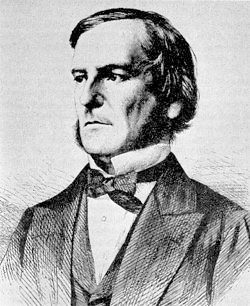
\includegraphics[width=2.8cm]{7_1}
\begin{center}
\footnotesize{Джордж Буль}
\\\footnotesize{$1815 - 1864$}
\end{center}
\end{wrapfigure}
\textbf{Алгебра двоичной логики} -- раздел математики, в котором изучаются логические операции над высказываниями. Чаще всего предполагается, что высказывания могут быть только истинными или ложными, то есть используется так называемая бинарная или двоичная логика. Один из основателей алгебры логики - Джордж Буль.
\\
\\\textbf{Логическая (булева) переменная} – такая переменная, значения которой могут быть лишь "1" или "0".
\\\emph{В естественном языке:} "булева переменная" $=$ "высказывание".
\\
\textbf{\\Высказывание} -- утверждение, про которое можно однозначно сказать, истинно оно или ложно.
\\\emph{Обозначения:}
\begin{itemize}
  \item "истина" \ и "ложь"
  \item "true" \ и "false"
  \item "1" \ и "0"
\end{itemize}
Например, высказывание "Москва - столица России\"  -- истина, а "трава синего цвета\"  -- ложь.
\\
\textbf{Логическая (булева) функция $f(x, y, z, …)$} -- некоторая функциональная зависимость, в результате выполнения логических операций над логическими переменными $x, y, z,\dots$ получает значение 0 или 1.
\textbf{Таблица истинности} -- таблица всех значений некоторой \emph{логической функции}.
\begin{center}
  \emph{Основные операции}
\end{center}
$\bar{x}$ - отрицание или инверсия
\\$x \vee y$ - дизъюнкция или логическое сложение
\\$x \wedge y$ - конъюнкция или логическое умножение\\
\\Кроме указанных трех базовых операций можно с их помощью ввести еще следующие важные операции алгебры предикатов (можно их назвать небазовыми операциями):\\
$(x\to y) \equiv (\bar{x} \vee y)$ - импликация \\
$(x\leftrightarrow y) \equiv (x \wedge y \vee \bar{x} \wedge \bar{y})$ - эквиваленция\\
\\Операции импликации и эквиваленции хотя и часто используются, но не являются базовыми, ибо они определяемы через три введенные выше базовые операции. При выполнении логических операций в компьютере они сводятся к поразрядному сравнению битовых комбинаций. Эти операции достаточно быстро (аппаратно) выполняемы, так как сводятся к выяснению совпадения или несовпадения битов.\\
\\В логических формулах определено старшинство операций, например: скобки, отрицание, конъюнкция, дизъюнкция (остальные, небазовые операции пока не учитываем).\\
\\Всегда истинные формулы называют \textbf{тавтологиями}.\\
\\\emph{Логические функции} эквивалентны, если совпадают их таблицы истинности, то есть совпадают области определения и значения, а также сами значения функции при одних и тех же наборах переменных из числа всех допустимых значений. Если это совпадение происходит на части множества допустимых значений, то формулы называются эквивалентными лишь на этой части (на этом подмножестве).\\
\\Задача \textbf{упрощения логического выражения} состоит в преобразовании его к более простому (по числу переменных, операций или операндов) эквивалентному выражению. Наиболее простой вид получается при сведении функции к постоянной – 1 (истина) или 0 (ложь).


\section{Основные тождества}
\begin{enumerate}
  \item Аксиома двойного отрицания \\
     $$\bar{\bar{x}} = x$$
  \item Аксиома существования 1 и 0 \\
  \begin{minipage}{5cm}
     $$0 = \bar{1}$$
     $$1 = \bar{0}$$
  \end{minipage}
  \begin{minipage}{5cm}
     $$x \vee \bar{x} = 1$$
     $$x \wedge \bar{x} = 0$$
  \end{minipage}
  \item Закон идемпотенции \\
  \begin{minipage}{5cm}
     $$x \vee x = x$$
  \end{minipage}
  \begin{minipage}{5cm}
     $$x \wedge x = x$$
  \end{minipage}
  \item Закон коммутативности \\
  \begin{minipage}{5cm}
     $$x \vee y = y \vee x$$
  \end{minipage}
  \begin{minipage}{5cm}
     $$x \wedge y = y \wedge x$$
  \end{minipage}
  \item Закон поглощения \\
  \begin{minipage}{5cm}
     $$x \vee (x \wedge y) = x$$
  \end{minipage}
  \begin{minipage}{5cm}
     $$x \wedge (x \vee y) = x$$
  \end{minipage}
  \item Закон ассоциативности \\
  \begin{minipage}{5cm}
     $$x \vee (y \vee z) = (x \vee y) \vee z$$
  \end{minipage}
  \begin{minipage}{5cm}
     $$x \wedge (y \wedge z) = (x \wedge y) \wedge z$$
  \end{minipage}
  \item Закон дистрибутивности \\
  \begin{minipage}{5cm}
     $$x \vee (y \wedge z) = (x \vee y) \wedge (x \vee z)$$
  \end{minipage}
  \begin{minipage}{5cm}
     $$x \wedge (y \vee z) = (x \wedge y) \vee (x \wedge z)$$
  \end{minipage}
  \item Законы де Моргана \\
  \begin{minipage}{5cm}
     $$\bar{x \vee y} = \bar{x} \wedge \bar{y}$$
  \end{minipage}
  \begin{minipage}{5cm}
     $$\bar{x \wedge y} = \bar{x} \vee \bar{y}$$
  \end{minipage}
  \item Закон нейтральности \\
  \begin{minipage}{5cm}
     $$x \vee (y \wedge \bar{y}) = x$$
  \end{minipage}
  \begin{minipage}{5cm}
     $$x \wedge (y \vee \bar{y}) = x$$
  \end{minipage}
\end{enumerate}

\section{Таблица истинности}
Существует только 4 различные логические функции одной переменной $F(x)$. Любая другая функция (даже самая сложная вида $F(x) = \bar{x} \vee x \wedge \bar{x}$) будет иметь одну из следующих таблиц истинности:
\begin{table}[!h]
\begin{tabular}{|c||c|c|c|c|}
\hline
$x$ & $F_0(x)$ & $F_1(x)$ & $F_2(x)$ & $F_3(x)$ \\
\hline
\hline
0 & 0 & 1 & 0 & 1 \\
\hline
1 & 0 & 0 & 1 & 1 \\
\hline
\end{tabular}
\end{table}
\\Например $F(x) = \bar{x}$ будет иметь таблицу истинности $F_1(x)$, а $F(x) = 1$ - $F_3(x)$
\\
\\Обычно логическую функцию $F(x)$ обозначают как $FK,N$, где $K$ - количество операндов, а $N$ - число в десятичной системе счисления, которое при переводе в двоичную является таблицей истинности функции. Например, $F(x) = \bar{x}$ обозначается как $F1,2$, так как одна переменная и $2_{10} = 01_{2}$, что является таблицей истинности функции (смотреть снизу вверх).
\\
\\Для $k$ переменных будет существовать $N = 2^{2^{k}}$ функций.
\\Рассмотрим таблицу истинности:
\\
\\
\begin{minipage}{2cm}
\begin{center}
$L$ штук\\
(от 00..0\\ до 11..1 \\ сверху \\ вниз)
\end{center}
\end{minipage}
\begin{minipage}{0.3cm}
\quad \\
\quad \\
$\left\{
\begin{array}{c}
\\
\\
\\
\\
\end{array}
\right.$
\quad \\
\end{minipage}
\begin{minipage}[l]{9cm}
\begin{tabular}{c|c|c|c|c|c|c|c|c|}
\hhline{~--------}
& \multicolumn{4}{c|}{Значения $k$ штук} & \multicolumn{4}{c|}{\multirow{2}{*}{Значение булевых функций $F$}} \\
& \multicolumn{4}{c|}{булевых операндов} & \multicolumn{4}{c|}{}\\
\hhline{~--------}
& $x_1$ & $x_2$ & \dots & $x_k$ & $FK,0$ & $FK,1$ & \dots & $FK,N$ \\
\hhline{~--------}
 & 0 & 0 & \dots & 0 & 0 & 1 & \dots & 1\\
& 0 & 0 & \dots & 1 & 0 & 0 & \dots & 1\\
& \dots & \dots & \dots & \dots & \dots & \dots & \dots & \dots\\
\multirow{4}{*}{} & 1 & 1 & \dots & 1 & 0 & 0 & \dots & 1\\

\hhline{~--------}
\multicolumn{5}{c}{} & \multicolumn{4}{c}{$\underbrace{\qquad \qquad \qquad \qquad \qquad \qquad \qquad}_{\mbox{от N штук (от 00..0 }}$} \\
\multicolumn{5}{c}{} & \multicolumn{4}{c}{до 11..1 слева направо)}
\end{tabular}
\end{minipage}
\\
\\
\\
Так как всего $k$ переменных, то для них будет $L = 2^k$ строк в таблице истинности, а количество булевых функций будет равно $N = 2^L$. Отсюда:
\\
\begin{center}
\begin{tabular}{c c}
$L = 2^k$ & \multirow{2}{*}{$\Rightarrow N = 2^{2^{k}}$} \\
$N = 2^L$ & \\
\end{tabular}
\end{center}
Так, для 1 переменной будет 4 булевых функции, для 2 переменных - 16 и так далее.
\begin{table}[!h]
\begin{tabular}{|c|c|c|c|c|c|c|}
\hline
$x$ & 1 & 1 & 0 & 0 & \multirow{2}{*}{Обозначение} & \multirow{2}{*}{Название} \\
\hhline{-----~~}
$y$ & 1 & 0 & 1 & 0 & & \\
\hline
\multirow{2}{*}{F} & \multirow{2}{*}{0} & \multirow{2}{*}{0} & \multirow{2}{*}{0} & \multirow{2}{*}{0} & F2,0 = $FALSE$  & Противоречие,  \\
& & & & & & логичечский нуль \\
\hline
\multirow{3}{*}{F} & \multirow{3}{*}{0} & \multirow{3}{*}{0} & \multirow{3}{*}{0} & \multirow{3}{*}{1} & F2,1 = $x\downarrow y = x NOR y = $  & Cтрелка Пирса, НЕ-ИЛИ, \\
& & & & & $= NOR(x,y) = x $НЕ-ИЛИ & антидизъюнкция \\
& & & & & $y = $НЕ-ИЛИ$(x,y)$ & \\
\hline
\multirow{2}{*}{F} & \multirow{2}{*}{0} & \multirow{2}{*}{0} & \multirow{2}{*}{1} & \multirow{2}{*}{0} & F2,2 = $x\leftarrow /y$  & Отрицание \\
& & & & & & обратной импликации \\
\hline
\multirow{1}{*}{F} & \multirow{1}{*}{0} & \multirow{1}{*}{0} & \multirow{1}{*}{1} & \multirow{1}{*}{1} & F2,3 = $\neg x $  &  Отрицание\\
\hline
\multirow{3}{*}{F} & \multirow{3}{*}{0} & \multirow{3}{*}{1} & \multirow{3}{*}{0} & \multirow{3}{*}{0} & F2,4 = $x\rightarrow /y $  & Материальная \\
& & & & & & обратная импликация \\
\hline
\multirow{1}{*}{F} & \multirow{1}{*}{0} & \multirow{1}{*}{1} & \multirow{1}{*}{0} & \multirow{1}{*}{1} & F2,5 = $ \neg y$  & Отрицание \\
\hline
\multirow{4}{*}{F} & \multirow{4}{*}{0} & \multirow{4}{*}{1} & \multirow{4}{*}{1} & \multirow{4}{*}{0} & F2,6 =  $x \oplus y$ = & Сложение по модулю 2, \\
& & & & & = $x XOR y = XOR(x,y)$ = & исключающее "или" \\
& & & & & = $x >< y = x <> y$ = & сумма Жегалкина, \\
& & & & & = $x NE y = NE(x,y)$ & не равно \\
\hline
& & & & & F2,7  = x | y = & Штрих Шеффера, \\
F & 0 & 1 & 1 & 1 & = $NAND(x,y)$ = $x NAND$ & НЕ-И, 2И-НЕ, \\
& & & & & $y$ = $x$ НЕ-И $y$ = НЕ-И$(x,y)$ & антиконъюнкция\\
\hline
& & & & & F2,8 = $x \wedge y = x \cdot y =$ &  \\
\multirow{2}{*}{F} & \multirow{2}{*}{1} & \multirow{2}{*}{0} & \multirow{2}{*}{0} & \multirow{2}{*}{0} &  = $xy = x \& y = x AND y$ = & Конъюнкция,\\
& & & & & = $AND(x,y) = x $И$ y =$ & 2И, минимум \\
& & & & & = И$(x,y) = min(x,y)$	& \\
\hline
& & & & & F2,9 = $(x \equiv y) = x ~ y $= & Эквивалентность \\
F & 1 & 0 & 0 & 1 & = $x \leftrightarrow y = x EQV y = $ & равенство\\
& & & & & = $EQV(x,y)$ & \\
\hline
\multirow{1}{*}{F} & \multirow{1}{*}{1} & \multirow{1}{*}{0} & \multirow{1}{*}{1} & \multirow{1}{*}{0} & F2,10 = $y $  & Проекция, повторение\\
\hline
\multirow{2}{*}{F} & \multirow{2}{*}{1} & \multirow{2}{*}{0} & \multirow{2}{*}{1} & \multirow{2}{*}{1} & F2,11 = $x \to y = x  \supset y$ = & Импликация \\
& & & & &  = $x \le y = x LE y = LE(x,y)$ & следование  \\
\hline
\multirow{1}{*}{F} & \multirow{1}{*}{1} & \multirow{1}{*}{1} & \multirow{1}{*}{0} & \multirow{1}{*}{0} & F2,12 = $x $  & Проекция, повторение\\
\hline
\multirow{1}{*}{F} & \multirow{1}{*}{1} & \multirow{1}{*}{1} & \multirow{1}{*}{0} & \multirow{1}{*}{1} & F2,13 = $x \leftarrow y $  & Обратная импликация\\
\hline
& & & & & F2,14 = $x \vee y = x + y =$ &  \\
\multirow{2}{*}{F} & \multirow{2}{*}{1} & \multirow{2}{*}{1} & \multirow{2}{*}{1} & \multirow{2}{*}{0} & =$ x OR y = OR(x,y) = $ & Дизъюнкция,\\
& & & & & = $x$ ИЛИ $y$ = ИЛИ$(x,y)$ = & 2ИЛИ, максимум \\
& & & & & $ = max(x,y)$	& \\
\hline
\multirow{1}{*}{F} & \multirow{1}{*}{1} & \multirow{1}{*}{1} & \multirow{1}{*}{1} & \multirow{1}{*}{1} & F2,15 = $TRUE $  & Тавтология\\
\hline
\end{tabular}
\caption{Таблица значений и названий булевых функций от двух переменных}
\end{table}
\section{Обозначение на электрической схеме булевых функций}
Для аппаратной реализации булевых функций и их корректного обозначения на электрической схеме принято использовать логические элементы.
\\
\\\textbf{Логический элемент} – это простейшее устройство ЭВМ, выполняющее одну определенную логическую операцию над входными сигналами согласно правилам алгебры логики. То есть, одну из функций, рассмотренных ранее.
\begin{center}
  \textbf{Современные стандарты для условных графических обозначений (УГО) логических элементов}
\end{center}
\begin{itemize}
  \item ANSI (англ.\emph{American national standards institute} - американский национальный институт стандартов).
  \item MIL/IEC (англ.\emph{MILitary} – военный, {International Electrotechnical Commission} - международная электротехническая комиссия).
  \item DIN (нем. \emph{Deutsches Institut f{\"u}r Normung e. V.} — немецкий институт по стандартизации).
  \item ГОСТ 2.743-91, Единая система конструкторской документации. Обозначения условные графические в схемах. Элементы цифровой техники. 
\end{itemize}
\begin{table}[!h]
\centering
\begin{tabular}{|c|c|c|c|}
\hline
Название & IEC & ANSI \\
\hline
\multirow{3}{*}{НЕ, $\bar{A}$ (Инвертор)} & \multirow{3}{*}{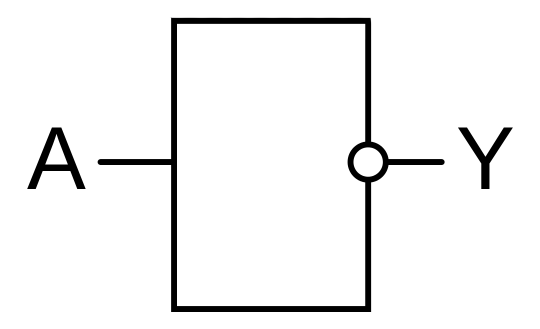
\includegraphics[width=2cm]{7_2(1)}} & \multirow{3}{*}{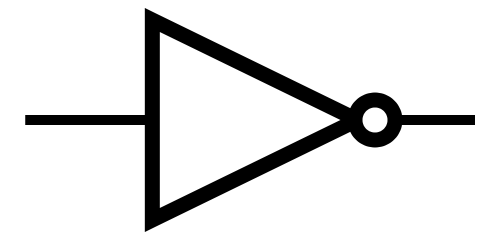
\includegraphics[width=2cm]{7_2(2)}} \\
& & \\
& & \\
\hline
\multirow{3}{*}{И, $A \wedge B$} & \multirow{3}{*}{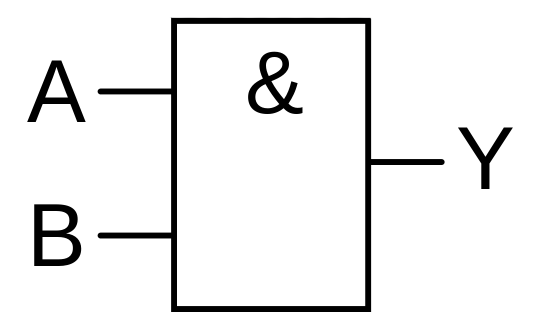
\includegraphics[width=2cm]{7_3(1)}} & \multirow{3}{*}{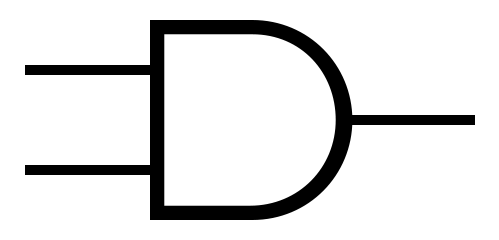
\includegraphics[width=2cm]{7_3(2)}} \\
& & \\
& & \\
\hline
\multirow{3}{*}{ИЛИ, $A \vee B$} & \multirow{3}{*}{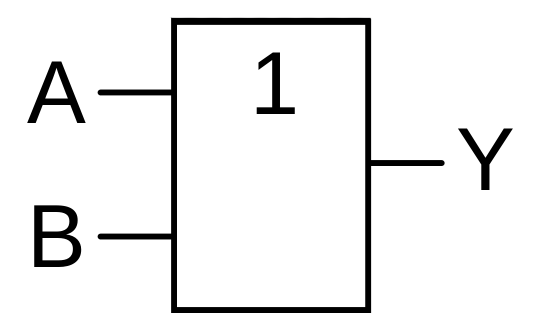
\includegraphics[width=2cm]{7_5(1)}} & \multirow{3}{*}{
\includegraphics[width=2cm]{7_5(2)}} \\
& & \\
& & \\
\hline
\multirow{3}{*}{Сумма по модулю 2, $A \oplus B$} & \multirow{3}{*}{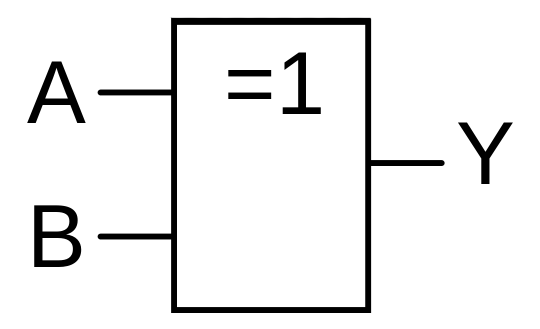
\includegraphics[width=2cm]{7_4(1)}} & \multirow{3}{*}{
\includegraphics[width=2cm]{7_4(2)}} \\
& & \\
& & \\
\hline
\end{tabular}
\caption{Обозначение некоторых булевых функций на эл. схеме}
\end{table}
%\begin{minipage}{\textwidth}
Это основные обозначения. Они могут совмещаться. Например, так будет выглядеть И-НЕ:
\\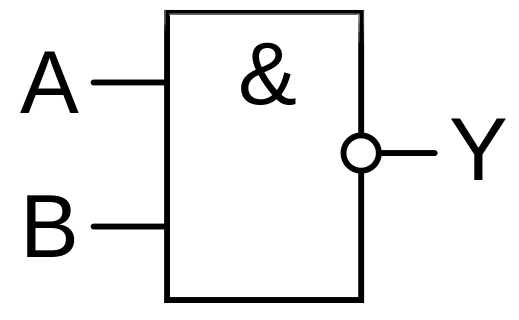
\includegraphics[width=2cm]{7_6}
%\end{minipage}
\\
\\\textbf{Цена функции по Квайну} – суммарное число входов логических элементов в составе схемы.
\\\textbf{Минимизация функции} – сокращение цены функции, с помощью преобразования её к более простому эквивалентному выражению.
Наиболее простой вид получается при сведении функции к постоянной - 1 (истина) или 0 (ложь).
\section{Логический базис}
\textbf{Логический базис} - набор булевых функций, позволяющий реализовать любую другую булеву функцию.
\\Три наиболее востребованных логических базиса: И, ИЛИ, НЕ; ИЛИ-НЕ; И-НЕ.
\begin{figure}[!h]
\centering
\caption{Пример реализации функций И, ИЛИ, НЕ в базисе И-НЕ}
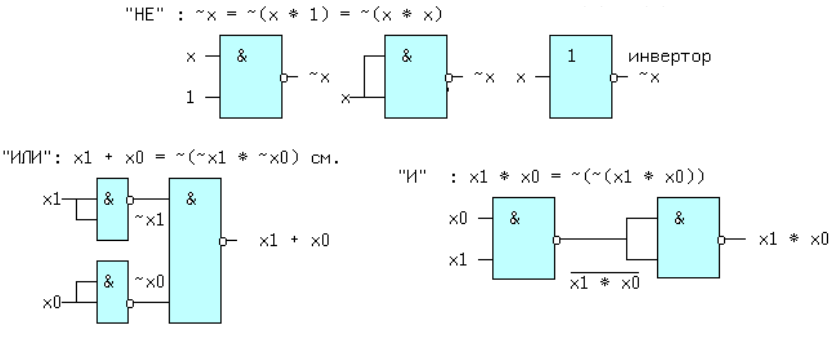
\includegraphics[width=\textwidth]{7_7}
\end{figure}
\section{Формы записи математических выражений}
Форма записи по-другому называется нотацией.
\\"Арность операции" означает количество операндов, участвующих в операции.
\\Например: $\sqrt{A}$ (унарная), $A\times B$ (бинарная).
\\
\begin{center}
 \textbf{Виды нотаций}
\end{center}
\begin{description}
  \item[1489 г.] - инфиксная запись $A + B$
  \item[1920 г.] - префиксная (польская) запись $+AB$
  \item[1957 г.] - постфиксная (обратная польская) запись $AB+$
\end{description}
\textbf{Стек} - абстрактный тип данных, представляющий собой список элементов, организованных по принципу LIFO (англ. \emph{last in - first out}, "последним пришел - первым вышел"). Чаще всего принцип работы стека сравнивают со стопкой тарелок: чтобы взять вторую сверху, нужно снять верхнюю.
\subsection{Префиксная нотация}
\textbf{\emph{Пример:}}
\\Инфиксная нотация: $(A + B + C) - E^{D\times F\times G}$
\\Префиксная нотация: $-++ABC^{\wedge}E\times\times DFG$
\\
\\Рассмотрим, как же происходит запись в префиксной нотации:
\begin{enumerate}
 \item Исходное выражение: $(A + B + C) - E^{D\times F\times G}$. Расставляем порядок выполнения операций, согласно математическим правилам.
\item Последним выполняется вычитание, а именно из $(A + B + C)$ вычитается $E^{D\times F\times G}$. \textbf{Ставим знак в начало.} Получается $-(A + B + C)(E^{D\times F\times G})$.
\item Рассмотрим $(A + B + C)$, расставим порядок действий. Сначала происходит сложение $A$ и $B$, а потом $A+B$ и $C$. Начнем с последнего действия, получается: $+(A+B)C$. В $(A+B)$ происходит сложение $A$ и $B$, получаем $(+AB)$. Совместим все вместе: $(+(+AB)C)$.
\item Рассмотрим $(E^{D\times F\times G})$, происходит возведение в степень. А именно $E$ возводится в степень $D\times F\times G$. Получается $^{\wedge}E(D\times F\times G)$.
\item Рассмотрим $D\times F\times G$, расставляем порядок действий. Сначала происходит умножение $D$ и $F$, а потом $D\times F$ и $G$. Начнем с последнего действия, получается: $\times(D \times F)G$. В $(D \times F)$ происходит умножение $D$ и $F$, получаем $(\times DF)$. Совместим все вместе: $(\times(\times DF)G)$.
\item Совмещаем все вместе. Получается: $-(+(+AB)C)(^{\wedge}E(\times(\times DF)G)$. Убираем скобки. Получили $-++ABC^{\wedge}E\times\times DFG$.
\end{enumerate}
Существует популярная Lisp-разновидность префиксной нотации (Lisp - семейство языков программирования). И в ней запись будет выглядеть так: $(-(+ABC)(^{\wedge}E(\times DFG)))$
\begin{center}
  \textbf{Особенности префиксной нотации}
\end{center}
\begin{itemize}
  \item Не требуется скобок, если арность фиксирована.
  \item Запись выражения получается короче, чем инфиксная.
  \item Не требуется знать приоритет операций.
  \item Легко декодировать выражение с помощью стека.
  \item Малоприменима на практике (кроме Lisp).
\end{itemize}
\subsection{Постфиксная нотация}
\textbf{\emph{Пример:}}
\\Инфиксная нотация: $(A + B + C) - E^{D\times F\times G}$
\\Постфиксная нотация: $CAB++EGDF\times\times ^{\wedge}-$
\\
\\Рассмотрим, как же происходит запись в постфиксной нотации:
\begin{enumerate}
\item Исходное выражение: $(A + B + C) - E^{D\times F\times G}$. Расставляем порядок выполнения операций, согласно математическим правилам.
\item Последним выполняется вычитание, а именно из $(A + B + C)$ вычитается $E^{D\times F\times G}$. \textbf{Ставим знак в конец.} Получается $(A + B + C)(E^{D\times F\times G})-$.
\item Рассмотрим $(A + B + C)$, расставим порядок действий. Сначала происходит сложение $A$ и $B$, а потом $A+B$ и $C$. Начнем с последнего действия, получается: $С(A+B)+$. В $(A+B)$ происходит сложение $A$ и $B$, получаем $(AB+)$. Совместим все вместе: $(C(AB+)+)$.
\item Рассмотрим $(E^{D\times F\times G})$, происходит возведение в степень. А именно $E$ возводится в степень $D\times F\times G$. Получается $E(D\times F\times G)^{\wedge}$.
\item Рассмотрим $D\times F\times G$, расставляем порядок действий. Сначала происходит умножение $D$ и $F$, а потом $D\times F$ и $G$. Начнем с последнего действия, получается: $G(D \times F)\times$. В $(D \times F)$ происходит умножение $D$ и $F$, получаем $(DF\times)$. Совместим все вместе: $(G(DF\times )\times)$.
\item Совмещаем все вместе. Получается: $(C(AB+)+)(E(G(DF\times)\times)^{\wedge})-$. Убираем скобки. Получили $CAB++EGDF\times\times ^{\wedge}-$.
\end{enumerate}
\begin{center}
  \textbf{Особенности постфиксной нотации}
\end{center}
\begin{itemize}
  \item Не требуется скобок, если арность фиксирована.
  \item Запись выражения получается короче, чем инфиксная.
  \item Не требуется знать приоритет операций.
  \item Легко декодировать выражение с помощью стека.
  \item Успешно применяется в компиляторах, в небольшом количестве языков программирования и некоторых ЭВМ (калькуляторы "Электроника" и HP).
\end{itemize}
\begin{center}
  \textbf{Алгоритм вычисления для постфиксной нотации}
\end{center}
\begin{enumerate}
  \item Обработка входного символа
  \begin{itemize}
    \item Если на вход подан операнд, он помещается на вершину стека.
    \item Если на вход подан знак операции, то соответствующая операция выполняется над требуемым количеством значений, извлеченных из стека, взятых в порядке добавления. Результат выполненной операции кладется на вершину стека.
  \end{itemize}
  \item Если входной набор символов обработан не полностью, перейти к шагу 1.
  \item После полной обработки входного набора символов результат вычисления выражения лежит на вершине стека.
\end{enumerate}
\begin{figure}[!h]
\centering
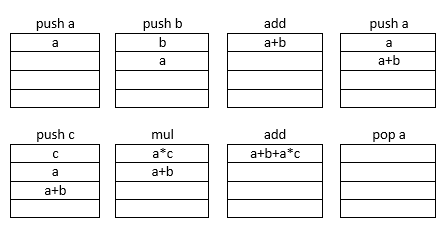
\includegraphics[width=\textwidth]{7_8}
\caption{Вычисления выражения $ab+ac\times +$ (в инфиксной нотации $a\hm+b\hm+a\times c$)}
\end{figure}
Рассмотрим вычисление постфиксной нотации в стеке. Стек не имеет адресных операций. В нем есть две операции с переменными: $push$ (положить) и $pop$ (забрать). Если необходимо положить значение в стек, то он кладется с помощью команды $push$ на вершину стека. При этом, все другие значения сдвигаются вниз. Арифметические операции ($add$ - сложить, $mul$ - умножить) выполняются с переменными (или переменной - зависит от арности операции), которые лежат на вершине стека.

%IN PROGRESS
\chapter{Программное обеспечение}
\section{������� ��}
�������� Microsoft ������� ������ doc (�������� �� �������� �� ���������) ������ � 2000 �. �� ����� ������������� ����������� ������� ��������� ����������� ������� ���������� ���� ��������. ��� ������������� ������ doc �� � ������ ������� - �� ��� ����� ������ (Microsoft Word - ������� ��) � ������ �������� ����� ����������� �����. �� ��� ��� ���������� ����� ������, ������� ���������� ������ � docx.
\\������� odt � docx ���������� XML. ���������� XML ������� - ����� ����� ����������, ����� ������, ���������� �����������. ����� ���������, ��� odt � docx ���������� XML, ���� ������� ������: �������� docx ��� odt ��������, ������� ���������� �� zip � ����������. ����� �������, ��� � �������� ��� ����� ����� ���������� xml.
\\���������� ������������ ��������� ������ � docx. � ������� doc ������ ������ ���� ���������. ������ ���������� ������������.
\\
\begin{center}
��������� ��������� Microsoft Office
\end{center}
\begin{itemize}
  \item ��� ���� � ����� (Word, Excel, PowerPoint, OneNote) $\approx$ 3000�.
  \item ��� ���� � ������� (Word, Excel, PowerPoint, OneNote, Outlook) $\approx$ 10000�.
  \item ���������������� (Word, Excel, PowerPoint, OneNote, Outlook, Access, Publisher) $\approx$ 20000�.
\end{itemize}
LibreOffice, OpenOffice, Calligra Suite = 0�.
\\
\\� 2010 ���� ��� ������ ���� � ���/��� 26300-2010, ����������� ������������� ������� �� ���������� ������ ���������� (Open Document Format - ODF). �� ��� ����� �� ��������, ��� ����� �������������� LibreOffice � OpenOffice. � ��������� ������� Microsoft Office ���� ��������� ����� �������.
\begin{figure}
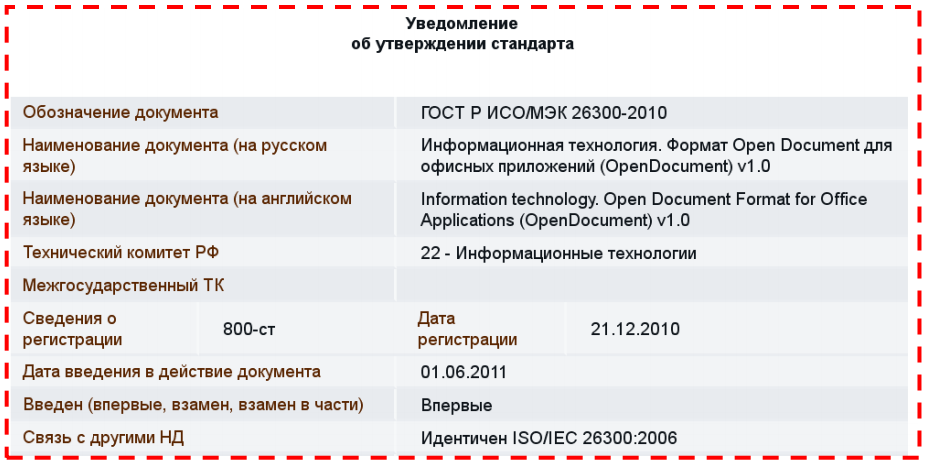
\includegraphics[width=\textwidth]{8_1}
\caption{���� � ���/��� 26300-2010}
\end{figure}
\begin{center}
\emph{ ODF}
\end{center}

\begin{itemize}
  \item ������������ ������������� ���������� ��������� �� 17 ������� 2010 �. �2299-� "� ����� �������� ����������� ������� �������������� ������ � ����������� ��������� ���������� �� ������������� ���������� ������������ ����������� (2011 - 2015 ����)"
  \item OpenDocument ��� ������������ ������ ����������� ������������, ������� ���������� ����������� ��������������� �� � ��������� ISO � �������� �������������� ���������.
  \item ��������� ����� ������������� �� ����� ������������ ������ OpenDocument ��� ���������� ������ ������������ ���������
����������� ����������.
  \item ��������������� ���� ������������� ������� OpenDocument ��������� ������������� ������������.
  \item ���������� ������� OpenDocument ������������ ����� ��� ������������ ����� �������������� ��, � ����� ������� ���� ������������� ���������� � �������� ���������. 
  \item ���������� ������� OpenDocument ��������� ������������ ���� ��������� ��� ������ ������������ �����������, �� �������� �� ����������� ���������� �� � ��� ������������� ��������.
  \item �������� ������ ����� ���������� ��-�� ��������� �������� ��������
\end{itemize}
���������� ODF:
\begin{itemize}
  \item ������������  ��������� �� ���������� ���������  �������� �������� ������������ �����������. �� ���� ������� ������ ����������� ����� ������������� ��� �������� ��-������, ��� ����� �������� � ��������������� ��������������� ������.
  \item ����� ������ ��������� ������� ������ ������� ���������� �������. �� ���� ������� ���������� ������� ������ ��������� ������� ��������� � ������� ����� ��� ����������.   
  \item ��������� ����������� �������, ��� Microsoft, � ����� ������� ����������� ��������� �� �����, ����� ������� ���� ���������� ������� OpenDocument � �������� �����,  �������  ������ ����������� ������� ����� ���������� OpenDocument. �����, �� ������ ���� ������������,  �� ��� ���������� ������� �������� ����� ������������� � ��������������� ������� � ����� ����� Microsoft ����� ��������� � ��������� ������ ��������, ��������� ������� �����, ��������� � ���� ��������� ���������� ���� ������������ � �������� OpenDocument.
\end{itemize}
������ �� �������������� OpenDocument �������� � ����:
\begin{itemize}
  \item \textbf{OpenDocument 1.0} (������ �������) OASIS (����. Organization for the Advancement of Structured Information Standards) ������������� ��������������� ��������� ISO/IEC 26300:2006. ���������� ISO/IEC 26300 � OASIS OpenDocument v1.0 2-� ������� ���������. ��� �������� � ���� ���������, ��������� ������������ �������� JTC1 ( ����. Joint Technical Committee 1) � �������� � ODF, HTML � PDF ��������.
  \item \textbf{OpenDocument 1.1} �������� �������������� ����������� ��� ������� ������� �����������. �� ��� ��������� � �������� ��������� OASIS �� 2007-02-01 ����� �����������, ��������������� 2007-01-16. ��������� ��������� ���� ������� 2007-02-13. ��� ������ �� ���� ���������� ������������ ISO / IEC, ������ ��� ��� ��������� �������������� ����������� ������ ODF 1.0, � OASIS �������� ��� �� ODF 1.2 � ��� ������, ����� ODF 1.1 ���� ����������. ������ ������� ���� ������������ ISO / IEC (�� ��������� �� ���� 2011 ����, �� ��� � "������ �������'' ��� ������ �������� 1- ISO/IEC 26300:2006/DAM 1) � ������������ � ����� 2012 ����, ��� ISO / IEC 26300: 2006 / Amd 1: 2012 - Open Document Format for Office Applications (OpenDocument) v1.1.
  \item  \textbf{OpenDocument 1.2} ��� ��������� � �������� ������������ OASIS �� 2011-03-17 � � �������� ��������� OASIS �� 2011-09-29. �� �������� � ���� �������������� ������� �����������, RDF-����������, ����������� ������� ������������ ������, ���������� �� OpenFormula, ��������� �������� �������� � ��������� �����������, ������������ ���������������. � ������� 2011 ���� ���������, ��� ����������� ������� OASIS ODF "����� ������ ������� �������������� ODF 1.2 � ISO / IEC JTC 1 ". � ��� 2012 ���� ������������ ISO / IEC JTC 1 / SC 34 / WG 6 ��������, ��� ����� ��������� ��������, ������� ���������� ODF 1.2 ��� ������������� JTC 1 ��� PAS ������������ ������� � ��������� �����.
\end{itemize} 
\subsection{�������� ���������� ������� ������}

\begin{table}[!h]
 \begin{tabular}{|l|c|c|c|}
\hline
��������  &   & ���������  &  \\
��������  & ����������� &  ��������� ��  & ��������\\
������ & & 2017 ���, ���. &  ���  \\
\hline
Google Docs, & ����� ���������� & &\\
������.����, & �� ��������� &  ��������� & �������� \\
������ Mail.ru  & �������� ������� & & \\
\hline
 &  ����� �������� ������� &  &  \\
 Microsoft Office &  ����������, ��������  &  5000-35000&  ��������\\
 & > 90\% desktop-���������  & & \\
\hline
LibreOffice,& ������ ��������� & & \\
OpenOffice, & �������������� &  ��������� & �������� \\
Calligra Suite & �������������� & & \\
\hline
 & ����� ���������� �� & & \\
iWork & �� ������� ����� Apple &  ��������� & �������� \\
\hline
 & ��������� ��������� & 5000 & \\
WPS Office & Microsoft Office &  (0 � ��������) & �������� \\
\hline
WordPerfect & ����� ���������� �� �����&  & \\
Office &  ������������ ����������� & 5000-25000 & �������� \\

\hline
OnlyOffice & ������������ ����������  & & \\
Feng Office & �� ������� � ��������� &  ��������� & �������� \\
  & ������� ������� & & \\
\hline
 \end{tabular}
\caption{�������� ���������� ������� ������}
\end{table}
� ������� ����������� �� ��� 30 �������������� ������� �������, � �������� ����������. ������������ �������  � �������  ����� Trends Google, ��� ������������� ������� �������� ������������� �� ����� ����.
� ������� ������� ������� ������ �� �������� ������������.
\subsection{��������� ������������ OO � MS Office}
\begin{table}[!h]
 \begin{tabular}{|l|c|c|}
 \hline
 �������� & Open Office Calc & Microsoft Excel \\
 \hline
 ����������� & 1 024 $\times$ 1 048 576  & 16 384 $\times$ 1 048 576 \\
 \hline
 ���-�� ������ & 104 & 16 777 216 \\
  \hline
 ������ � & �� 1 ������ 0001 �. & �� 1 ������ 1900 �. \\
 ������ & �� 31 ������� 9999�. & �� 31 ������� 9999�. \\
 \hline
 ���������  & met, pbm, pgm, ppm,  & cdr, emz, mix, pcz, \\
 ����������� & psd, ras, sbm, sgg, &  wmz, wpg, fpx,  \\
 �������� & svg, xpm, xbm &  drw \\
 \hline
 & ������ � MySQL. ������� & ����������� �������  \\
 ������ & �� ������ ������ & ������� � �������� \\
 & (Python, JavaScript) & ��������������  \\
  \hline
 \end{tabular}

\end{table}
\begin{center}
  \emph{Open Office Writer}
\end{center}
\begin{itemize}
  \item ������ ����������
  \item ����������� ����� ������� � ����� ���������
  \item �������������� �������� ��������� ������
  \item ����������� ��������� (�� �������, ��������, �����������, ������������)
  \item �������� ���������� ������ ���������� ������ � ����� ���������
  \item ���������, �������, ���������� ������� ������������� ����������� �������
  \item ������������ ���������� ����� ������� ��������� � ����� ���������
  \item ��������� ���������� � ����� ���������.
  \item ������������������ ����������� ��������� ���������� � ������� � �����������.
\end{itemize}
\begin{center}
  \emph{Microsoft Word}
\end{center}
\begin{itemize}
  \item ���������� �������� ��� ����������� �������� ���������� �������� �����
  \item ������������� ������ � ����������� �����
  \item ��������� ���������� ������� � ���������
  \item ������� ������������������
\end{itemize}
���� ���������� \emph{������������������} OpenOffice Writer � Microsoft Word, �� Writer �������� �������������� � ��� ����.
\\���� ���������� \emph{������������} OpenOffice � Microsoft Office, �� Microsoft ������� ��������, ��� OpenOffice (MS Office 2010: 17 ������ � 0 ������������� �����������, � OpenOffice 3.2.1: 163 ����� � 18 ������������� �����������). ���� �� ������ - ����������� ���������� �� ���������� ��������.
\subsection{��������� ������ � ��������}
\begin{itemize}
  \item 1-� ������ - �������������� ������� ��� ������.
  \item 2-� ������ - �������� ���������� ������ �������� ���������.
  \item ��� ���������� ��������� ������� ��, ��� ����� ��������. � ��� �� �������� - ��������.
  \item ������ ��� "������ ������ 14pt"\, "��������� Times New Roman"\, "������������ �� ������" � ��� �����.
  \item ������� ������ �����: "���������"\, "��������� $n$-��� ������"\, "�������� �����", � ��� �����.
  \item �������� ������ ��������� ���������� � ������������ ��������� ��������� � �������� ������� ������.
  \item ��� ����� ��������� �������� ��������, (������, ���������, � ��� �����) ��������, ����� �������� ��� �����, ����� ��������� ���������������� �����.
\end{itemize}
\subsection{���������}
\textbf{���������} (����. "\emph{��� �����}") ��� ������������ - �����, ������������ ��� ��� ����� ��� ����� ��������.
������������ ���:
\begin{itemize}
  \item ������������ �������.
  \item �������� �������� ������ �� ������ �����.
  \item ������������ ���������� ���������.
\end{itemize}
\begin{description}
  \item[Microsoft] ����� [��] ��� ���� ������ ����������� �����, �� ����� ���.
  \item[KDE] ������� �������������� ����� �������� ���� ������ ������ ������� ��������� ���������.
  \item[Gnome] � ����� ��� ��� �� ������? ��, �� ��������� ���������!
\end{description}
\subsection{��������������}
\textbf{Lorem ipsum} - �������� ������������� ������-"����".
\\\textbf{"����"} - ����� �� ������� ����������, ���������� ��������, �������� ������������� �����, ����������� � ����� ��������.
\\
\\Lorem ipsum ������������ ����� ���������� ������� �� ������������ �������� �������� "� �������� ����� � ���", ����������� � 45 ���� �� ����� ��� �� ��������� �����. ������� ���� ����� ��� �������� ��� ������ ��������� �������� ����������� ���������� � XVI ����.
\\
$$=rand(m, n)$$
���:
\\$m$ � ���������� �������;
\\$n$ � ���������� ����������� � ������ ������;
\\��� ��
$$=lorem(m, n)$$
\subsection{��������� ���������}
��������� ��������� �������� �� �������� ������� ����� ��������� ���������, ������� ������� �������� ������ � ������������ ���������:
\begin{itemize}
  \item ������ �� ���� ������������ �������� � ������.
  \item �������� ��������������.
  \item ������� ��� ����������� ������.
  \item ������ �������������� ���������.
  \item ������ ��������� (������� ���������, ������� ������ ������������ �������).
\end{itemize}
\section{��������������� �� ��� ����������������}
\begin{itemize}
  \item �������������� �������� ������������ ��� ��������� (doxygen).
  \item �������� ������ (SVN, Git, Mercurial).
  \item ���������� ��������� ������ ��������� ������ (bug tracking system).
  \item ������������������ ������������ ���� � ����������������.
\end{itemize}
\subsection{������������������ �������� ������������}
����� ��������� ������� ��� ������������� �������� ������������ ������������ ����������� �� �/�++ - ��� \emph{doxygen}. ������������ � KDE, IBM, AbiWord, Adobe, DC++, Qt, \dots
\\��� ������ � Doxygen ����������� ��� (� ������������ ���������� ����������� ���������, � ���������� ���� ����������� ����������������� � ������������).
\\
\\����� ��������� ����������� ��������� ������: �� ����� �������� ��������� ������������. ����� ����, � ������������ ��� �������� ������� � ����� ����������� ������ ����������� � ���������.
\subsection{������� ���������� (��������) ��������}
\begin{itemize}
  \item \textbf{������-��������� (����������������)}: CVS, Subversion, Microsoft SourceSafe, Perforce, VSS
  \item \textbf{��������������:} Mercurial, git
  \end{itemize}
\emph{������� ������}: ������� ������, ������� �������� ������������, ������������� �� ���� (release ������) � ������ ��� �������������, � ������� �������� ������ ��������� (������� ������������ �� ��������). ��� ���������� ��� ����, ����� ������������� ����� ������ (������� ���������, �����������), �, ��� �������������, ���� ����������� ���������� �� ������ ������. ���������
\\������������ Git ��� SVN: ������� ������ � ������� ����������� �����, �������� ���� ������� ��������� ������ �������. ������� ���������� ������ ��� ���������� ������.
\subsection{��������� ���� ������������ ������}
\begin{description}
  \item[�����������] ������� ������;
  \item[�������� �������] ��������� ����, ��� �������� ������;
  \item[�����������] ���������� ��� ���������, ������ ������ ��������� (�����; ��� ������ ����������; ������ �������������);
  \item[�����������] ���������, ���� �� ���������� ������.
\end{description}
\subsection{������������ ������������ �����������}
����� ��������� ���� ������: JIRA, Redmine, Bugzilla, TrackGear.
\begin{center}
  �������� ������
\end{center}
\begin{itemize}
  \item ��� ������� �� ������;
  \item ���� � ����� �����������;
  \item ����������� ������;
  \item �������� ����� ��������������� ������;
  \item ������� ������ ������.
\end{itemize}
\textbf{������������������ ������������ ������������ �����������} - ����� �������� ������������ �� ����� �������� �������� � �������� ���������� ������������ �����������.
\\��� ���������� ����������� �������� ��� ���������� ������ � �������� ����������� ����������, ��� �������� ��������� ����� ������������ � ��������� ��� �������.
\begin{center}
\textbf{�������� ��������� �������������� ��� ������������:}
\end{center}
\begin{itemize}
  \item JUnit � ������������ ���������� ��� Java
  \item NUnit � ���� JUnit ��� .NET
  \item xUnit � ������������ ���������� ��� .NET
  \item TestNG � ������������ ���������� ��� Java
  \item Selenium � ������������ ���������� HTML
  \item WatiN � ������������ ���-����������
  \item TOSCA Testsuite � ������������ ���������� HTML, .NET, Java, SAP
  \item UniTESK � ������������ ���������� �� Java, ��.
\end{itemize}
\section{��������}
\textbf{�������� �� ����������� �����������} � ��� �������� ����������, ������������ ������������� � ��������������� ������������
�����������, ����������� ��������� ������.
\begin{description}
  \item[������������� ��] $\Rightarrow$ �������� �������� ���. ����� ���� ������� � ����������.
  \item[��������� ��] $\Rightarrow$ �������� �������� ���. ����� ���� ������� � ����������.
  \item[������������ �� ] $\Rightarrow$ �������. ����� ����� ��� ��������, ��� � �������� �������� ���.
  \item[���������� ��] $\Rightarrow$ ����������. ����� ����� ��� ��������, ��� � �������� �������� ���.
\end{description}
\begin{center}
������������� �������� �� ��������� ��
\end{center}
\begin{itemize}
  \item\textbf{������������ �������� (BSD)}: ����� ������ � ���������.
  \item\textbf{�������� (GPL)}: ����� ������, ������ ���������.
\end{itemize}

\begin{wrapfigure}[12]{l}{3cm}
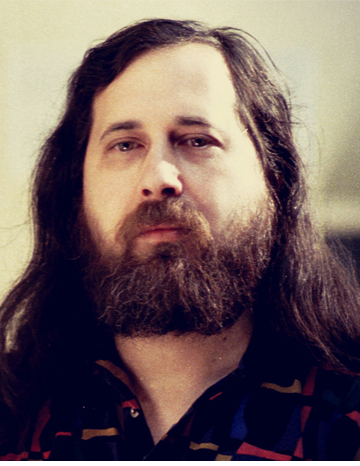
\includegraphics[width=3cm]{8_2}
\begin{center}
\footnotesize{������ ������ ��������}
\\\footnotesize{$\mbox{���.} 1953$}
\end{center}
\end{wrapfigure}
���������������� �������� �� �������� ��� �������� ������ ������ ��������. �� � ������ ������ �������� GNU (General Public License).
\\����� ����� 70 �������� �� �������� ��������� �� (���������� �� opensource.org). ����� ����������: Apache License, BSD license, GPL, LGPL, MIT license, MPL.
\subsection{������� �����, ��������������� ��������� ��}
��� ��� ������������� 4 ������� �����:
\begin{itemize}
  \item ����� �� ������ ��������� � ����� ����� (������ ���� ��� �� ������� ���� ����� ��������� ��� ������������).
  \item ����� �� �������� ��������� � ��������� ���� ���������
  \item ����� �� ������� ��� ���������� ��������������� ���������.
  \item ����� �� �������� ���������.
\end{itemize}
���� ����������� �������� ������������ ���� ��������� , �� �� ��������� ��������, �� ��������� "����� ���������� �����������":
\begin{itemize}
  \item ����� ���������� ��������� �� 1 ���������.
  \item ����� ��������� ��������� �� 1 ����������.
  \item ������ ���������� ��������� �� ������ ����������.
  \item ������ �������������� ���������.
  \item ������ �������� ��������� 5 ��� (�.4 ��. 1235 �� ��).
\end{itemize}
\subsection{����������� ��������� ��������� ��������}
\begin{center}
  \textbf{GNU GPL}
\end{center}
\begin{itemize}
  \item ��������� �������� �������� ������ � �������� ��, ��������� ������ ��� �������� (copyleft $\textcopyleft$).
  \item ��������� ������������ ���������� GNU GPL-��������� � ��-GNUGPL ������������ (dll).
\end{itemize}
\begin{center}
  \textbf{GNU LGPL}
\end{center}
\begin{itemize}
  \item ����������� ������������ ���������� � ��������� ������������.
  \item ��������� ������������� ���� � ������ ��.
\end{itemize}
\begin{center}
  \textbf{MPL (Mozilla public license)}
\end{center}
\begin{itemize}
  \item ����� ������������ �������� ������ � �������� ��, ��
���� �������� � � ��������� ������� � ����������.
\end{itemize}
\begin{center}
  \textbf{BSD License}
\end{center}
\begin{itemize}
  \item ����� ������������ �������� ���� � �������� �� ��� �����������.
\end{itemize}
\subsection{��������������� �� ��������� ��}
\begin{description}
  \item[���������������� ��������������� �� ��������� ��] ������ 7.12 ���� ��: ��������� ��������� ���� ��� ������ �� ����� �� 100 000 ������:
  \begin{itemize}
    \item ����� �� 2 000 (���������� ����)
    \item ����� �� 20 000 (����������� ����)
    \item ����� �� 40 000 (����������� ����)
  \end{itemize}
  \item[��������� ��������������� �� ��������� ��] ������ 146.2 �� ��: ���������� ������������� �������� ���������� ����� (� �.�. ������������, ��������) ��� ������ �� ����� �� 100 000 ������:
\begin{itemize}
  \item ����� �� 200 000 �.
  \item �������������� ������ ������ �� 2 ���
  \item � ����� ������ �� 2 ���
\end{itemize}
 ������ 146.3 �� ��: ���������� ������������� �������� ���������� ����� (� �.�. ������������, ��������) ��� ������ �� ����� �� 1 000 000 ������:
  \begin{itemize}
    \item ����� �� 500 000 �.
    \item ����� ������ �� 6 ���
  \end{itemize}
  \item[��������� ��������������� �� ������� ��] ������ 146.1 �� ��: ���������� ���������, ���� ��� ��������� ������� ����� ������:
 \begin{itemize}
   \item ����� �� 200 000 �.
   \item �������������� ������ ������ �� 1 ����
   \item ����� ������ �� 6 �������
 \end{itemize}
  \item[����������� ��������������� �� ��������� �������� ��]  ������ 1301 �� ��: ��������� ���������, ���������������� � �������������� ����:
  \begin{itemize}
    \item ����� �� 5 000 000 ���. � ������ ���������� ��
    \\\textbf{����}
    \item ���������� ���������� ������� ���������� ��
  \end{itemize}
\end{description}
\section{Visual Basic for Applications}
\textbf{Visual Basic for Applications} (VBA, Visual Basic ��� ����������) � ������� ���������� ���������� ����� ���������������� Visual Basic, ���������� � ������� ��������� Microsoft Office (������� ������ ��� Mac OS), � ����� �� ������ ������ ����������� ������, ����� ��� AutoCAD, SolidWorks, CorelDRAW, WordPerfect � ESRI ArcGIS. VBA ��������� � ��������� ���������������� ����� ���������������� ������������������ �����-������, ����� ��� WordBasic.
\\
\\\textbf{������} � ���������, ���������� �� ���������� ��� ���������� ���������� ����� ����������������, ������� ����� ��������� �� ������� ������������. ��� ��������� ����� ��������, ��� � �� ������ ����� ����������������. ��� ��������� ���������������� ������������� ��� ������� �������� ������������, ������� ����������� � ����������� ����������� ���������� ����������. ����� ������� ����� ��������� ����������� ����������.
\\
\\������������� �������� ������������ ������ ����������� � ��������� ��������� ����� ����������������. ������ ����������� ��������� ���������� ��������� �������������, �� ������� ���� ��������, ���������� ���� �������� ��� ����������� �� �������������� � ������. �������� ������������ ������������� ����������� � ������� ����������� ����� ����������������. 
\\
\\�������������� ������ ������� ����� ������ ������������, ������� �������� ������������ � �������� ����� ���������������� �������� � ������� ��������� Microsoft Office Visual Basic for Applications.
\subsection{��� ����������}
\begin{itemize}
  \item ���������� � ����� ���������� ��������.
  \item �� ����� ��������� �������, ����� ������� �������� (+, -, *, /, \#, \$, \%, \&, !, <, >, = � ��� �����).
  \item �� ����� ��������� 254 �������� � �����.
  \item ������ ���� ���������� � ����� ������� ��������.
  \item �� ����� ����������� ����������������� �����.
  \item �� ��������� ������� ����: MyNumber = mYnUmBeR.
\end{itemize}
\subsection{���� ������}
\begin{minipage}{\textwidth}
\centering
\begin{tabular}{|l|c|c|c|}
\hline
��� ������ & ������������� & ����������� & ������������ \\
& ������, ���� & �������� & �������� \\
\hline
Byte & 1 & 0 & 255 \\
Boolean & 2 & False & True \\
Integer & 2 & -32768 & 32767 \\
Long & 4 & -2147483648 & 2147483647 \\
Date & 8 & 1 ������ 100 �. & 31 ������� 9999 �. \\
String & ����� ������ & 1 & 65400 \\
Variant & \multirow{2}{*}{16} & & \\
(�����) & & & \\
Variant & 22 ����� + & & 2147483647 \\
(������) & ����� ������ & & �������� \\
\hline
\end{tabular}
\end{minipage}
\begin{center}
 \textbf{���������� ����������}
\end{center}
\begin{enumerate}
  \item \textbf{�������}:
  \\sum = 100
  \\� ������ ������ ������������� ��� Variant. ��� ���������� ���, ���������� ��������������.
  \item \textbf{�����}:
  \\Dim sum As Integer
  \\\emph{������������}:
  \begin{itemize}
    \item ��������� ������� ��������.
    \item ��������� ��������� ������ ������.
    \item ����� ���������� ��������� ������.
   \item �� ��������� ������� �� �������� ������ (��������, ��� �������� ���� �� ������).
  \end{itemize}
  \emph{����������}:
  \begin{itemize}
    \item ���������� ������.
    \item ��������� ������������ ������ ����������.
  \end{itemize}
\end{enumerate}
\section{\TeX}
��� �������������� �������� � ����������� ��������� ������: ����� �� ������� ������������ ��������� �� ������ � ����� � ������ ���������� � � �������� ����. �� ���� ���� ���������� 2 ���������:
\begin{itemize}
\item \textbf{WYSIWYG} (����. \emph{What You See Is What You Get} - "��� ������, �� � ��������") - �������� ���������� �������� ��� ���-�����������, � ������� ���������� ������������ � �������� �������������� � �������� ����������� ������ ������� �� �������� ���������, ������� ����� ���� �������� ����������, ���-��������� ��� ������������. � ��������� ����� ��� �������� �������� ����� ������ ������������ ������� "���������� ��������". (������: Microsoft Word)
\item \textbf{WYSIWYM} (����. \emph{What You See Is What You Mean} - "��� ������, ���� ��, ��� ������ � ����") - ��������� �������������� ����������, ��������� ��� ������������ ����� ���������������� ��������� WYSIWYG. � WYSIWYM ��������� ������������ ������ ������ ���������� ��������� ��������� � ���������� �������. ���������� ���������, ��� �������� ������� ��� ��������� �� ��������� ��, ����, �� ������ ������, �������� � ��������� ����. ����� ������� ����������� ������ ������������� ���������� ���������
�� ��� �����. (������: \TeX)
\end{itemize}
\textbf{\TeX} - ������� ������������ �������, ������������� ������������ ����������� ����������� ��������� ������ � ����� �������� ������������ ����������. � ��� ������ �������� ��� ��������������� ����������, ��� ������ � ������������� ��������. ����� ������ \TeX ������������ � $\pi$, ����� ��������� ������ - � ����� $e$.
\subsection{��������� \LaTeX � WYSIWYG �����������}
\LaTeX (������������ �����) � �������� ���������� ����� ��������������� (��� ����������) ������� ������������ ������ \TeX, ������� ��������� ����� ������� ����������. ���������� ����� ��������� � 1984 ���� � ������ � ��� �����.
\begin{table}
\begin{tabular}{|l|l|l|}
\hline
�������� & \LaTeX & MS Word, \\
 & & LibreOffice Writer \\
\hline
 ������& �������� ��������� & ������������ ����� \\
� ��������� &  ������������� ������ & �������� � ���������.  \\
 &  &  ����� ������� \\
\hline
 ������������& ��������� ��������� & ���������� ��������� \\
 ������& ��������, ������&  WYSIWYG ��������, \\
&  ��������� �������-& ��������� ���������� \\
&������ ������� & ���������� ���������� \\
\hline
����� ���������& �������& ������ \\
\hline
���������& �������� �������& �����������  \\
������� ������& ����������& ���������� �������� \\
\hline
���������&���������&LibreOfice ��������� \\
\hline
��������������&���, �����&����������� ���������� \\
�������& �������������� &����������� \\
\hline
������� � &\multicolumn{2}{l|}{����������� ���������� ������� ��� } \\
 ������ �������& \multicolumn{2}{l|}{�������� �� docx � tex � ������� �� ����������} \\
\hline
���������� �& ����� ������:& \\
�������. �����������& ���������� ������� & �������\\
\hline
�������������&������ ������������& ��������� ������\\
����������&������ �������&  ������� ��������� \\
 &���������� ��������&  docx (odt) \\
\hline
������������& &�������������� MSW\\
������ � �������&���������������&  �� ���������\\
\hline
���������� & ����&����� \\
�����������������&(������, ������������ �& (����������� \\
�������������&������. ������������)& ����������� �����) \\
\hline
�����-�������-& & ����������� \\
�������� ��&����� �� & ���������� ��  \\
 ��� �������������� & &  � �������� GUI \\
\hline
�����-�������-&�������� &�������� ��� \\
��������&������������� & ���������� ������ \\
������� ����� &������ ���������� & \\
\hline
�������� ����������&����������&�������� ��\\
� ����������&(������� hunspell)&��������� \\
\hline
�������������&����������� (�����& ���������� ���������  \\
������. �������� &������������ �������) & �������� \\
\hline
������ � & ��� �����������&���������  \\
�������� �������& & "���������" \\
\hline
���������& �� ������ ����������& �������� ��-�� \\
 &PDF ����& �������������� ��������� \\
\hline
\end{tabular}
\caption{��������� \LaTeX � WYSIWYG �����������}
\end{table}
\section{��������}
\textbf{������� (������-�������)} - ������������� ���-�����������, ���������� ������-������ ��� ����������� ����� ��������. �� ����� ���-����������� ������ �� ���������� ��������� � ������ ����������, � ����� ����� ���� �������������� ����� �������� ����������� ������������ ����������, �������������� �� ���������� ������� ���������, ��� ����� ���-����������.
\\1988 �. � ��������� ������ IRC (����. Internet Relay Chat).
\\�������� 1990-� � ��������� � ��������������� IM (Instant Messaging).
\\1998 �. � ����������� ��������� ����� "Webinar" ������ �. ������ (Eric R. Korb).
\begin{center}
  ���������� ��������� ���������� ��� ���������
\end{center}
\begin{itemize}
  \item GoToMeeting
    \begin{itemize}
    \item ������� � 2004 ���� ��������� Citrix Online.
    \item �������������� ��: Macintosh, Microsoft Windows
    \item http://www.gotomeeting.com/
  \end{itemize}
  \item StartMeeting
    \begin{itemize}
    \item ������� � 2011 ���� ��� start-up.
    \item �������������� ��: Microsoft Windows
    \item http://www.startmeeting.com/
  \end{itemize}
  \item Team Viewer
    \begin{itemize}
    \item ������� � 2005 ����.
    \item �������������� ��: Windows, Mac OS, Linux, Android, Apple iOS, Windows Phone
    \item http://www.teamviewer.com
  \end{itemize}
\end{itemize}

%\chapter{Структура и принципы функционирования Компьютера}
%���� �������� ������� ��������� ���������� �����.
\\������ (����� �������������� ���������) ��� \textbf{�������� ��� ������������ � ���������}. ������� ��� ��������� ������� (\emph{1592 - 1635}) � 1623 ����.
\\������ ��������� ����������� � ������������ ����������, � ����� �������� ��� ������ ������������� �����������. ������ ���� - �������������� ����������� ������ - ����������� ����� ���������� �������� �������. �� ������ ��� ������� �������� � ������� ������� � ��������������� ��������� ������ - �����. ����� ������ ��� ����, ����� ���������� ������� � ��������� ������ (������������ ���������� �� ������� ����� ������� �������, ����� ���� ��� ���������� ����������� ������� ������� ����� ������). ��� ��������� ���������� ��������� ������� � �������� �������. �������� ���� ���������� ����� ���� ����� ��� ������ ����������� ������, ��� ���������� �����. ��� ������������ �������������� ����������, ��� ������� ����� ���������� ����� ���� � "�����������" �� ��� ��������� ���������.
\\������ �������������� ������� ��� \textbf{�������� ��� ������������ � ��������� "������\'���"}. ������� ��� ���� ������� (\emph{1623�1662}) � 1642 ����.
\\������ ������� ������������ ����� ������������ ���������� � ���� ������ � ��������������� ���������� ���� � ������ ������������. ������������ ����� ��������� � ������ ��� ������ ���������������� �������� �������� ���������. �� ������ �� ���� ���������, ����������������� ������ ����������� ������� �����, ���� �������� ������� �� 0 �� 9. ��� ����� �����, �������� �������������� �� ��������������� �����. �������� ������ ������, ������� ��� ������ 9 �������� ���������� �� �������� ������, ������� �������� ������ �� 1 �������.
\\��������� ��� \textbf{���������� ��������}, ������� ��������� �������� ��������, ���������, ������� � ���������. ������� �� ������� ��������� ������� (\emph{1646 - 1716}) � 1673 ����.
\\�������� ����� ����������� ��� ������ ��������� ���� � ������ �����, ��� �� ��� �� "���������". ����������� � ����������� ���������� ����� � ����������� ��������, ����������� ������� ����������� ������ (� ����������� ��������� ������ - ��������), ��������� �������� ������������� �������� ��������, ��� ������ ������� ����������� ������� � ������������ �����. ����������� ����� ��������� �������� ����������� �������������.
\\���������� ������������ ���������� ����� \textbf{���� �������� ������������� ������������� �������������� ������}, ������� �������� ������ ������� (\emph{1791 - 1871}) � 1823 ����.
\\� 1822 ���� ������� �������� \textbf{����� ���������� ������}. �� ������ ���� �������� �� ������ �������� ���������. ����� ������ ���� ��������� ������������ � �������� �� ��������� ���������� � �������. � ��� �������������� ���������� ������� ���������. ��� ����������� 18-���������� ������� � ��������� �� �������� ����� ����� ������� � ������������ �������� ���������� 12 ������ ������������������ � 1 ������. ����� ���������� ������ ����� ������� �������� ����������� 7-� �������.
\\� � ��� �� 1822 ���� ������� ��������� � �������� \textbf{������� ���������� ������} ��������������� ��� ������������� ���������� ����� ������������� ������� ������������ � ���������� �������� ���������. ����������� ������������� ������������� � ����������� ���������� � ������������������ ������� ��������� �� ������������� ��� ������ ��� �������� ������������� �������������� ������. � 1823 ���� �� ��������� � ��������������, ������, � 1842 ���� ����������� ���������� ������������� ������ � ������ ��� � �� ���� ���������. �� ��� �������� �������������� ������� ����� �������� ������: ���� �������� ������������� �������������� ������. � ������ ���������� ����� ������� ������ �������������� ���������� (��������� �� "���������"), �������� ������, ������������ � ������ ����� ("�����"), � ���������� �����-������, ������������� � ������� ��������� ���� �����. ���������� �������� ����������� ������ ����� �������� ��������, ���������, ������� � ���������. ���������� ���������� ��������� ��������� ������ �� ������ � �������������� ���������� � �������. �������� ���������� ����� ���� ������������ ��� ��� ����� ������ � ������, ��� � ��� ���������� ����������� ����������, ���� ������ ���� ������������.
\\��������� ������ � �������� �������������� ������� ���� \textbf{������������������� �������������� ��������� ��� �������� ���������}, ������� ������� ������ �������� (\emph{1860 - 1929}) � 1880 ����.
\\���������� ������������� ��� �������������� ��������� (������������ � �������������) �������� � ��������� ����������, ���������� �� �����������, � ������� ����������� �� �������� ����� ��� ����������� ������. ��������� � ������� ����������� ������� ����������������� ������������� �������� � ���������. ������ ���������� ������������� � ������������ � ���������� �� �������������� ������ ����������.
\\� 1911 ���� ������� ���������� ������ (\emph{1863 - 1945}) ������� \textbf{���������� �������� ���������������� ���������}. �� ������������ ������������ ���������������� ���������.
\\� 1919 ���� ������� ���������� ���������� (\emph{1884 - 1937}) �������������� \textbf{���������� �������������� ������ (���)}. ��� ���� ������� ��� ���������� ������ ������������ ��������� ������� ��� ������ �������-��������������� �������������, ������� ���������� ���������� � ��� �� 1919 ����.
\\\\������� ��������� ������ ����������� ������ � �������� ���� ����������� ������ ������ ������������ ������. ������� �������� ������ ��������� � ����� ��������� ����������� ��������������� ����������. ���, ���������� ������������, � ��������, �������� ������������ � ������������� ������� ����������� ��������. �� ����� ������������ ����������������� ��������, �� ���������� ��������� ��� ��������� ������ � ������������ ���, ��� ��������� ���������������������� ��� �����. ��������� ���������� ��������� ��� ������ ���� ��������� ������� ����������� ������ �� ���������, � � ����������� ������� ����������. �������, �������������������� ������ ������������ ������ ��-���� �����������, ������ ��������� ��������� ������ ������ ������ �� ���������� ����� ������������, �������������� � ����������� ������ � ��������� � �. �.
\\\\�� �������� ���� �������� ������������ �������� � ����� ������. �� ������� � ��������� ������������� ����������, ���������� �� ������� ����������� ����������, � ������������� ��������������� �������� ��� �������� ���������� ����������, ���������� � ���������, ����������� ��������� �������� �������������� ������ � ����� ��������� ������. ���� � ��� �� ������ � ������������ ������ � ���������� ������ ����� ������ ��������� ����� ��������.

\section{��� ����� ��� �������}
\begin{minipage}[l]{3cm}
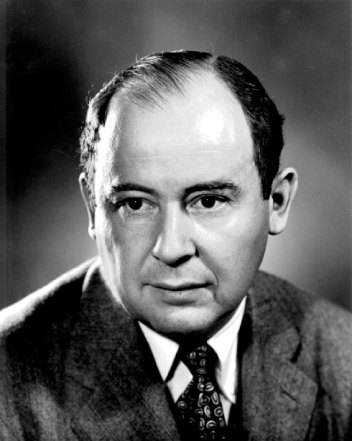
\includegraphics[width=3cm]{9_1}
\begin{center}
\footnotesize{���� ��� ������}
\\\footnotesize{$1903 - 1957$}
\end{center}
\end{minipage}
\hfill
\begin{minipage}[r]{7.5cm}
� 1930-� ����� �������� ���������� ����������� ��� ��� ������-������� ���������� �� ������ ������������� ���. � ���������� ����������� ����������� ����������� � ������������ ����������� (� ��� ����� � ���� ��� ������). �� ������� \ref{tag:EVM_von_Neumann} ��������� ����� ���, ������������ ��� ��������.
\end{minipage}
\\
\begin{figure}[h]
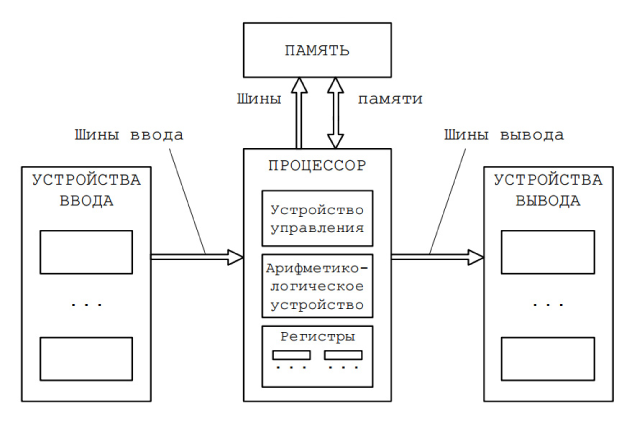
\includegraphics[width=\textwidth]{9_2}
\caption{����������� ����� ��� ��� �������}
\label{tag:EVM_von_Neumann}
\end{figure}
\subsection{���� ��� ��� �������}
\begin{itemize}
  \item \textbf{���������} - ����������� �������� ���������� (���� ��������), ������� ����� ����������� ����������� ���. � ������ ���������� ������:
      \begin{itemize}
        \item ���������� ���������� �������� ������ �� ������ � �� �����������;
        \item ����������-���������� ����������, ������������ �������� ��� �������;
        \item ��������, �������������� ��������� �������� ������ � ��������� ����������;
        \item ����� ��� ���������� � ����� � ������������ ������ � �����-������.
      \end{itemize}
  \item \textbf{���������� �����} ������������ ���������� ������ � ��������� ���������� � �� ������������� � ����� ������������� ��������, �������������� ������� ������������ ��� (����������� ��� �������) (����, ����������, ������).
  \item \textbf{���������� ������} ������������ ���������� ��������� ������ � ��� � �����, ������� ��� ����������� ���������� ��������� (�������, �������) ��� �������� (DVD-������, �������). ��� ������������� ��� ������������ ����������� ����������� �� ���������, � ������� ��� ���������� ����� ���� ����� ������� � ��� ��� ���������� ��������� (����������, ��������� �����, ��������� ���� � �. �.), ��� �������� ����������� �� �������������� ������ ������������ ������� (��������, ������). 
  \item \textbf{���������� �����-������} ������������ ��� ��� �������� ������, ��� � ��� �� ���������� (������� ����, ������).
\end{itemize}
\subsection{�������� ������ ����������� ��� �������}
�����, ��������� � ��� ������ � 1946 �. � ����� "��������������� ������������ ����������� ��������������� ������������ ��������������� ����������"  ������� ��������:
\begin{itemize}
  \item \textbf{������� ��������� �����������} - ��� ����������, ����������� � ���, ���������� � ������� �������� ��������.
  \item \textbf{������� ������������ ������} - ��������� � ������ �������� � ����� � ��� �� ������. ������� ��� �� ���������, ��� �������� � ������ ������ ������ - �����, ����� ��� �������. ��� ��������� ����� ��������� ����� �� ��������, ��� � ��� �������.
  \item \textbf{������� ������������ ������} - ���������� �������� ������ ������� �� ��������������� �����, ���������� � ������������ ������ ������� �������� ����� ������.
  \item \textbf{������� ��������� �����������} - �������������� � �������� ������ ���������, �����������, ������ ������.
  \newpage
  \item \textbf{������� ������������ ����������}:
  \begin{enumerate}
    \item � ������ ���������� ���������� ����� ������ ������� ��������� (������� ��������� � ����������� \textbf{������� ������}), ����� ����� ��������� ��������� ���� �����.
    \item ����� ���������� ������� ��������� ����������� �����, �������� � �������� ������, �� ����� ������ ��� ����������� �������, ����� �������� ����� ��������� �������. ��� ����� ��������� ������� ������ �� \textbf{���������������} ������������� ����� ������.
    \item ���������� ����������� \textbf{������� ���������}, ������� ����� �������� � ���� ����� ��������� �������. ����� ���������� ����� ������ ��������� ����� ������ ��������� � ������� ������. ��� ����� ��������� ������� ������ �� \textbf{�����������������} ������������� ����� ������.
  \end{enumerate}
\end{itemize}
\section{������������� ���������� ���}
\textbf{����������� ���} - �������������� ��������� �������������� ������, ������������ ���������� ��������� ���������� � ���������� ������ �������������� ���������� � ������ � �������� �������������� ����������� ������� � ������������ �����������. \textbf{������������ ���} ������������, ��� ������ � ���� ��� ���������� ��������� � �������������� ������ � ������ ���������� ��������� �������������� ����������� ������� � ������������ �����������.
\\� 30-� ����� ������������� ��� �������� ������������ � ������������� ������������� ����������� ����������� ��� ��� ������-������� ����������. �������� ���������� ������������� ������������ (����� ��������� ��� ����������� ��� �������, ��������� ��� �� ����� ������������, ������ ��������������� ����� �� �����������), ��� ��� ��� ���� ����� � ����������. ����������� ����������� �������������� ��������� ������ �. �. �������.
\\� ��������� ����� ���������� ��������������� � ��� �������� ��� 2 ���� �����������: \emph{������������ (������������)} � \emph{�����������}. ��� ��� �������� 2 �������� ���� ���: ����������� ��������� � ������ ����������. �������� ����������� � ��������� ������:
\begin{itemize}
  \item \textbf{������������ �����������}: ��������� � ������ �������� � ����� ������� ������ (����������) � ���������� � ��������� �� ������ ������ ����� (����). ����� ����������� (���������������), �������� ����������� ��������.
  \item \textbf{����������� �����������}: ��������������� ���������� ��������� � ������ �������� (����) ��� ������ � ������. ����������� ������������� ������ � ������� � ���������.
\end{itemize}
� ����� ��������� ��������, ������������ ���������� �����������, ����� ������: ����������� ����� ���, �������� � ������� ������� � ��������� ���� ����������� �����, ����������� � ����������� ����������� ���, ����� � ����������� ���������, ����������� ������ � ������� � ���������, ����� � ������ �������� ������ ����������, ������� ������������� � ������� ������, ������� ��������� ����������. \\
\\�� ������������� ��������� � �� ���������� ����� ���������� ��������:
\begin{enumerate}
  \item \textbf{�� ����������� ����������� � �������� ����}: 8-, 16-, 32-, 64-, 128-���������.
  \item \textbf{�� ������������ ������ ������ � ���������}:
  \begin{itemize}
    \item CISC � Complete Instruction Set Computer
    \item RISC � Restricted (Reduced) Instruction Set Computer
    \item CRISP � Complex-Reduced-Instruction-Set Processor
    \item VLIW � Very Long Instruction Word
  \end{itemize}
  \item \textbf{�� ���������� ������������}: ����������������, �����������������, �����������, ������������.
  \item \textbf{����������������� �� �������� �������������� � �������}: ������������ ����������������� (SMP), ���c����-������������ (MPP), ��������������.
\end{enumerate}
���������� ��������� ����������� ������ ������ (������� \ref{commands}):
\begin{itemize}
  \item \textbf{����������� �����������} - ������ ���������� ���������� ����������� ������ (��������) ��� �������� ������������� �����������.
  \item \textbf{�������������� �����������} - ���������� ���� ������� (�����������), � ������� �������� ���������.
  \item \textbf{�������� ����������� (MISC } - Minimal Instruction Set Computer) - ������� �� ����� ���������.
\end{itemize}
�������� �������� (�������� � ���������) ������� �� ������ ��������������� ���������� ���������� ��������: ������� ���� ���������, ����� ���������� � � ����������, �, �������, ���������� ����������. ����, ������������ �  ������������� �������, ����������� � ���������� ���������� ����� �������� ������ � ������. � ������ ���������� ������ ����� I� ��� �������� ���������� �������������� ��������������� �����, � ��� ������ � ������� � ������������������� ��������. ��� ��������� ������������ ���������� � ������������ ������� � ������, ��������� ���� ����������� ���������� ����� ��������������.
\\��������������� ����� ���������� ������� � ������ ����� ���� ��������� ���������� � ������� ���������. ��� ���������� ������� �������� ������ � ������ ����������� ���������� ��������� ������ ����� ����� � ��� ���� ������ ������� (��� ��� ���� ������ � ������ ���������� �������� ����� ������� ���������������). �������� ������� ���� �������� ����� ���� ������������ ����� ���� ������ � ���� ������ ��� ���� ������� ������, � ������ ���������� ������������ ���� ������, ���� ������ � ��� ���� ������. ����� ��������� ����� �������� \textbf { \emph{���������������� ����������� ������������.}}
\\����� ������ ����������� � ����������� ���������� �����������. ��� ������ �� ���� ���������� ��������� ����� ��� �������� ���������������� ��� - \textbf{�����������������}. � ��� ���� ���� ������ � ������ ����������� � ������ ���������.
\\���������� ��� � \emph{���������������� ����������� ���������} �������������� ��� ������ ���������� ����������� ��������: ������, ������ ��� ������ ������� ������.
\\\\� ���������� ������������ ���������� ������, ��� � � ������ ����������������. � ������ �������� �� ��������� �� ����� ������ � ������� ������������. ����������� CISC � RISC ���������� ���������� ���� �����������. ��������, ���� ����� 10 ������, � ��� ��������� �������� ����� ��������� �� ���� ������ - ��� ����������� RISC. ��� �� ������ ��������� �������� ���������� ���� ������� - ��� ����� ����������� CISC. ���������� ���������.
\subsection{����������� CISC}
\textbf{CISC} - complex instruction set computer - ��������� � ������ ������� ������.
\begin{itemize}
  \item ����� ������;
  \item ���� ��������� ������ ���������� (������ ��� �������� ��������� ����������-���������� ����������, � ����� ������� ��� ��������� ����������� ������� ����� ������) (�� 32);
  \item ������������ �������� ��������� (������, ���������);
  \item ����� �������� ������ ��������� �����������;
  \item ��������� ����������� � ���������� � ������;
  \item ��������� ����� ������.
\end{itemize}
���� ������� �������������� ������ CISC � ����� ������ �������� �� ��������� 10-20\%
. ������� ���������������� ������ ��� ����������� ������� ������ ����� ������������� �� 60\%
.
\subsection{����������� RISC}
\textbf{RISC} - reduced instruction set computer - ��������� � ����������� ������� ������.
\begin{itemize}
  \item ���� ������ (������ �������� ����� ������������);
  \item ����� ��������� ������ ���������� (���) (�����);
  \item ���� ������ ��� ������� ��������� � ������ (��� ��������� ������� ����� �������� ������ � ������);
  \item ���� �������� ������ � �������� �������� ������� ���������;
  \item ������������� ����� ������ (�������� ���������).
\end{itemize}
\subsection{������������ RISC ��� CISC}
\begin{enumerate}
  \item ����������� ��������� �������� ������� � ��������� ��������� � �������������� ������� ��� ���.
  \item �������� ����������������� ���������� ������ ���������� ����� ������������.
  \item ���� ������� �������������� ������ CISC � ����� ������ �������� �� ��������� 10-20\%, � ��������� �������� ������ �� ��������������� ������� RISC-�����������.
  \item ����������� ������������ ���������� ������.
\end{enumerate}
\textbf{���������}: ����������� ����������� ����������� �������� ���� ������� RISC, ���� "CISC-������-RISC".
\begin{figure}[h]
\centering
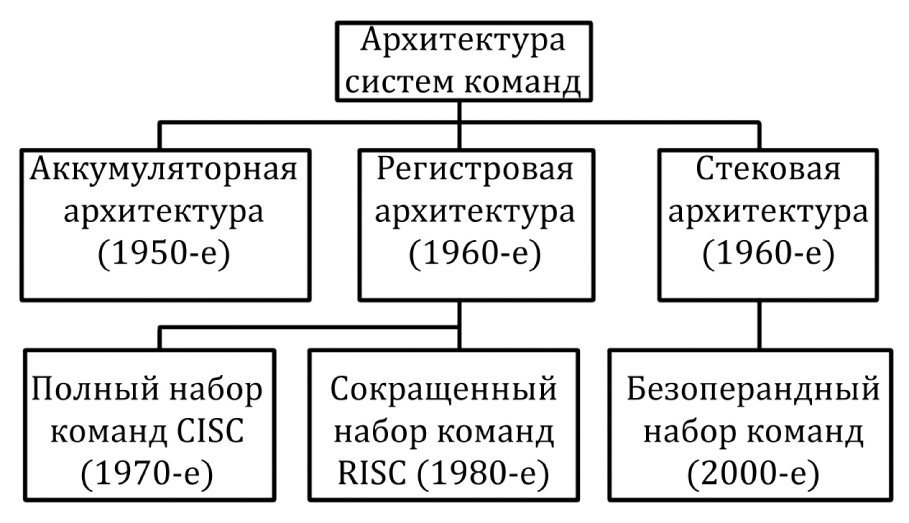
\includegraphics[width=10cm]{9_3}
\caption{������������� ������ ������}
\label{commands}
\end{figure}
\section{�������� ���������� ���}
���������� � ������ �������� ���������� ��� � �����, ���������������� ��� �� ��� ��������:
\begin{itemize}
  \item ������� ������� ��������������� ����������, ����������� ���������, �������� �������� ���������� � ������;
  \item �������� ��������� ��������� ������, ��������� �� ���� ������������� �����;
  \item �������� ������� ����������;
  \item ���������������� ���������������� ����������, ���������� ���������� �������� ������ �� ������ � �� �����������; ;
  \item �������� ���������;
  \item ������ ������� ��������� �����;
  \item ������� ������ �������� � ����������� �������� ����������;
  \item ��� � �������������� ����� � ����� � ��������� ������ � ������������ �������� ��� �������;;
  \item ��������, �������������� ��������� �������� ������ � ��������� ����������.
\end{itemize}
\section{������� ����������}
\begin{figure}[h]
\centering
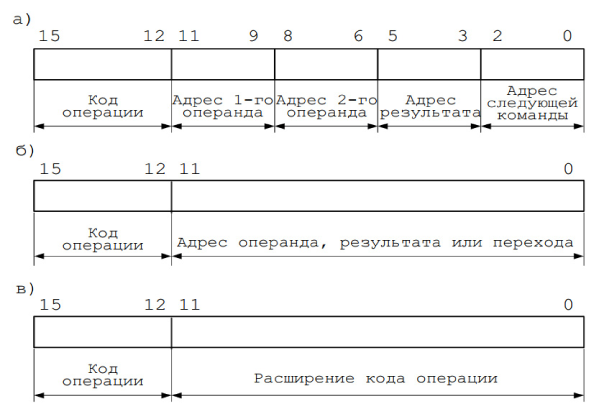
\includegraphics[width=\textwidth]{9_4}
\caption{������� ������ ����������: �) �������������, �) ��������, �) �����������}
\end{figure}
\begin{center}
  \textbf{����� ���������� ������ �����������}
\end{center}
������ ���� ���������� ������� ����� �������� � ���� ��������� �����:
\begin{itemize}
  \item ���������� ������ ������� (���) - ������� ������ ��������� �� ��������� ������, ���������� �������;
  \item ������� ������� (��) - ��������� � ������ ������ �� ������, ���������� � �������� ������, ���������� �������;
  \item ������������� ������� (��) - ��������� ����������, ��� �� ������� (��������, ���������, ������� � ��� �����);
  \item ���������� ������ �������� (���) - ���� ������� ��������, �� ������������ ���������� ������ ��������, ������� �������� �������;
  \item ������� �������� (��) - ��������� � ������ ������ �� ������, ���������� � �������, ���������� ��������;
  \item ���������� �������� �������� (���);
  \item ������ ���������� (��).
\end{itemize}
\begin{center}
  \textbf{����������� ��������� ������}
\end{center}
��� ���������� ����� ������ �������, ���������� ����������� 4-7 ��������. ��� ���������� ������ ��������������� (��� ��� ������ ������ ����������) ��������� ������� ����� �����, ���� ��������� ������������ ������. �������, ��� ����� ��������� ������� �� �������� ���������, ��� ����������� �������� �������� ������.
\begin{figure}[h]
\centering
������ 5-���������� ��������� � �������� RISC-����������:
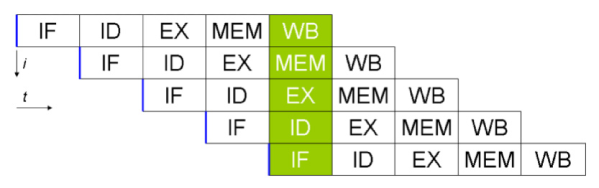
\includegraphics[width=\textwidth]{9_5}
\end{figure}
\begin{description}
  \item[IF] - ���+�� (���������� ������ ������� � ������� �������);
  \item[ID] - ��+���+�� (������������� �������, ���������� ������ ��������, ������� ��������);
  \item[EX] - ��� (���������� �������� ��������);
  \item[MEM] - �� (������ ����������);
  \item[WB] - �� (������ ����������);
\end{description}
�����, ��� ���� ������ ������� ��������� �� ����� WB, ������������ ���� ���� - ������ ����������. ��� �������� ������ ���� - ���������� �������� ��������, ����� �� �����������, � ��������� ������ �������. � ����� �������, ��� ��������� ����������� ���� �� ����� ����, �������� ������������, �������� ����� ������ ������, ��� ����������� ����������� ������������������.

%\chapter{Организация хранения данных в ЭВМ}
%\section{Устройство памяти}
\begin{enumerate}
 \item Память состоит из адресуемых ячеек (размером 1 - 128 бит). Ячейки в основном организованы по 8 бит и свой собственный адрес имеет только каждый восьмой бит.
 \item Ячейки состоят из запоминающих электрических элементов. Это может быть конденсатор, транзистор, попупроводниковый материал и т.п., умеющий хранить два состояния (заряжен или разряжен - конденсатор, находится в проводящем или непроводящем состоянии - транзистор, имеет высокое или низкое удельное сопротивление - попупроводниковый материал). Есть так же элементы, умеющие хранить три состояния, но эти три состояния сложнее считывать.
 \item Электрический элемент может находиться в одном из двух устойчивых состояний (для хранения 1 бита):
 \begin{itemize}
   \item конденсатор заряжен/разряжен;
   \item транзистор в проводящем/непроводящем состоянии;
   \item полупроводниковый материал имеет высокое/низкое сопротивление.
 \end{itemize}
\end{enumerate}
Одно из таких физических состояний создает высокий уровень выходного напряжения элемента памяти, а другое - низкий. В элементах памяти ряда микроЭВМ это электрические напряжения порядка 4В и 0В соответственно, причем первое обычно принимается за двоичную единицу, а второе - за двоичный нуль (возможно и обратное кодирование.)
\begin{figure}[h]
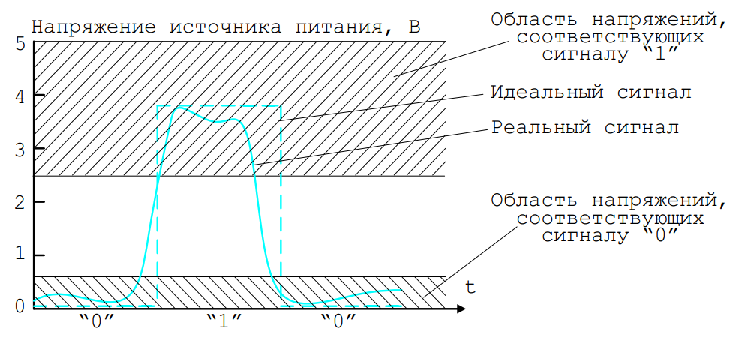
\includegraphics[width=\textwidth]{10_1}
\end{figure}
\\На рисунке показан выходной сигнал элемента памяти (например, одного разряда регистра) при изменении его состояний (при переключениях) под воздействием некоторого входного сигнала. Хотя переход от 0 к 1 и от 1 к 0 происходит не мгновенно, однако в определенные моменты времени этот сигнал достигает значений, которые воспринимаются элементами ЭВМ как 0 или 1. Если сигнал попадает в незаштрихованную область (между 0,5В и 2,5В) то сигнал не распознается.
\\
\\\textbf{Запоминающим элементом} называется элемент, который способен принимать и хранить код двоичной цифры (исходные значения некоторых величин, промежуточные значения обработки и окончательные результаты вычислений). Элементы памяти могут запоминать и сохранять исходные значения некоторых величин, промежуточные значения обработки и окончательные результаты вычислений. Только запоминающие элементы в схемах ЭВМ позволяют проводить обработку информации с учетом ее развития.
\\\textbf{Триггер} - элементарный цифровой автомат, обладающий способностью длительно находиться в одном из двух устойчивых состояний и чередовать их под воздействием внешних сигналов. Состояние $0$ на выходе $Q$ соответствует выключенному состоянию, а $Q = 1$ - включенному. Триггеры осуществляют запоминание информации и остаются в заданном состоянии после прекращения действия переключающих сигналов. Они широко применяются широко применяются при цифровой обработке информации.
\\По способу организации логических связей, определяющие особенности функционирования, различают триггеры:
\begin{itemize}
  \item \textbf{RS-триггер} - меняет свое состояние в зависимости от того, на какой из входов была подана единица. При подаче сигнала на вход $S$ (\emph{Set}) на выходе устанавливается единица. При подаче сигнала на вход $R$ (\emph{Reset}) сигнал на выходе пропадает.
  \item  \textbf{D-триггер} (\emph{Delay} или \emph{Data}) - запоминает (задерживает) состояние входа на один такт. При кратковременной подаче сигнала на $C$ (\emph{Clock}) (обычно, с тактового генератора), запоминает сигнал на входе $D$ (\emph{Data}) и выдает его на выход до следующей итерации.
  \item \textbf{Т-триггер} (\emph{Toggle}) - при подаче сигнала на вход, меняет сигнал на выходе на противоположный.
  \item \textbf{JK-триггер} - аналогичен $RS$-триггеру ($J$ (\emph{Jump}) = $Set$, $K$ (\emph{Kill}) = $Reset$), с одним лишь исключением: при подаче единицы на оба входа, состояние выхода изменяется на противоположное.
\end{itemize}
Из них JK триггер называется универсальным, так как из него можно получить все остальные виды триггеров.
\begin{figure}[!h]
\begin{minipage}{5cm}
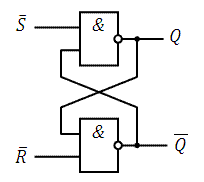
\includegraphics[width=5cm]{10_2}
\caption{Асинхронный RS-триггер на элементах 2И-НЕ (IEC)}
\end{minipage}
\hfill
\begin{minipage}{5cm}
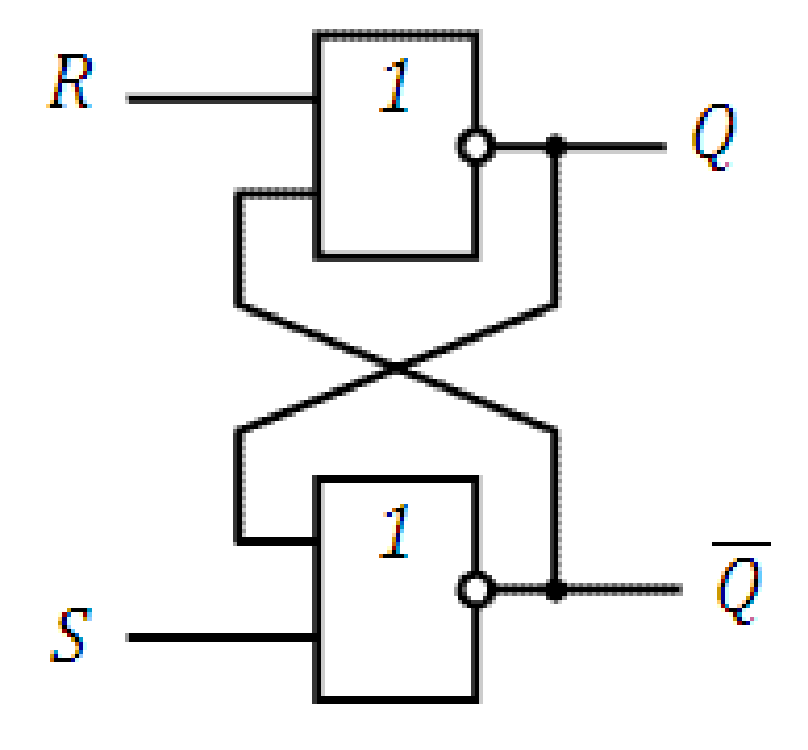
\includegraphics[width=4.7cm]{10_3}
\caption{Асинхронный RS-триггер на элементах 2ИЛИ-НЕ (IEC)}
\label{tag:RS_NOR}
\end{minipage}
\end{figure}

\textbf{Регистры} - это узлы ЭВМ, служащие для хранения информации в виде машинных слов или его частей, а так же для выполнения над словами некоторых логических преобразований.
Регистры способны выполнять следующие операции:
\begin{itemize}
  \item установка регистра в состояние 0 или 1 (на всех выходах);
  \item прием и хранение в регистре n разрядного слова;
  \item сдвиг хранимого в регистре двоичного кода слова вправо или влево на заданное значение разрядов;
  \item преобразование кода хранимого слова в последовательный, и наоборот, при приеме или при выдачи двоичных данных;
  \item поразрядные логические операции.
\end{itemize}
\textbf{Счетчики} - узлы ЭВМ, которые осуществляют счет и хранение кода числа подсчитанных сигналов.Они представляют собой цифровые автоматы Мура, в которых новое состояние счетчика определяется его предыдущим состоянием и состоянием логической переменной на входе.
\\Внутреннее состояние счетчиков характеризуется коэффициентом пересчета К, определяющим число его устойчивых состояний. Основными параметрами являются разрешающая способность (минимальное время между двумя сигналами, которые надежно фиксируются) или максимальное быстродействие и информационная емкость.
\\\textbf{Дешифратор (избирательная схема)} - это узел ЭВМ, в котором каждой комбинации входных сигналов соответствует наличие сигнала на одной вполне определенной шине на выходе (комбинационное устройство). Дешифраторы широко используются для преобразования двоичных кодов в управляющие сигналы для различных устройств ЭВМ.
\\\textbf{Шифратор (кодер)} - это узел ЭВМ, преобразующий унитарный код в некоторый позиционный код. Если выходной код является двоичным позиционным, то шифратор называется двоичным. С помощью шифраторов возможно преобразование цифр десятичных чисел в двоичное представление с использованием любого другого двоично-десятичного кода.
\\\textbf{Преобразователи кодов} - это узлы ЭВМ, предназначенные для кодирования чисел. В число преобразователей кодов входят: двоично-десятичные преобразователи, преобразователи цифровой индикации, преобразователи прямого кода двоичных чисел в обратный или дополнительный код и т. д.
\\\textbf{Мультиплексоры} - это узлы, преобразующие параллельные цифровые коды в последовательные. В этом устройстве выход соединяется с одним из входов в зависимости от значения адресных входов. Мультиплексоры широко используются для синтеза комбинационных устройств, так как это способствует значительному уменьшению числа используемых микросхем.
\\\textbf{Демультиплексоры} - это узлы, преобразующие информацию из последовательной формы в параллельную. Информационный вход D подключается к одному из выходов Qi определяемый адресными сигналами A0 и A1.
\begin{figure}[!h]
\begin{minipage}[c]{6cm}
\center{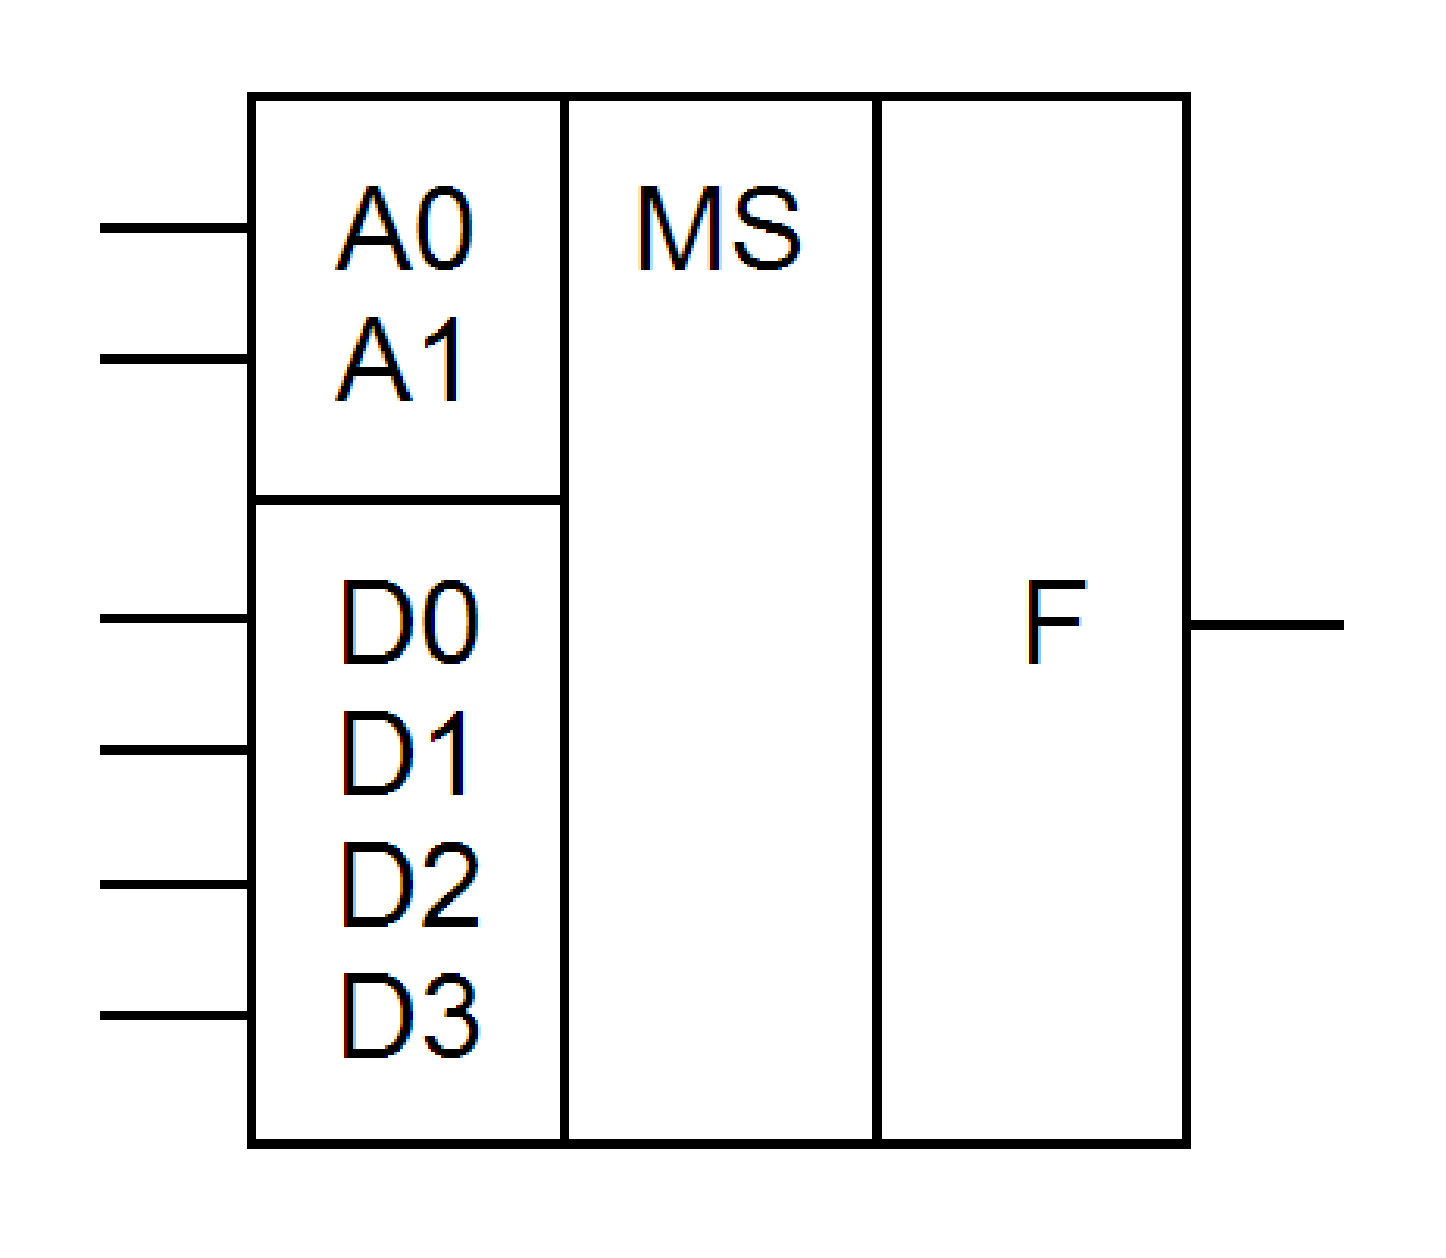
\includegraphics[width=3.5cm]{10_4}}
\caption{Мультиплексор}
\end{minipage}
\hfill
\begin{minipage}[c]{6cm}
\center{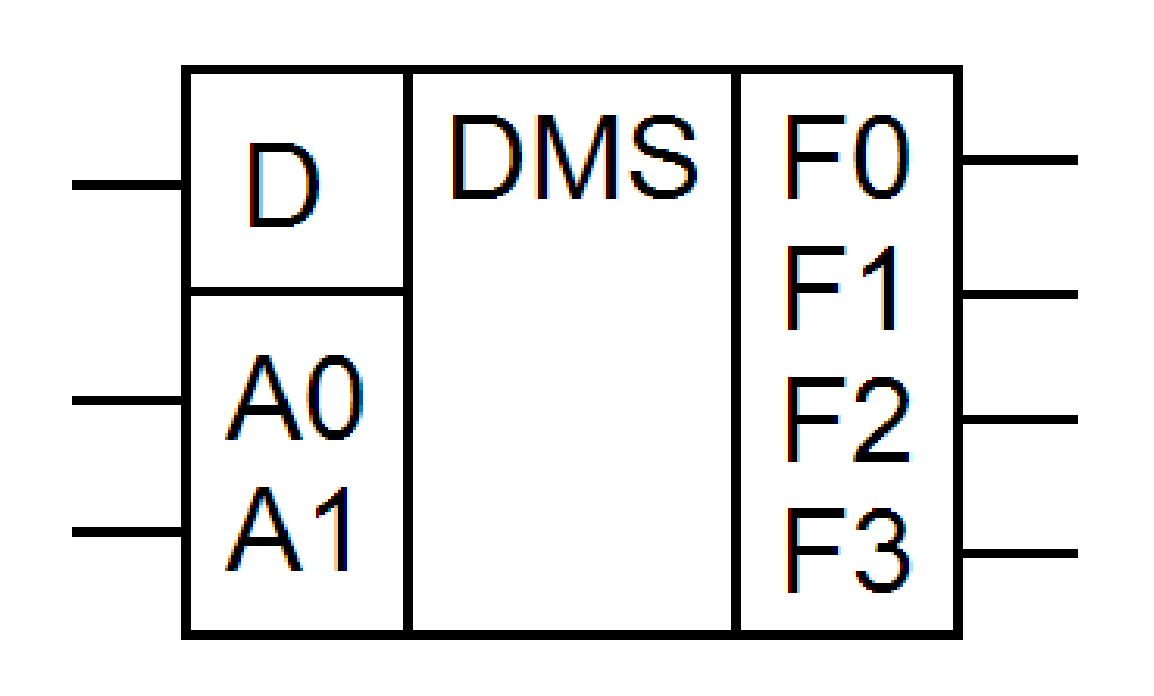
\includegraphics[width=3.5cm]{10_5}}
\caption{Демультиплексор}
\end{minipage}
\end{figure}

\textbf{Сумматор} - это узел, в котором выполняется арифметическая операция суммирования цифровых кодов двух двоичных чисел.
\\Используя одноразрядные сумматоры можно построить многоразрядные сумматоры.
\\\textbf{Шина} - набор коммуникационных линий, каждая из которых способная передавать сигналы, представляющие двоичные цифры 0 и 1. 
\\Электрическая цепь, соединяющая регистр с другим регистром или иным устройством ЭВМ, называется \textbf{шиной (bus)}. \emph{Шина} состоит из параллельных проводов, каждый из которых предназначен для передачи соответствующего бита регистра. Два 8-битовых регистра соединяются между собой шиной из восьми проводов. Про такую шину говорят, что ее ширина равна 8. В действительности шина обычно содержит несколько дополнительных проводов, используемых для передачи сигналов синхронизации и управления, однако подобный анализ структуры шин нас пока не интересует.
\section{Характеристики систем памяти}
\begin{enumerate}
  \item\textbf{ Место расположения:}
  \begin{itemize}
    \item \emph{Процессорная}, то есть на общем кристалле с центральным процессором (ЦП) (регистры, кэш-память 1-го уровня);
    \item \emph{Внутренняя}, то есть на системной плате (основная память (ОП), кэш-память 2-го и последующего уровней);
    \item \emph{Внешняя} (медленные запоминающие устройства (ЗУ) большой ёмкости).
  \end{itemize}
  \item \textbf{Емкость ЗУ} - число бит/байт, которое можно хранить на ЗУ.
  \item \textbf{Единица пересылки.} Для ОП единица пересылки определяется шириной шины данных, то есть количество бит, передаваемых по линиям шины параллельно. Обычно равна длине слова.
  \item \textbf{Метод доступа к данным:}
  \begin{itemize}
    \item \emph{Последовательный доступ} - ЗУ ориентировано на хранение информации в виде последовательности блоков, называемых записями. Для доступа к нужному элементу необходимо прочитать все предшествующие блоки (ЗУ на магнитной ленте);
    \item \emph{Прямой доступ} - каждая запись имеет уникальный адрес, отражающий ее физическое размещение на носителе информации. Обращение определяется как адресный доступ к началу записи плюс последующий последовательный доступ к определённой информации внутри записи (магнитные диски);
    \item \emph{Произвольный доступ} - каждая ячейка памяти имеет уникальный физический адрес. Обращение к любой ячейке занимает одно и то же время и может водиться в произвольной очередности (ОП);
    \item \emph{Ассоциативный доступ} - позволяет выполнять поиск ячеек, содержащих такую информацию, в которой значение отдельных бит совпадает с состоянием одноименных битов в заданном образце. Сравнение осуществляется параллельно для всех ячеек памяти, независимо от ее емкости (кэш-память).
  \end{itemize}
  \item \textbf{Быстродействие} - один из важнейших показателей:
  \begin{itemize}
    \item \emph{Время доступа ($\mbox{Т}_{\mbox{д}}$)} - интервал времени от момента поступления адреса до момента, когда данные заносятся в память или становятся доступными.
    \item \emph{Длительность цикла памяти или период обращения ($\mbox{Т}_{\mbox{ц}}$)} - понятие применяется к памяти с произвольным доступом, для которой оно означает минимальное время между двумя последовательными обращениями к памяти. Период обращения включает в себя время доступа плюс некоторое дополнительное время.
    \item \emph{Скорость передачи} - скорость, с которой данные могут передаваться в память или из нее.
  \end{itemize}
  \item \textbf{Физический тип}
  \begin{itemize}
    \item Полупроводниковая память;
    \item Память с магнитным носителем информации (используемая в магнитных лентах и дисках);
    \item Память с оптическим носителем (оптические диски);
  \end{itemize}
  \item \textbf{Физические особенности} (например, энергозависимость).
  \item \textbf{Стоимость} - стоимость хранения одного бита информации.
\end{enumerate}
\section{Иерархия памяти}
\begin{figure}[!h]
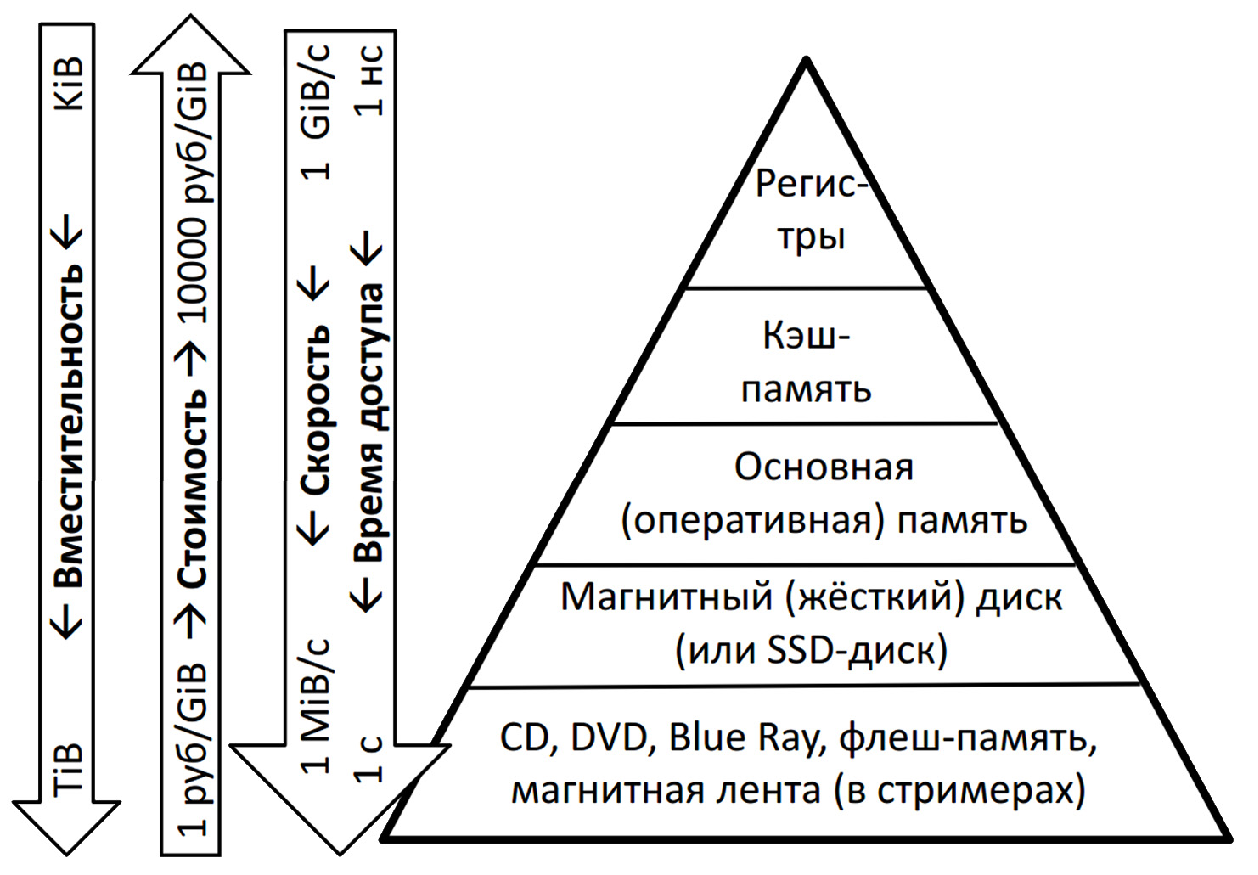
\includegraphics[width=9cm]{10_6}
\end{figure}
Чем меньше время доступа, тем выше стоимость хранения бита. Чем больше емкость, тем ниже стоимость хранения бита, но больше время доступа.

\section{Физическое устройство памяти}
\subsection{Кэш-память}
\begin{wrapfigure}[7]{l}{1.7cm}
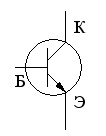
\includegraphics[width=1.7cm]{10_7_(1)}
\end{wrapfigure}
Рассмотрим биполярный \emph{n-p-n} транзистор: К - коллектор, Б - база, Э - эмиттер. На коллектор подано напряжение. Если на базу подать напряжение - транзистор откроется и ток с коллектора пойдет на эмиттер.
\\Небольшая особенность - напряжение на базе должно быть выше, чем на коллекторе (на сколько - зависит от конкретного транзистора, обычно немного. Например, 5В на коллекторе, 6В на базе).
\\
\\Теперь рассмотрим следующую схему:
\\
\begin{minipage}[l]{5cm}
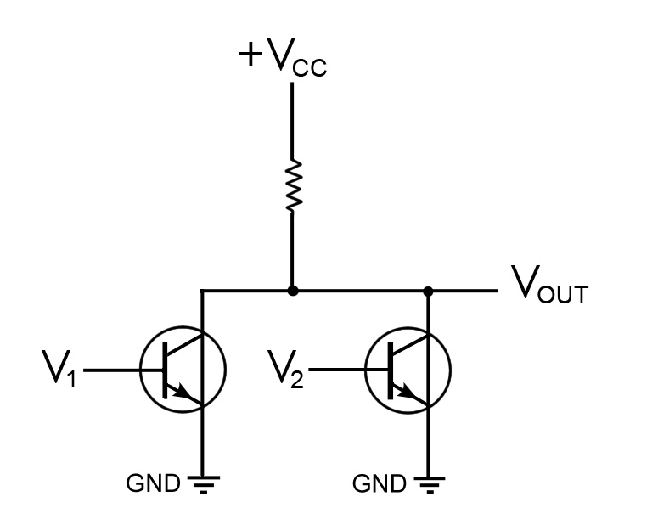
\includegraphics[width=5cm]{10_7}
\end{minipage}
\begin{minipage}[l]{7cm}
$V_{CC}$ - линия питания устройства (например 5В).
\\$GND$ - линия 0В.
\\Если оба транзистора закрыты (на базу не подается напряжение, $V_1$ и $V_2$ равны 0), то ток уходит напрямую с $V_{CC}$ на $V_{OUT}$. В результате получается логическая единица.
\\Если подать напряжение хотя бы на один транзистор ($V_1$ или $V_2$), то ток с $V_{CC}$ будет уходить через транзистор в $GND$ и в $V_{OUT}$ не пойдет. В результате получается логический нуль.
\end{minipage}
\\
\\Так как напряжение на базе должно быть выше, чем на коллекторе (в данном случае, на линии питания $V_{CC}$), а повышенное взять неоткуда, то имеющееся напряжение на $V_{CC}$ занижается с помощью резистора и получается 5В на базе и чуть меньше на коллекторе.
\\
\\Получается, что данная схема реализует логическую функцию ИЛИ-НЕ (ANSI) (также известную как стрелка Пирса) (где $A$ и $B$ соответственно $V_1$ и $V_2$):

\begin{minipage}[l]{4cm}
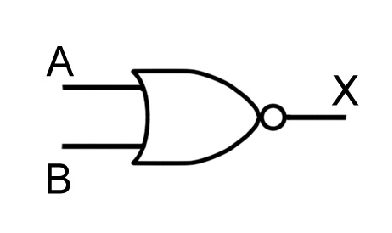
\includegraphics[width=2.8cm]{10_8}
\end{minipage}
\\
\\Таблица истинности для ИЛИ-НЕ:
\begin{table}[!h]
\begin{tabular}{|c|c|c|}
\hline
A & B & X \\
\hline
 0 & 0 & 1 \\
 0 & 1 & 0 \\
 1 & 0 & 0 \\
 1 & 1 & 0 \\
\hline
\end{tabular}
\end{table}
\\Объединим два элемента ИЛИ-НЕ обратной связью.
\begin{wrapfigure}[10]{l}{3.8cm}
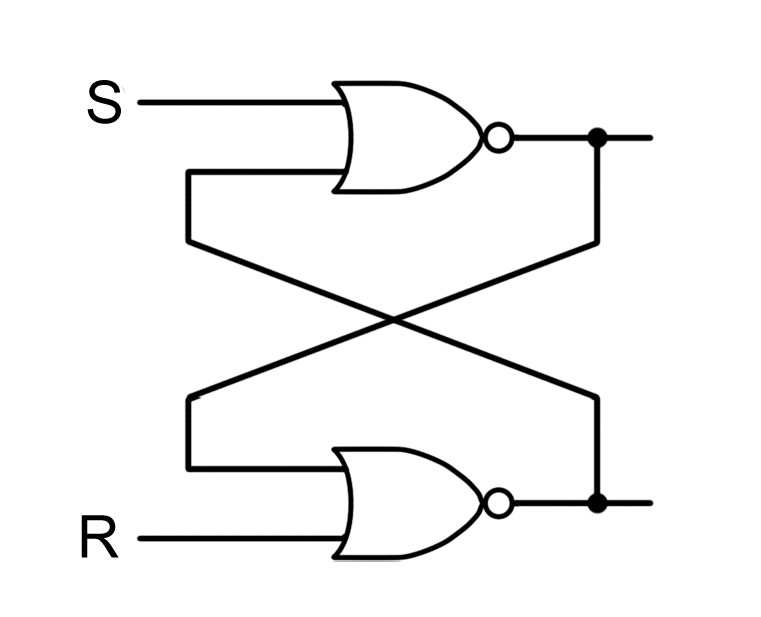
\includegraphics[width=3.8cm]{10_9}
\end{wrapfigure}
Выход одного элемента ИЛИ-НЕ поступает на вход другого. Получилась самая простая память для хранения 1 бита, использующая 4 транзистора.
\\В данном случае, изображен асинхронный RS-триггер (изображен на рисунке \ref{tag:RS_NOR}). Также, память может состоять и из других триггеров.
\\При подаче единицы на вход $S$ выходное состояние становится равным логической единице. А при подаче единицы на вход $R$ выходное состояние становится равным логическому нулю. Если на оба входа $R$ и $S$ одновременно поданы логические единицы, оба выхода переходят в состояние логического нуля, которое является неустойчивым и переходит в одно из устойчивых состояний при снятии управляющего сигнала с одного из входов, иначе говоря, в ячейку может записаться любое значение.
\subsection{Оперативная память}
\begin{wrapfigure}[10]{l}{4cm}
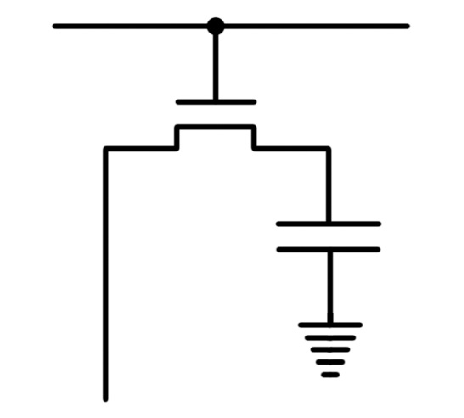
\includegraphics[width=4cm]{10_10}
\end{wrapfigure}
В отличие от кэш-памяти, оперативная память устроена намного проще. Она устроена из 1 конденсатора и 1 транзистора, что дешево и занимает мало места. Один конденсатор легче воспринимать как память (конденсатор разряжен - 0, заряжен - 1). Транзистор нужен с одной целью - чтобы не разряжать постоянно конденсатор. Конденсатор необходимо периодически подзаряжать, а заряжается и разряжается он медленно. Переключить транзистор быстрее чем, зарядить или разрядить конденсатор.
\\Если на базу подано напряжение, транзистор открыт, мы можем считать значение - 1. Если напряжения нет, значение не считывается, записывается 0.
\section{Локальность памяти}
\subsection{Пространственная локальность памяти}
С очень высокой вероятностью адрес очередной команды программы либо следует непосредственно за адресом, по которому была считана текущая команда, либо расположен вблизи него. Такое расположение адресов называется \textbf{пространственной локальностью программы}.
\\Обрабатываемые данные, как правило, структурированы, и такие структуры обычно хранятся в последовательных ячейках памяти. Такая особенность программ называется \textbf{пространственной локальностью данных}.
\subsection{Временн\'ая локальность памяти}
Кроме того, программы содержат множество небольших циклов и подпрограмм. Это означает, что небольшие наборы команд могут многократно
повторяться в течение некоторого интервала времени, то есть имеет место \textbf{временная локальность}.
\\Все три вида локальности объединяет понятие \textbf{локальность по обращению}. Принцип локальности часто облекают в численную форму и представляют в виде так называемого правила "90/10": 90 \%
 времени работы программы связано с доступом к 10\%
  адресного пространства этой программы.
  \subsection{Применение локальности памяти}
 
 Рассмотренные принципы локальности не являются просто любопытным наблюдением. Их использовуют для устранения проблемы узкого места архитектур фон Неймана — шины взаимодействия между процессором и памятью.
 \\
 \\ Память, как правило, работает на меньшей частоте и с меньшей скоростью чем процессор, но программа достаточно часто обращается к памяти. Это приводит к тому, что скорость работы программы и скорость работы компьютера определяется не скоростью работы процессора, а скоростью работы медленной оперативной памяти.
\\Чтобы устранить эту проблему обычно используют кэш, и эффект от него достаточно ощутим: сильный выигрыш в производительности.
Но почему же тогда вместо медленной оперативной памяти не использовать быструю кэш-память? Рассмотрим пример.
\\
\\Так как мы хотим полностью заменить оперативную памать на кэш, то стоимость компьютера увеличится в сто или даже в тысячу раз (оперативной памяти обычно устанавливают гигабайты, а кэш-память измеряется всего лишь мегабайтами). 
\\Чтобы посчитать к какому эффекту это приведёт, будем использовать принцип Парето (\emph{`20\% усилий дают 80\% результата, а остальные 80\% усилий — лишь 20\% результата`}), в соответствии с которым, из-за локальности обращений, 80\% таких обращений попадают в кэш. То есть, при первом обращении большой объем данных приходится копировать из оперативной памяти, что достаточно медленно. Зато далее, в процессе работы программы, с очень высокой вероятностью (в нашем случае – 80\%) при записи/чтении очередной порции данных из памяти мы можем взять её в готовом виде из кэш-памяти. Будем считать, что кэш-память работает в 10 раз быстрее оперативной памяти.
\\Посчитаем, сколько времени понадобится, чтобы выполнить N операций записи или чтения. 
\\Оказывается, что в компьютере, где используется медленная оперативная память, то есть до гипотетической модернизации, время выполнения программы будет равно 2,8N (условно измеряемое в наносекундах).
После замены оперативной памяти на кэш-память, все обращения будут происходить со скоростью кэша, следовательно, общее время сократится до N.
\\
\\
Увидев эти цифры можно сделать любопытный вывод. Мы потратили деньги для того, чтобы ускорить работу памяти в 10 раз, но при этом 10-кратное ускорение памяти привело лишь к трехкратному увеличению производительности. 
В этом и состоит эффект кэширования: вовсе не обязательно устанавливать в компьютере дорогостоящую быструю память, можно обойтись несколькими уровнями кэша, каждый из которых чуть быстрее (а желательно – на порядок быстрее) предыдущего. Это позволит очень эффективно бороться с узким местом принстонской архитектуры.

\section{Порядок хранения байт в памяти}
Существует несколько способов хранения байт в памяти:
\begin{itemize}
  \item \textbf{От старшего к младшему} (англ. \emph{big-endian}): $A_n,\dots,A_0$ запись начинается со старшего и заканчивается младшим. Этот порядок является стандартным для протоколов TCP/IP, он используется в заголовках пакетов данных и во многих протоколах более высокого уровня, разработанных для использования поверх TCP/IP. Поэтому, порядок байтов от старшего к младшему часто называют сетевым порядком байтов.
  \item \textbf{От младшего к старшему} (англ. \emph{little-endian}): $A_0,\dots,A_n$ запись начинается с младшего и заканчивается старшим. Этот порядок записи принят в памяти персональных компьютеров с x86-процессорами, в связи с чем иногда его называют интеловский порядок байт (по названию фирмы-создателя архитектуры x86).
  \item \textbf{Переключаемый порядок} (англ. \emph{bi-endian}). Многие процессоры могут работать и в порядке от младшего к старшему, и в обратном. Обычно порядок байтов выбирается программно во время инициализации операционной системы, но может быть выбран и аппаратно перемычками на материнской плате. В этом случае правильнее говорить о порядке байтов операционной системы.
  \item \textbf{Смешанный порядок} (англ. \emph{middle-endian}) иногда используется при работе с числами, длина которых превышает машинное слово. Число представляется последовательностью машинных слов, которые записываются в формате, естественном для данной архитектуры, но сами слова следуют в обратном порядке.
\end{itemize}
\begin{figure}[h]
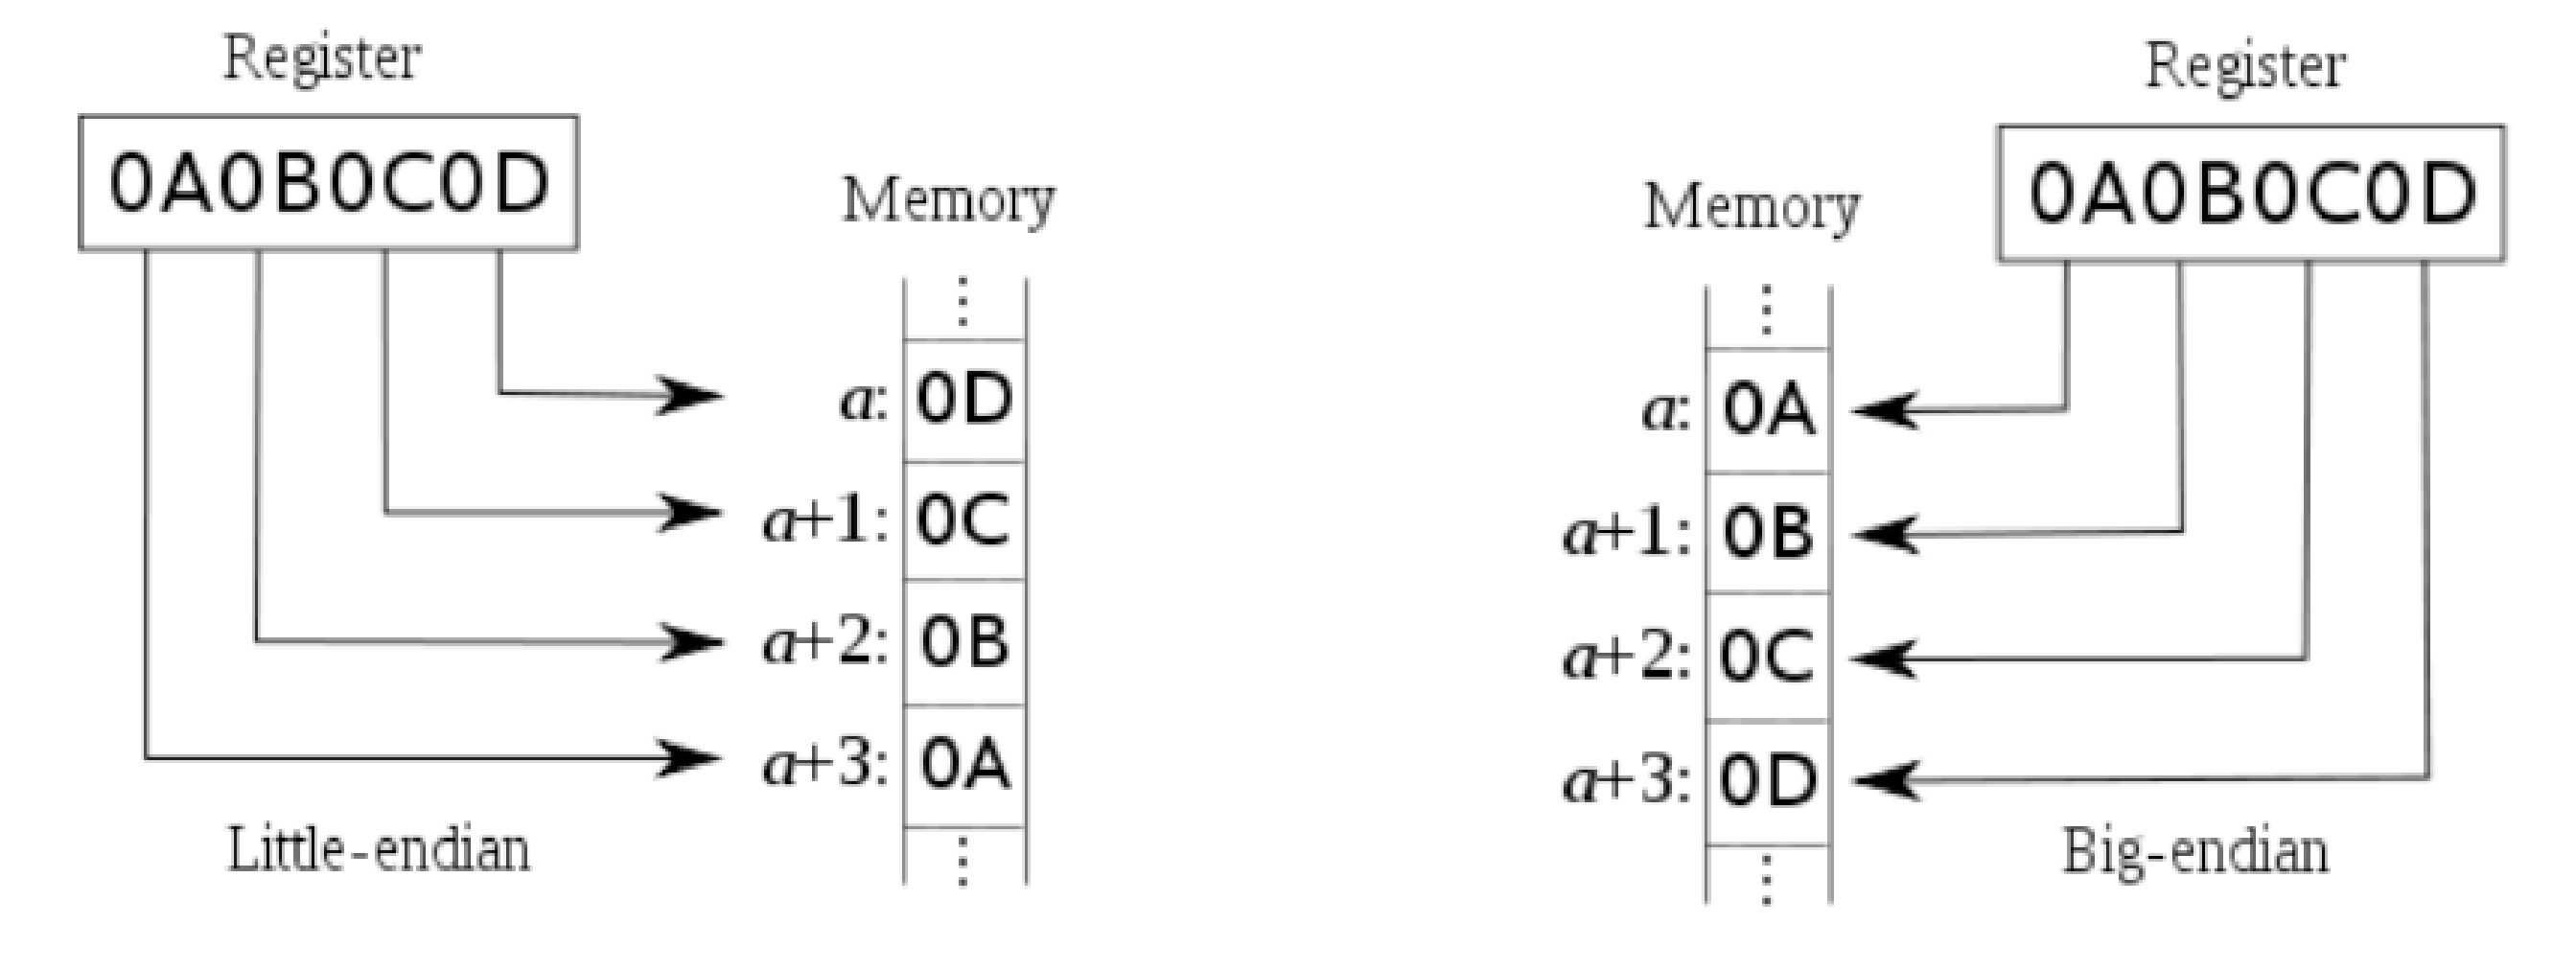
\includegraphics[width=11cm]{10_11}
\caption{Сравнение порядков от младшего к старшему и от старшего к младшему}
\end{figure}

%\chapter{Передача данных в компьютерных сетях}
%\section{Многоуровневая модель OSI (Open Systems Interconnection)}
Процесс передачи данных по компьютерной сети очень сложен, поэтому специалисты International Standards Organization решили разделить его на семь логических независимых уровней. Специалист на одном уровне может работать независимо от специалиста на другом уровне, не мешая друг другу.
\begin{table}[!h]
\begin{tabular}{|c|c|c|}
\hline
№ & Название уровня (layer) & Основная функция \\
\hline
\multirow{2}{*}{7} & \multirow{2}{*}{прикладной (application)} & взаимодействие программы пользователя \\
& & с сетевой подсистемой ОС (API) \\
\hline
\multirow{2}{*}{6} & уровень представления & \multirow{2}{*}{шифрование, сжатие, выбор кодировки}\\
 & (presentation) & \\
\hline
5 & сеансовый (session)  & установление соединения\\
\hline
4 & транспортный (transport)  & надежность доставки, реакция на потери\\
\hline
\multirow{3}{*}{3} & \multirow{3}{*}{сетевой (network)} & маршрутизация, объединение  \\
& & разнородных локальных сетей, \\
& & адресация в глобальной сети (IP) \\
\hline
\multirow{3}{*}{2} & \multirow{3}{*}{канальный (data link)} & связь между узлами одной локальной \\
& & сети, адресация в локальной сети \\
& & (МАС--адрес)\\
\hline
\multirow{2}{*}{1} & \multirow{2}{*}{физический (physical)} & физические характеристики каналов  \\
& & связи и передаваемых сигналов \\
\hline
\end{tabular}
\end{table}
\subsection{Прикладной уровень}
\emph{Субъекты взаимодействия:} пользовательская программа на передающем/принимающем компьютере; ОС.
\\\emph{Объекты взаимодействия:} Пользовательские данные, представленные в "родном" понятном виде для приемной и передающей программы.
\\\emph{Основные функции:} Вызов специальных функций ОС для работы с сетью (API). Программист не обязан знать о внутреннем устройстве
сети, для него передача данных по сети не отличается от сохранения в файл (просто надо вызвать нужную функцию API ОС).
\\\textbf{API} (интерфейс программирования приложений, интерфейс прикладного программирования) (англ. \emph{application programming interface}) — набор готовых классов, процедур, функций, структур и констант, предоставляемых приложением (библиотекой, сервисом) для использования во внешних программных продуктах. Используется программистами при написании всевозможных приложений.
\subsection{Уровень представления}
\emph{Субъекты взаимодействия:} специальное ПО для шифрования, сжатия, кодирования; ОС.
\\\emph{Объекты взаимодействия:} Закодированные пользовательские данные (пользовательская программа уже не может работать с такими данными без декодирования).
\\\emph{Основные функции:} Шифрование, сжатие, выбор кодировки, выбор способа представления порядка байт (little--endian, big--endian).
Каждый этап может выполняться несколько раз разными субъектами.
\subsection{Сеансовый уровень}
\emph{Субъекты взаимодействия:} ОС на компьютере--передатчике; ОС на компьютере--приемнике.
\\\emph{Объекты взаимодействия:} Служебные данные о об установке соединения: логины, пароли, сертификаты, цифровые подписи, пустые пакеты для проверки отсутствия обрывов связи, служебные пакеты с командами типа "запрос соединения", "подтверждение соединения", "разрыв соединения" (т.е. никакие пользовательские данные на этом уровне не передаются).
\\\emph{Основные функции:}
\begin{itemize}
\item Установление соединения (с возможной аутентификацией абонентов).
\item Отслеживание состояния соединения (возможное автопереподключение при обнаружении ошибок).
\item Реагирование на долгую неактивность сеанса связи (например, автоотсоединение по таймауту).
\item Принудительный разрыв соединения при окончании передачи (попутно освобождаются ресурсы ОС, которые хранят информацию о состоянии сеанса).
\end{itemize}
\subsection{Транспортный уровень}
\emph{Субъекты взаимодействия:} ОС; драйвер сетевой карты.
\\\emph{Объекты взаимодействия:} Пользовательские данные, снабженные служебными заголовками для обнаружения проблем передачи (контрольная сумма, порядковые номера фрагментов), служебные пакеты--подтверждения.
\\\emph{Основные функции:}
\begin{itemize}
  \item Отслеживание проблемных пакетов: искаженных, потерянных, пришедших в неверном порядке или дубликатов.
  \item Реакция на обнаружение проблемных пакетов (запрос повторной передачи или игнорирование, сбор целых пакетов из пришедших в разном порядке фрагментов).
  \item Реализация механизма повторной передачи (передается весь файл целиком или только проблемные части).
\end{itemize}
\subsection{Сетевой уровень}
\emph{Субъекты взаимодействия:} ОС; драйвер сетевой карты.
\\\emph{Объекты взаимодействия:} Данные, нарезанные на фрагменты, которые можно передавать в конкретной локальной сети (например, в
проводных сетях Fast Ethernet предельный размер фрагмента $\approx$ 1500 байт, а в сетях Wi--Fi он равен $\approx$ 8000 байт). Каждый фрагмент снабжается глобальным адресом (например, IP--адресом), который понятен в любой локальной сети, но при этом уникален для всей
глобальной сети.
\\\emph{Основные функции:} Маршрутизация в большой сети; обеспечение возможности объединить несколько разнородных локальных сетей в одну сеть.
\subsection{Канальный уровень}
\emph{Субъекты взаимодействия:} драйвер сетевой карты; модуль сетевой карты, который генерирует физические сигналы (ток, радиоволна, пучок света).
\\\emph{Объекты взаимодействия:} Набор битов, полностью готовых к передаче от одного компьютера локальной сети к другому (без выхода в глобальную сеть). Помимо данных пользователя, в этот набор включают адреса приёмника и передатчика внутри локальной сети (например, MAC--адреса).
\\\emph{Основные функции:}
\begin{itemize}
  \item Проверка доступности (свободности) канала связи, если он общий для нескольких абонентов. Например, в Wi--Fi--канал является общим для нескольких устройств в радиусе действия базовой станции, поэтому он не всегда доступен для передачи и каждому устройству приходится ждать своей очереди.
  \item Передача данных и адресация осуществляются только внутри локальной сети (MAC--адрес имеет смысл только в пределах локальной сети, так как он не передаётся в глобальную сеть).
\end{itemize}
\subsection{Физический уровень}
\emph{Субъекты взаимодействия:} модуль сетевой карты, который генерирует физические сигналы (ток, радиоволна, пучок света); проводник сигнала (медный кабель, оптоволокно, радиоэфир).
\\\emph{Объекты взаимодействия:} Физические сигналы (ток, пучок света, радиоволна).
\\\emph{Основные функции:} Выбор носителя сигнала (ток, свет, радиоволна). Выбор свойств проводника сигнала (материал: медь,
оптоволокно; диаметр сечения, сопротивление, предельно допустимая длина). Выбор способа представления цифровых данных в виде физического сигнала (кодирование, модуляция).
\subsubsection{Кодирование}
0 и 1 можно представить в виде разного напряжения электрического тока. Самый интуитивно--понятный способ называется $NRZ$. Однако существует много других способов, устраняющих недостатки $NRZ$ (например, проблему вырождения переменного сигнала в постоянный ток, если передаются много единиц подряд).
\\
\begin{minipage}{\textwidth}
\includegraphics[width=10cm]{11_1}
\begin{center}
Различные системы кодирования данных
\end{center}
\end{minipage}
\\
\subsubsection{Модуляция}
Если сетевая карта умеет генерировать физический сигнал в виде синусоиды, то управляя амплитудой/частотой/фазой этой синусоиды, можно кодировать 0 и 1.
\\
\begin{minipage}{\textwidth}
\includegraphics[width=10cm]{11_2}
\begin{center}
а) информационный сигнал, б) амплитудная модуляция (AM), в) частотная модуляция (FM), г) фазовая модуляция (PM)
\end{center}
\end{minipage}
\subsection{Адекватность OSI--модели}
Не существует ни одной сетевой технологии, в которой бы была идеально реализована вся OSI--модель с четким разделением уровней.
Модель OSI далека от реальности, ее назначение -- быть идеальной абстракцией.
\begin{table}[!h]
\begin{tabular}{r|l}
Реальность & OSI--уровни \\
\hline
Skype & 7,6,5 \\
\hline
FTP & 7,3 \\
\hline
TCP & 7,5,4,3 \\
\hline
IP & 3,4 \\
\hline
Wi--Fi & 1,2 \\
\hline
Fast--Ethernet & 1,2 \\
\end{tabular}
\end{table}
\section{Отличие TCP от UDP}
\begin{table}[h]
\begin{tabular}{|l|c|c|}
\hline
Свойство & TCP & UDP \\
\hline
Установка соединения & $\checkmark$ & $\times$ \\
Разрыв соединения &  $\checkmark$ & $\times$ \\
Подтверждение доставки &  $\checkmark$ & $\times$ \\
Проверка контрольной суммы  & $\checkmark$ & $\checkmark$ \\
Обнаружение искаженных пакетов & $\checkmark$ & $\checkmark$ \\
Обнаружение потерянных пакетов & $\checkmark$ & $\times$ \\
Повторная передача потерянных/искаженных & $\checkmark$ & $\times$ \\
\hline
\end{tabular}
\end{table}
\textbf{TCP} применяют, если необходимо удостовериться, что все данные дошли корректно, получив об этом подтверждение и организовав повторную передачу поврежденных данных (пример: передача почты).
\\\textbf{UDP} применяют либо если канал связи абсолютно надежен, либо если нет смысла повторно передавать потерянные/искаженные пакеты (пример: видео--звонок), но при этом хочется сэкономить на передаче ненужных служебных данных, используемых в ТСР.
\section{Сетевые устройства}

\begin{minipage}{\textwidth}
\includegraphics[width=10cm]{11_3}
\end{minipage}

\begin{center}
  \textbf{Сравнение коммутатора и маршрутизатора}
\end{center}

\begin{table}[!h]
 \begin{tabular}{|c|c|c|}
 \hline
 \multirow{2}{*}{Свойство} & Коммутатор & Маршрутизатор \\
 & (switch) & (router) \\
 \hline
 & & Много (ровно по \\
 Наличие MAC--адреса & Нет & по одному на каждый \\
 & & порт/антенну) \\
 \hline
 & & Много (минимум по \\
 Наличие IP--адреса & Нет & по одному на каждый \\
 & &  порт/антенну) \\
 \hline
 Уровни OSI--модели & 1,2 & 1,2,3 \\
 \hline
 Умение выбирать & Нет (так как в локаль--  & \\
 маршруты & ной сети всегда только  & Да\\
 & один маршрут & \\
 \hline
 & Обмен данными между & Обмен данными  \\
 Назначение & компьютерами внутри & между несколькими  \\
 & локальной сети & локальными сетями \\
 \hline
  \end{tabular}
\end{table}
\textbf{Примечание:} существуют гибридные устройства, совмещающие в себе коммутатор и маршрутизатор (они используются у большинства пользователей домашнего интернета, однако в корпоративных сетях применяются реже).


\end{document} 